%%%%%%%% ICML 2024 EXAMPLE LATEX SUBMISSION FILE %%%%%%%%%%%%%%%%%

\documentclass{article}

% Recommended, but optional, packages for figures and better typesetting:
\usepackage{microtype}
\usepackage{graphicx}
\usepackage{subfigure}
\usepackage{booktabs} % 

 \usepackage{booktabs}
 %\usepackage{rotating}% for sideways figures and tables
\usepackage{longtable}
\usepackage{float}
\usepackage{adjustbox}% for long tables
\usepackage{multicol}
\usepackage{multirow}

% hyperref makes hyperlinks in the resulting PDF.
% If your build breaks (sometimes temporarily if a hyperlink spans a page)
% please comment out the following usepackage line and replace
% \usepackage{icml2024} with \usepackage[nohyperref]{icml2024} above.
\usepackage{amsmath}
\usepackage{hyperref}
\usepackage[capitalize,noabbrev]{cleveref}

% Attempt to make hyperref and algorithmic work together better:
\newcommand{\theHalgorithm}{\arabic{algorithm}}
% https://www.overleaf.com/project/659720fb1ac9f30b08e292f9
% Use the following line for the initial blind version submitted for review:
% \usepackage{icml2024}

% If accepted, instead use the following line for the camera-ready submission:
\usepackage[accepted]{icml2024}

% For theorems and such
\usepackage{amssymb}
\usepackage{mathtools}
\usepackage{amsthm}
\usepackage{multirow} 
\usepackage{multicol}

% if you use cleveref..


%%%%%%%%%%%%%%%%%%
\usepackage{listings}
\usepackage{xcolor}

\definecolor{codegreen}{rgb}{0,0.6,0}
\definecolor{codegray}{rgb}{0.5,0.5,0.5}
\definecolor{codepurple}{rgb}{0.58,0,0.82}
\definecolor{backcolour}{rgb}{0.95,0.95,0.92}

\lstdefinestyle{mystyle}{
    backgroundcolor=\color{backcolour},   
    commentstyle=\color{codegreen},
    keywordstyle=\color{magenta},
    numberstyle=\tiny\color{codegray},
    stringstyle=\color{codepurple},
    basicstyle=\ttfamily\footnotesize,
    breakatwhitespace=false,         
    breaklines=true,                 
    captionpos=b,                    
    keepspaces=true,                 
    numbers=left,                    
    numbersep=5pt,                  
    showspaces=false,                
    showstringspaces=false,
    showtabs=false,                  
    tabsize=2
}

\lstset{style=mystyle}
%%%%%%%%%%%%%%%%%%

%%%%%%%%%%%%%%%%%%%%%%%%%%%%%%%%
% THEOREMS
%%%%%%%%%%%%%%%%%%%%%%%%%%%%%%%%
\theoremstyle{plain}
\newtheorem{theorem}{Theorem}[section]
\newtheorem{proposition}[theorem]{Proposition}
\newtheorem{lemma}[theorem]{Lemma}
\newtheorem{corollary}[theorem]{Corollary}
\theoremstyle{definition}
\newtheorem{definition}[theorem]{Definition}
\newtheorem{assumption}[theorem]{Assumption}
\theoremstyle{remark}
\newtheorem{remark}[theorem]{Remark}

% Todonotes is useful during development; simply uncomment the next line
%    and comment out the line below the next line to turn off comments
%\usepackage[disable,textsize=tiny]{todonotes}
\usepackage[textsize=tiny]{todonotes}


% The \icmltitle you define below is probably too long as a header.
% Therefore, a short form for the running title is supplied here:
\icmltitlerunning{Emergency Department Decision Support}

\begin{document}

\twocolumn[
\icmltitle{Emergency Department Decision Support using Clinical Pseudo-notes}

% It is OKAY to include author information, even for blind
% submissions: the style file will automatically remove it for you
% unless you've provided the [accepted] option to the icml2024
% package.

% List of affiliations: The first argument should be a (short)
% identifier you will use later to specify author affiliations
% Academic affiliations should list Department, University, City, Region, Country
% Industry affiliations should list Company, City, Region, Country

% You can specify symbols, otherwise they are numbered in order.
% Ideally, you should not use this facility. Affiliations will be numbered
% in order of appearance and this is the preferred way.
\icmlsetsymbol{equal}{*}

\begin{icmlauthorlist}
\icmlauthor{Simon A. Lee}{yyy}
\icmlauthor{Sujay Jain}{zzz}
\icmlauthor{Alex Chen}{yyy}
\icmlauthor{Kyoka Ono}{ddd,eee}
\icmlauthor{Akos Rudas}{yyy}
\icmlauthor{Jennifer Fang}{aaa,bbb,ccc}
\icmlauthor{Jeffrey N. Chiang}{yyy,www}
% \icmlauthor{Firstname5 Lastname5}{yyy}
% \icmlauthor{Firstname6 Lastname6}{sch,yyy,comp}
% \icmlauthor{Firstname7 Lastname7}{comp}
% %\icmlauthor{}{sch}
% \icmlauthor{Firstname8 Lastname8}{sch}
% \icmlauthor{Firstname8 Lastname8}{yyy,comp}
%\icmlauthor{}{sch}
%\icmlauthor{}{sch}
\end{icmlauthorlist}

\icmlaffiliation{yyy}{Department of Computational Medicine, University of California, Los Angeles, CA 90095 USA}
\icmlaffiliation{www}{Department of Neurosurgery, University of California, Los Angeles, CA 90095 USA} % need to get from Dr. Fang
\icmlaffiliation{zzz}{Department of Electrical and Computer Engineering, University of California at Los Angeles, Los Angeles, CA 90095 USA}
\icmlaffiliation{aaa}{LA Health Services, Enterprise Clinical Informatics, Los Angeles, CA}
\icmlaffiliation{bbb}{Harbor-UCLA Medical Center, Department of Emergency Medicine, Torrance, CA}
\icmlaffiliation{ccc}{University of California, Los Angeles, Department of Emergency Medicine, Los Angeles, California}
\icmlaffiliation{ddd}{Department of Statistics and Data Science
       University of California, Los Angeles}
\icmlaffiliation{eee}{Department of Natural Sciences
       International Christian University,
       Mitaka, Tokyo, Japan}


\icmlcorrespondingauthor{Simon A. Lee}{simonlee711@g.ucla.edu}
\icmlcorrespondingauthor{Jeffrey N. Chiang}{njchiang@g.ucla.edu}

% You may provide any keywords that you
% find helpful for describing your paper; these are used to populate
% the "keywords" metadata in the PDF but will not be shown in the document
\icmlkeywords{Machine Learning, ICML}

\vskip 0.3in
]

% this must go after the closing bracket ] following \twocolumn[ ...

% This command actually creates the footnote in the first column
% listing the affiliations and the copyright notice.
% The command takes one argument, which is text to display at the start of the footnote.
% The \icmlEqualContribution command is standard text for equal contribution.
% Remove it (just {}) if you do not need this facility.

%\printAffiliationsAndNotice{}  % leave blank if no need to mention equal contribution
\printAffiliationsAndNotice{\icmlEqualContribution} % otherwise use the standard text.

\begin{abstract}
In this work, we introduce the Multiple Embedding Model for EHR (MEME), an approach that serializes multimodal EHR tabular data into text using \iffalse{our}\fi ``pseudo-notes'', mimicking clinical text generation. \iffalse{method}\fi This conversion \iffalse{from tabular to text}\fi not only preserves better representations of categorical data and learns contexts but also enables the effective employment of pretrained foundation models for rich feature representation. To address potential issues with context length, our framework encodes embeddings for each EHR modality separately. We demonstrate the effectiveness of MEME by applying it to several {decision support} tasks within the Emergency Department across multiple hospital systems. Our findings indicate that MEME outperforms {traditional machine learning, EHR-specific foundation models, and general LLMs,} \iffalse{other machine learning} methods\fi { highlighting its potential as a general and extendible EHR representation strategy.} \iffalse{in EHR, underscoring its effectiveness}\fi
\end{abstract}

\section{Introduction}
In recent years, increased access to Electronic Health Records (EHR) has provided healthcare systems with valuable insights into patients' health histories \citep{idowu2023streams}. This wealth of information makes EHR indispensable for inference tasks, especially as the machine learning community increasingly focuses on healthcare applications. Both traditional and cutting-edge machine learning techniques have been harnessed to aid in specific diagnosis and prognosis tasks \citep{shickel_deep_2018}, with a recent keen interest in incorporating state-of-the-art foundation models, such as Large Language Models (LLMs) \citep{zhao_survey_2023}. These advanced models, pre-trained on extensive and diverse textual corpora, offer a broad understanding across numerous domains, \iffalse{significantly}\fi enhancing their adaptability and effectiveness for various complex tasks. Notably, their ability to generate high-fidelity latent representations can be directly employed in many classification tasks, often demonstrating state-of-the-art performance. However, the adoption of these models, built for natural language and text, has been hampered by the fact that the canonical form of generally available EHR data is tabular, and access to textual clinical notes is generally infeasible due to privacy concerns.

We are particularly interested in integrating Electronic Health Records with Large Language Models because traditional machine learning paradigms often struggle with the heterogeneous nature of EHR data. EHRs are disparate data sources, encompassing a wide array of data types, including numerical (e.g., lab test results), categorical (e.g., diagnosis codes, medication types), and free-text data, while spanning multiple biological domains and scales. This diversity enables comprehensive insights into patient health, treatments, and outcomes but also presents numerous challenges. For instance, EHRs frequently include categories with a large number of classes. Traditional methods like one-hot encoding and conventional feature engineering can obscure the inherent meanings within this data, leading to issues such as inefficient data ingestion, a lack of contextual understanding, and sparse data representations. Addressing these challenges is crucial for making full use of the rich, yet complex, information EHR systems contain.

 \begin{figure*}[t]
   \centering 
   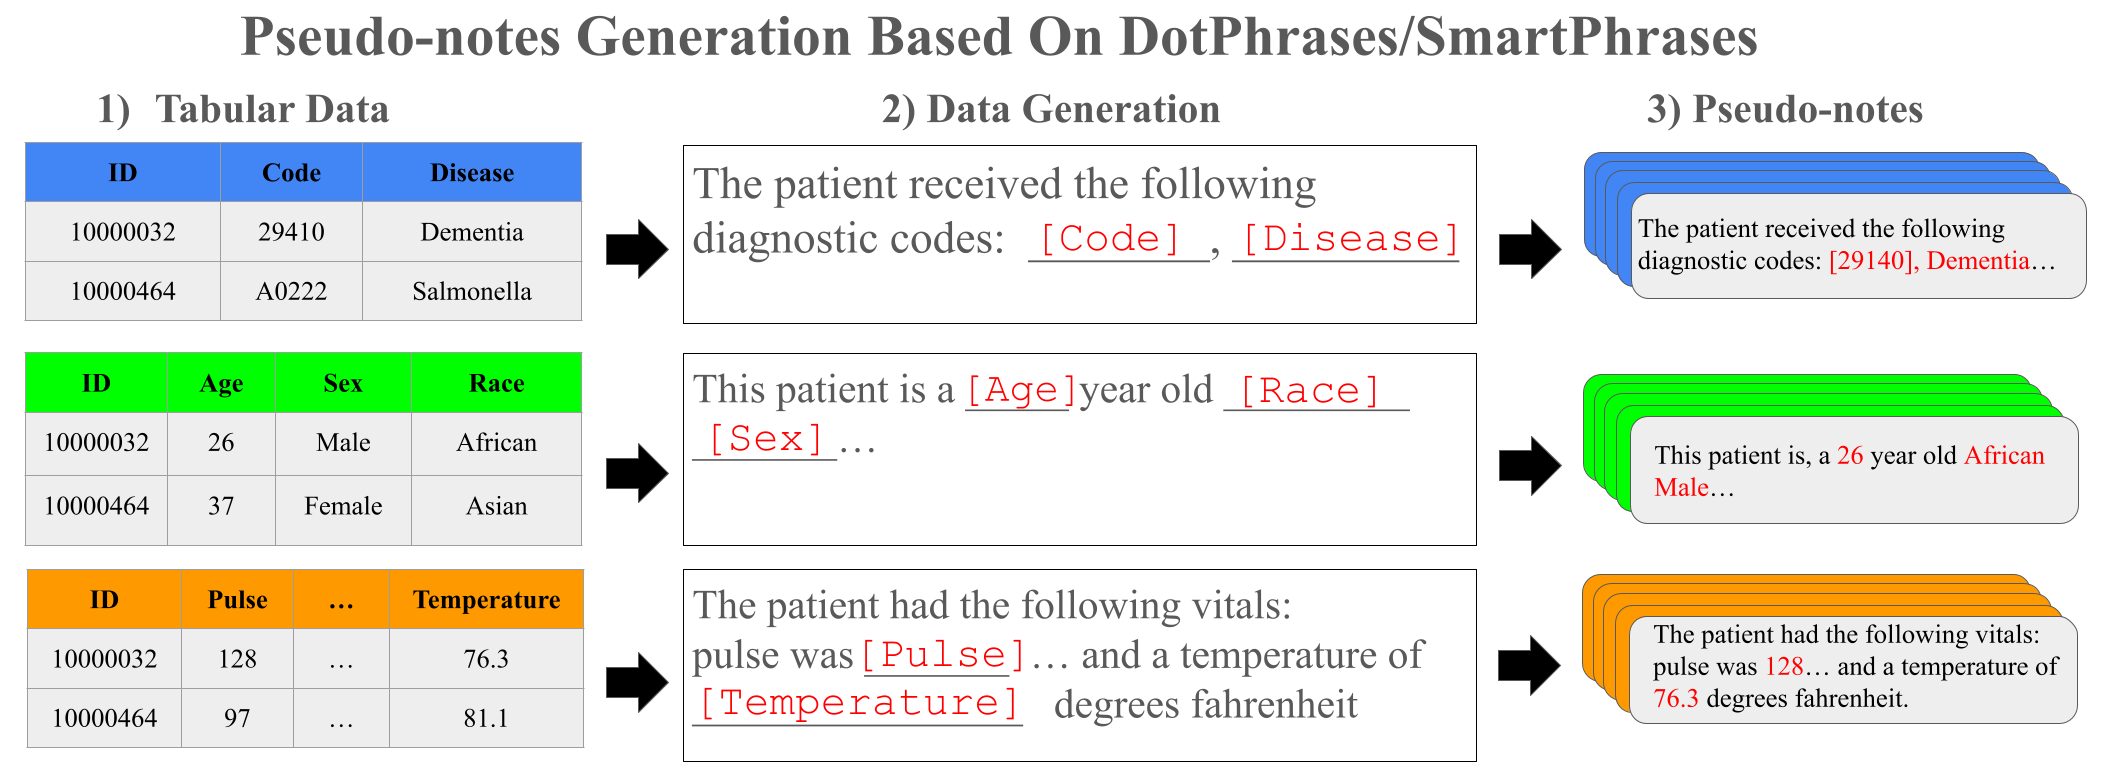
\includegraphics[width=6in]{plots/pseudo.png} 
   \caption{An Overview of Clinical Pseudo-Notes Generation: From Tabular Data to Text Using DotPhrases/SmartPhrases Commonly Employed in Healthcare.}
   \label{fig11} 
 \end{figure*} 

Therefore, in this work, we introduce the \textit{Multiple Embedding Model for EHR (MEME)}, an approach that processes tabular health records and generates textual representations via our ``pseudonotes'' method. Using these clinical pseudo-notes, MEME bridges the gap between tabular EHR data and modern Natural Language Processing (NLP) techniques. We also find that adopting a multiple embedding strategy, where different components of the EHR are encoded separately, yields better results compared to trying to fit all our text into a single heterogenous embedding. We demonstrate this utility by benchmarking MEME against other EHR methods on prediction tasks related to the emergency department. This is an important problem in both machine learning and healthcare because utilizing a patients health history can help predict future events or requirements needed from the emergency department with high precision.

\subsection*{Generalizable Insights about Machine Learning in the Context of Healthcare}
% In this work, we detail the advantages of operating in a textual modality compared to the traditional tabular form. We will also justify our methods and models by providing a comprehensive evaluation of model selection and performance against other models found in the literature. Furthermore, we underscore the significance of this methodology in a clinical context, as it has the potential to streamline decision making within overcrowded hospital settings by predicting outcomes in advance.

In this work, we evaluate text serialization as an interface between tabular electronic health records and large language foundation models. We find our multimodal text serialization approach which separately considers EHR components and leverages the general reasoning capacity of language foundation models outperforms existing  models specifically tailored for healthcare, and that task-specific tuning further outperforms prompting-based approaches. While we demonstrate these capabilities on several benchmark tasks in the context of the Emergency Department, we expect these findings to be applicable to other decision support settings. We also observe limitations in the context of cross-site model generalizability.  

% XX is an important problem in machine learning and healthcare.  (Make
% sure that the clinicians can see the relevance! \emph{Unclear clinical
%   relevance is a major reason that otherwise strong-looking papers are
%   scored low/rejected.})

% Addressing this problem is challenging because XX.  (Make sure that
% you connect to the machine learning here.)  

% Others have tried, but XX remains tough.  (Acknowledge related work.)

% In this work, we...

% As you write, keep in mind that MLHC papers are meant to be read by
% computer scientists and clinicians.  In the later sections, you might
% have to use some medical terminology that a computer scientist may not
% be familiar with, and you might have to use some math that a clinician
% might not be familiar with.  That's okay, as long as you've done your
% best to make sure that the core ideas can be understood by an informed
% reader in either community.

% \subsection*{Generalizable Insights about Machine Learning in the Context of Healthcare}
% % In this work, we detail the advantages of operating in a textual modality compared to the traditional tabular form. We will also justify our methods and models by providing a comprehensive evaluation of model selection and performance against other models found in the literature. Furthermore, we underscore the significance of this methodology in a clinical context, as it has the potential to streamline decision making within overcrowded hospital settings by predicting outcomes in advance.

% In this work, we evaluate text serialization as an interface between tabular electronic health records and large language foundation models. We find our multimodal text serialization approach which separately considers EHR components and leverages the general reasoning capacity of language foundation models outperforms existing  models specifically tailored for healthcare, and that task-specific tuning further outperforms prompting-based approaches. While we demonstrate these capabilities on several benchmark tasks in the context of the Emergency Department, we expect these findings to be applicable to other decision support settings. We also observe limitations in the context of cross-site model generalizability.  

% In this work, we evaluate text serialization as an interface between tabular electronic health records and large language foundation models. We find our multimodal text serialization approach which separately considers EHR components and leverages the general reasoning capacity of language foundation models outperforms foundation models specifically tailored for healthcare, and that task-specific tuning further outperforms prompting-based approaches. While we demonstrate these capabilities on several benchmark tasks in the context of the Emergency Department, we also observe limitations in the context of model generalizability.  

% This section is \emph{required}, must keep the above title, and should
% be the final part of your introduction.  In about one paragraph, or
% 2-4 bullet points, explain what we should \emph{learn} from reading
% this paper that might be relevant to other machine learning in health
% endeavors.

% For example, a work that simply applies a bunch of existing algorithms
% to a new domain may be useful clinically but doesn't increase our
% understanding of the machine learning and healthcare; if that study
% also investigates \emph{why} different approaches have different
% performance, that might get us excited!  A more theoretical machine
% learning work may be in how it enables a new kind of clinical study.
% \emph{Reviewers and readers will look to evaluate (a) the significance
%   of your claimed insights and (b) evidence you provide later in the
%   work of you achieving that contribution}

\section{Related Work}

\subsection{LLM \& Tabular Data}

An ongoing research area involves applying LLMs to tabular data. Several works have focused on using canonical tabular data with existing foundational models, as referenced in \citep{zhang2023towards} and \citep{slack2023tablet}. Additional efforts include utilizing EHR in their canonical form with foundational models, as seen in (\cite{shi2024ehragent}; \cite{wang2023meditab}). A more recent approach involves constructing patient summaries directly from tabular data using LLMs for natural integration into future NLP tasks, highlighted by \citep{ellershaw2024automated} and \citep{hegselmann2024data}. However, such methods have not accounted for the potential for hallucinations by these LLMs, especially in medical applications, as highlighted by \citep{lee2024large}.

Therefore, researchers have explored better methods for converting tabular data into textual formats that harmonize better with LLMs. There are current efforts proposed by \citep{arnrich2024medical} to have some standard for EHR data (Medical Event Data Standard) which comply with existing models. Other previous works \citep{hegselmann2023tabllm}to represent tabular data have led to the development of a novel concept referred to as ``stringified" or serialized tabular data. This technique transforms tabular data into a text-based format, either as a simplified list (e.g., Age: 42, Height: 143cm, ...) or through serialized sentences. Such a transformation allows for a more seamless integration of diverse data types into language models, enabling their analysis with advanced machine learning techniques. The growing interest in this area has facilitated the application of state-of-the-art language models to tabular data, often achieving superior performance compared to traditional machine learning models in scenarios with minimal or no training data. This capability has been demonstrated through a text-to-text prompt-based approach that uses serialized tabular data, leveraging the vast knowledge encapsulated within the parameters of LLMs for various zero-shot and few-shot learning tasks, as illustrated in \citep{hegselmann2023tabllm}. 

Moreover, another study explored the integration of paired datasets (e.g., images) for game data, incorporating both tabular textual and visual fields cohesively for predictive tasks. This was achieved using BERT models to handle the textual component of the datasets \citep{lu2023MuG}, showcasing their versatility in processing complex data structures and blending different types of information seamlessly. Such integrative approaches suggest new possibilities in applying LLMs beyond traditional text-based applications.

\subsection{LLMs, Transformers \& EHR}
Transformer based models and LLMs have also been increasingly applied to EHR data \citep{kalyan_ammu_2022}. These applications tend to fit in one of two paradigms as identified by \citep{wornow_shaky_2023}: One approach that operates upon structured information captured within the EHR and another that operates upon clinical text with recent methods involving multimodal approaches. 

Models developed to represent structured EHR data are generally based on the BERT architecture \citep{kalyan_ammu_2022}. Broadly speaking, these approaches represent the electronic health record as a sequence of events (\cite{wornow2024ehrshot}; \cite{hur2023genhpf}; \cite{hur2022unifying}). For example, BEHRT and its derivatives CEHR-Bert, construct sequences of diagnostic codes and visit metainformation to be compatible with the BERT framework \citep{li_behrt_2020, li_hi-behrt_2021, rasmy_med-bert_2021, pang_cehr-bert_nodate}. They are able to predict future outcomes of visits following a in-context learning/chain-of-thought (CoT) approach, now very popularized in LLM research \citep{wei2022chain}. These models are better adapted to currently available healthcare data due to deidentification and standardization efforts (e.g., OHDSI/OMOP \citep{noauthor_omop_nodate}). 

Notably, nearly all approaches treat EHR data as a single heterogeneous data source, despite the fact that EHR covers data across multiple biological scales and clinical domains (e.g., billing-related diagnostic codes, molecular blood tests, vital-sign measurements). Indeed, more recently, EXBEHRT found that separately representing the components of EHR offers several benefits, including improved performance, shortened sequence length, and fewer required parameters \citep{rupp_exbehrt_2023}.

Another approach directly operates upon clinical notes, which are in the form of natural text. The primary advantage of these approaches is the ability to incorporate pretrained models, such as GPT, BioBert, PubMedBert, etc. \citep{roy-pan-2021-incorporating, chief-bert}. However, these data are challenging to acquire, with nearly all applications restricted to a single database (MIMIC-III, \citep{johnson_mimic-iii_2016}). Recently, efforts have been made to begin multimodal analysis, where groups analyze different data from the EHR (imaging, waveforms, etc.) for predictive tasks. MC-BEC uses all available data within their in-house dataset and performs a multilabel classification on various EHR tasks \citep{chen2023multimodal}. Other attempts have unified imaging data with text \citep{khader2023medical}, and imaging data with structured EHR for various analyses \citep{zhou2023transformer}.

Therefore, in this work, with the continued development of transformer and LLM methods, we develop our own approach that can capture a joint representation of multimodal (e.g. arrival, triage, etc.) structured EHR data. We do so by constructing ``pseudo-notes" out of raw EHR tabular data contained within the MIMIC-IV and our institutional dataset. We then feed this data into a foundation model encoder to obatin representations before finally processing it through a feed forward network with self attention to train a classifier model to predict various binary classification tasks related to the emergency department. 

% Make sure you also put your work in the context of related
% work.  Who else has worked on this problem, and how did they approach
% it?  What makes your direction interesting or distinct?

\section{Benchmarks}
\label{data}

This paper focuses on binary prediction tasks around Emergency Department disposition and decompensation defined in \citep{chen2023multimodal}. \iffalse EHR ED Prediction, utilizing EHR ED data to anticipate class labels for various downstream binary classification tasks. \fi We test our multimodal method's ability to be used in both single classification and multilabel classification tasks benchmarked against other tabular-based and textual-operating machine learning models. This assessment aims to demonstrate the performance advantages of adopting a text-based and multiple embedding strategy.
\subsection{Benchmark tasks}


\begin{enumerate}
        \item \textbf{ED Disposition (Binary Classification):} Our first objective is to predict ED Disposition, determining where patients were sent after their Emergency Room visit, based on EHR measurements recorded during their stay in the ED. We frame this as a binary classification problem, distinguishing whether the patient was discharged home or admitted to the hospital.
        
        \item \textbf{ED Decompensation\iffalse Tasks \fi (Multilabel Binary Classification):} Our subsequent objective is to analyze the subset of patients admitted to the hospital and predict various other measures related to the ED. In this set of tasks, we adopt a multilabel binary classification approach, where the model predicts three separate ED tasks simultaneously. The first task involves predicting the patient's next discharge location, distinguishing between home and other facilities (not home). The second task is predicting the requirement for Intensive Care Unit (ICU) admission.
        And the last task
        is predicting patient mortality, specifically whether the patient dies during their 
        hospital stay.  
\end{enumerate}

\begin{table}[h!]
\caption{Prevalence Statistics for Different Benchmark Tasks in the MIMIC-IV and Institutional Datasets, indicating the proportion of samples in which these outcomes occurred.}
\label{prevalence-table}
\begin{center}
\begin{small}
\begin{sc}
\begin{tabular}{lcc}
\toprule
Task & MIMIC-IV & Institutional \\
\midrule
ED Disposition & 0.395 & 0.253 \\
\bottomrule
Discharge Location & 0.449 & 0.381 \\
ICU & 0.197 & 0.157 \\
Mortality & 0.029 & 0.031 \\
\bottomrule
\end{tabular}
\end{sc}
\end{small}
\end{center}
\end{table}

 In Table \ref{prevalence-table}, we detail the classification objectives and provide a summary of dataset statistics related to the prevalence of each label in these tasks.

\subsection{Data Source}

Our study sources data from the Medical Information Mart for Intensive Care (MIMIC)-IV v2.2 database \citep{johnson_mimic-iv_nodate} 
and further evalution is done on our Institutional EHR database. 
We detail the components of this database to further explore the data inputs for our model. 

% The use of these diverse databases allows for \iffalse a comprehensive \fi examination of EHR data across different settings and patient populations, enhancing the generalizability of our findings.

\begin{figure*}[t]
   \centering 
   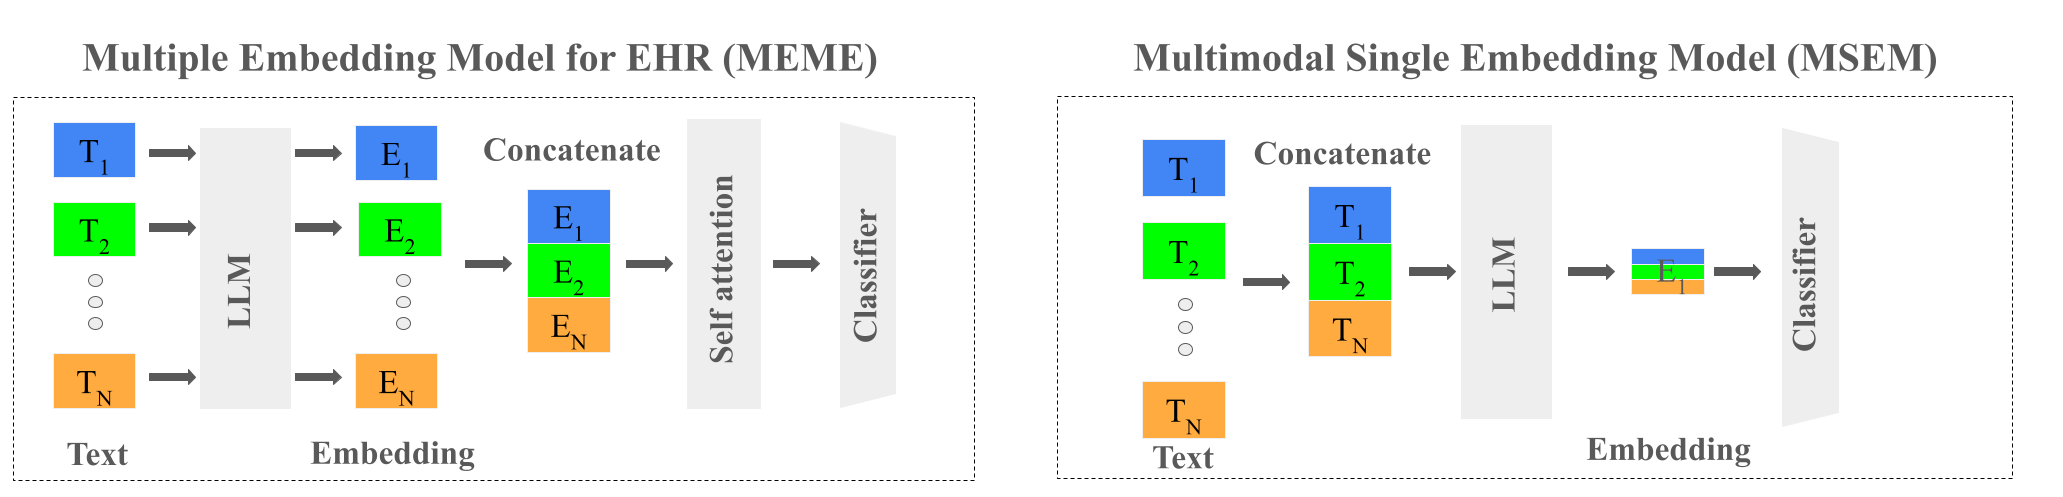
\includegraphics[width=6in]{plots/arc.png} 
   \caption{The Multiple Embedding Model for EHR (MEME) and the Multimodal Single Embedding Model (MSEM) side by side.}
   \label{arc} 

 \end{figure*} 

\begin{itemize}
    \item \textbf{MIMIC-IV ED \citep{Johnson2023MIMICIVED}:} For these downstream tasks, the EHR concepts (modalities) utilized include: \textit{arrival information}, capturing patient demographics and means of arrival; \textit{triage}, documenting patient vitals and complaints at the time of arrival; \textit{medication reconciliation (medrecon)}, detailing prior and current medications taken by the patient; \textit{diagnostic codes} (ICD-9/10 codes) assigned for diagnosis; as well as measurements collected throughout the ED stay, including \textit{patient vitals} and medications received from \textit{pyxis}. All data points across modalities can be combined using a unique Visit or Hospital admission ID (Hadm\_id) and can also be connected to all prediction labels. 
    \item \textbf{Institutional Database:} 
    In our Institutional data, we have access to all data modalities from the MIMIC-IV database with the exception of medication reconciliation (medrecon). However, there may be slight variations in the data across modalities due to the lack of consistency in features in different EHR systems. Our approach is to model our pseudo-notes so that they closely resemble each other. Similar to the MIMIC-IV database, all modalities in our institutional data can be linked using a hospital admission ID and are also associated with all prediction labels.

\end{itemize}

\vspace{-0.2cm}

In the MIMIC-IV database, we analyzed $400,019$ unique visits, each associated with six modalities, contributing to a dataset size of approximately $2.4$ million text paragraphs. For predicting ED Disposition, we use the available data for training, validation, and testing with a set seed for reproducibility purposes. For the three decompensation prediction tasks, \iffalse next three binary multiclass classification tasks, \fi we utilize the subset of visits who were admitted to the hospital from the ED, \iffalse Disposition task, \fi resulting in a sample size of $158,010$ patients. Additionally, in the institutional database, we have a much larger sample size of $947,028$ patients with 5 available modalities (excluding \textit{medrecon}), \iffalse and 1 filler modality (missing medrecon), \fi resulting in approximately $4.75$ million text paragraphs derived from the EHR. We use all available data for the ED disposition task, and the $240,161$ admitted patients were used for decompensation prediction. \iffalse s and reduce the number again for the multilabel classification, resulting in $240,161$ patients. \fi Further breakdowns can be seen in our strobe diagrams attached in the appendix (Section \ref{strober}).

\section{Methods}

\subsection{Clinical Pseudonotes Method}
\label{notes}

We begin by detailing the pseudo-notes method, which was developed in collaboration with a clinical informaticist at our institution. Although various approaches for text generation using Large Language Models (LLMs) have been explored \citep{hegselmann2024data} \citep{ellershaw2024automated}, we identify potential pitfalls in current methodologies due to issues related to hallucinations, as described in \citep{hegselmann2024data} and \citep{lee2024large}. To address these challenges, we employ a more traditional serialization process mimicking SmartPhrases/DotPhrases on the Epic
EHR system \citep{chang2021emr}, which assists in accurately filling in relevant clinical information within a fixed passage to generate the pseudo-notes as shown in Figure \ref{fig11}. We construct separate notes for each clinical modality (e.g., arrival, triage, etc.), resulting in six paragraphs for each patient visit. Additionally, we omit any patient identifiers within the text to mitigate the risk of overfitting on these unique identifiers (e.g., Patient ID, Hospital Admission ID, etc.). While there may be concerns surrounding the similarity between texts, we find that running a BERTopic \citep{grootendorst2022bertopic}, which is analogous to Latent Dirichlet Allocation (LDA), finds unique topics within our corpus of pseudo-notes text. Example Pseudo-notes are attached in the Appendix (\ref{exnotes}).
% We showcase this in Figure 2.

\subsection{Multiple Embedding Model for EHR (MEME) Architecture}
In this section, we outline our model architecture, which is crucial to our end-to-end pipeline. These networks are tailored to process preprocessed and tokenized textual inputs, outputting logits for each class. The class with the highest probability is then selected as the predicted class. We begin by explaining that this approach is designed to embed a patient's modalities separately, accommodating the variable textual lengths associated with different patient visits as described in \citep{rupp_exbehrt_2023}. This strategy addresses a limitation of the BERT architecture, which has a sequence limit of 512 tokens. This method is preferable to the truncation involved in fitting all text into a single heterogeneous embedding, as it better preserves the integrity of the input data and it omits any concerns regarding different ordering strategies. A direct comparison of these approaches can be seen in Figure \ref{arc} which shows our proposed architecture (MEME) over the conventional single heterogenous embedding approach (MSEM).

\subsubsection{Step 1: Generating Embeddings}

In the initial step of our model, we aim to generate embeddings for each EHR concept by feeding tokenized data into our foundational models' encoders, which produce rich, high-dimensional vector representations encapsulating various aspects of a patient's medical history. We choose to freeze the encoder layers, focusing on the training parameters of the subsequent layers dedicated to the prediction task. After generating embeddings for all concepts, we concatenate them into a unified input vector for further processing. This procedure can be mathematically represented as follows: In the model's first phase, modality-specific pseudo-notes are processed and structured into a tokenized format, denoted $D_{\text{tokenized}}$, which outlines a series of unique medical concepts or characteristics ($c_i$) derived from a patient's records. Each concept undergoes transformation via the foundation models' encoder into a high-dimensional vector $\vec{v}_i$, capturing clinical information via context-rich portrayals of each EHR concept. These vectors are then unified into a comprehensive vector $\vec{V}_{\text{concat}}$ through concatenation, laying the groundwork for our multimodal patient embeddings.

\begin{equation}
    \vec{v}_i = \text{FoundationModel}(c_i) \quad \forall c_i \in D_{\text{tokenized}}
\end{equation}
\begin{equation}
    \vec{V}_{\text{concat}} = \text{Concatenate}(\vec{v}_1, \vec{v}_2, \ldots, \vec{v}_n)
\end{equation}

\subsubsection{Step 2: Self-attention Classifier}

In the second step of our network, we introduce a new use case of a self-attention layer \citep{vaswani2017attention} designed to analyze the singular concatenated representation vector, $\vec{V}_{\text{concat}}$, as a unified entity. This approach arises from our intention to interpret aligned modalities collectively, rather than as separate entities, allowing the network to operate comprehensively on the entire vector. It evaluates the relationships between elements within the vector, capturing patterns across different EHR concept vectors. 
% We motivate this method by training a basic self-attention layer from scratch within the feed-forward network, focusing on updating the gradients of this specific component. 
The output from this layer is then directed through a fully connected layer, followed by a ReLU activation function, before being fed into the final classifying layer for prediction. This method, characterized by a unified analysis and attention-based processing, distinguishes our approach from traditional models and is pivotal to the enhanced predictive capabilities of our framework. Mathematically, this process involves transforming the input vector $\vec{V}_{\text{concat}}$ into an attention vector $\vec{V}_{\text{attention}}$ using the self-attention mechanism, further processing it through a fully connected (FC) layer and a Rectified Linear Unit (ReLU) activation to obtain a refined feature vector $\vec{V}_{fc}$, as outlined below:

\begin{equation}
    \vec{V}_{\text{attention}} = \text{SelfAttention}(\vec{V}_{\text{concat}})
\end{equation}
\begin{equation}
    \vec{V}_{fc} = \text{ReLU(FC}(\vec{V}_{\text{attention}}))
\end{equation}
\begin{equation}
    \vec{z} = \text{Classifier}(\vec{V}_{fc})
\end{equation}

The model leverages these refined features, $\vec{V}_{fc}$, in a classifier to produce logits $\vec{z}$, subsequently processed to predict probabilities for ED Disposition or ED Decompensation tasks. The classifier's output is optimized by minimizing Cross Entropy Loss $L$, ensuring alignment of predicted probabilities $\hat{y}$ with true labels $y_i$. For multi-label tasks like ED Decompensation, each logit $\vec{z}_{i,l}$ undergoes individual sigmoid activation $\sigma$, and the model's training involves minimizing a tailored Cross Entropy Loss that aggregates binary cross-entropy losses across all labels for each observation, capturing the multi-label aspects of the data effectively.

% \subsection{Foundation Model Selection}

% We evaluate five different BERT-based models, as well as two other large language models, as potential foundation model backbones for our task, assessing their embedding quality and generalization capabilities. The models under consideration are shown in Table \ref{TableModel} with descriptions for each model. We elected to utilize a BERT-based approach due to its bidirectional embeddings, which provide a more complete view of the context around each word. This allows better reasoning about a word's meaning and role for prediction tasks like the ones presented in this work. In contrast, GPT's left-to-right embeddings may miss important contextual cues from future words, limiting their effectiveness for many prediction tasks that require joint understanding of the full context (\citep{ethayarajh2019contextual}, \citep{schomacker2021language}, \citep{topal2021exploring}).

% The foundation model backbones are evaluated for their effectiveness and generalization capabilities on our specific ED Disposition task, with the goal of selecting the most suitable option for our use case which we will later highlight as the multiple embedding model for EHR (MEME). The results are displayed in Figure \ref{fm}. From this analysis we find Medbert \citep{9980157} which was built on top of \citep{alsentzer2019publicly} to be the most suitable foundation model.

%  \begin{figure}[t]
%    \centering 
%    \includegraphics[width=\columnwidth]{fm_eval.png} 
%     \includegraphics[width=\columnwidth]{generalize.png} 
%    \caption{The benchmark of various foundation models evaluated on ED Disposition. We also explore the model that best generalizes with an additional proprietary instutional dataset for foundation model selection. However as displayed, all models have trouble with Generalization.}
%    \label{fm} 
%  \end{figure} 

\subsection{Preprocessing \& Model Optimization}
\subsubsection{{Missing data imputation and tokenization}} %Preprocessing}

\iffalse{Our data curation process begins by constructing pseudo-notes from our raw EHR data. Initially, we disregard missing entries in the tabular format during the conversion from tabular to text.}\fi {Tabular EHR are converted into pseudo-notes using predefined templates as described above.} {To represent missing data entries, we incorporate} \iffalse{Subsequently, we address the missing data by incorporating} \fi filler sentences such as \texttt{"The patient did not receive any medications"} in cases where the medication reconciliation (medrecon) modality data is missing. We apply this method to all six modalities before feeding them into our tokenizer derived from the MedBERT model. This model utilizes a subword tokenizer optimized to handle out-of-vocabulary (OOV) words by segmenting words into smaller subword tokens or subword pieces, with a vocabulary size of 28,996 subword tokens. We then split our dataset into training, validation, and testing sets using a fixed seed to ensure the replicability of the results found in this study, thus concluding the data preprocessing phase.

 \begin{figure*}[h!]
   \centering 
   \includegraphics[width=5in]{plots/fm_eval.png} 
    \includegraphics[width=5in]{plots/generalize.png} 
   \caption{The benchmark of various foundation models evaluated on ED Disposition. We also explore the model that best generalizes with an additional proprietary institutional dataset for foundation model selection. However, as displayed, all models have trouble with generalization.}
   \label{fm} 
 \end{figure*} 

\subsubsection{Model Optimization}

The models were trained with a batch size of 64, a dropout rate of 0.3, the AdamW optimizer with a learning rate of 5e-5, and a linear learning rate scheduler. For the ED disposition task, we employed Cross-Entropy Loss, and for multilabel decompensation classification, we used Binary Cross-Entropy (BCE) Loss. Training proceeded until a minimum was reached in the validation loss across 10 epochs with early stopping implemented. We tracked F1 scores and loss after each epoch to assess the model's effectiveness. Our computational framework was developed in Python's PyTorch, using large language models available on the HuggingFace \citep{wolf2019huggingface} Platform. For development purposes, we utilized the g4dn.4xlarge EC2 instance from AWS Cloud Services. The model's training and testing were conducted on a single Tesla V100 GPU with 16GB of VRAM to ensure efficient processing.


% Tell us your techniques!  If your paper is develops a novel machine
% learning method or extension, then be sure to give the technical
% details---as you would for a machine learning publication---here and,
% as needed, in appendices.  If your paper is developing new methods
% and/or theory, this section might be several pages.

% If you are combining existing methods, feel free to cite other
% packages and papers and tell us how you put them together; that said,
% the work should stand alone for someone in that general machine
% learning area.  

% \emph{Lack of technical details, such that the soundness of the
%   methods can be verified, is a major reason that otherwise
%   strong-looking papers are scored low/rejected.}

\section{Results}

% overview

\subsection{Model optimization}

% we used ED disposition as teh reference task for selecting the best backbone

\subsubsection{Embedding Model Selection}

We evaluate five different BERT-based models, as well as two other large language models, as potential foundation model backbones for our task, assessing their embedding quality and generalization capabilities. The models under consideration are shown in Appendix Section (\ref{model_des}) in Table \ref{TableModel} with descriptions for each model. We elected to utilize a BERT-based approach due to its bidirectional embeddings, which provide a more complete view of the context around each word. This allows better reasoning about a word's meaning and role for prediction tasks like the ones presented in this work. In contrast, GPT's left-to-right embeddings may miss important contextual cues from future words, limiting their effectiveness for many prediction tasks that require joint understanding of the full context (\cite{ethayarajh2019contextual}; \cite{schomacker2021language}; \cite{topal2021exploring}).

The foundation model backbones are evaluated for their effectiveness and generalization capabilities on our specific ED Disposition reference task, with the goal of selecting the most suitable option for our use case as the multiple embedding model for EHR (MEME). The results are displayed in Figure \ref{fm}. From this analysis we find Medbert \citep{9980157}, which was built on top of \citep{alsentzer2019publicly}, to be the most suitable foundation model.

% \subsection{Ablation Study: Advantages of Multimodal Data \& MEME Approach}
\subsubsection{Multimodal vs unimodal EHR representation}

\begin{figure}[h!]
   \centering 
   \includegraphics[width=3.5in]{plots/results.png} 
   \caption{We performed an ablation study where each modality was used alone to predict the ED Disposition reference task, showcasing the added value of a multimodal data approach.}
   \label{abs} 
 \end{figure} 
\vspace{-0.1cm}
We conduct an ablation study to highlight the benefits of adopting a multimodal data and multiple embedding approach, as illustrated in Figure \ref{abs}. Further results tables can be seen in Appendix Section (\ref{ablation}). This analysis allows us to identify which modalities are most indicative of predicting Emergency Department Disposition based on sets of AUROC and AUPRC results. We observe that no single modality on its own can outperform MEME, as demonstrated through direct comparisons. Additionally, we benchmark MEME against a model designed to encapsulate all multimodal information within a single, heterogeneous embedding. We find that this model's predictive capability is somewhat diminished which is consistent with \citep{rupp_exbehrt_2023} due to truncation and sequence length limitations. This comparison further supports our decision to employ a multiple embedding strategy.

\subsection{MEME vs. reference models}

\begin{table}[H]
\caption{Benchmark study F1. A * denotes that the model operated on tabular data, and a $\dagger$ denotes the model operated on textual (pseudo-notes) data.}
\label{r1}
\begin{adjustbox}{width=\columnwidth}
\begin{small}
\begin{tabular}{l|c|ccc}
\toprule
F1 Benchmark & Dispositon & & Decompensation &\\
Model & ED Disposition & Discharge & ICU & Mortality \\
\midrule
Logistic Regression (Baseline) * &0.799 $\pm$ 0.025&0.549 $\pm$ 0.033& 0.427 $\pm$ 0.036& 0.095 $\pm$ 0.026\\
Random Forest (Baseline) * & 0.826 $\pm$ 0.013 & 0.625 $\pm$ 0.026 & 0.544 $\pm$ 0.048 &  \textbf{0.175 $\pm$ 0.094}  \\
MLP * & 0.841 $\pm$ 0.010 & 0.612 $\pm$ 0.013 & 0.502 $\pm$ 0.019 & 0.097 $\pm$ 0.023 \\
GenHPF \citep{hur2023genhpf} * & --- & --- & ---& --- \\
EHR-Shot\citep{wornow2024ehrshot} *& 0.874 $\pm$ 0.003 & 0.691 $\pm$ 0.008 & 0.560 $\pm$ 0.008 & 0.036 $\pm$ 0.003 \\
MC-BEC\citep{chen2023multimodal} $\dagger$ & 0.912 $\pm$ 0.002& 0.653 $\pm$ 0.006 & 0.545 $\pm$ 0.006 & 0.127 $\pm$ 0.014\\
GPT3.5-turbo $\dagger$ & 0.764 $\pm$ 0.000& --- & --- & ---\\
MSEM $\dagger$& 0.893 $\pm$ 0.003 & 0.622 $\pm$ 0.007 & 0.334 $\pm$ 0.008 & 0.072 $\pm$ 0.014\\
MEME $\dagger$& \textbf{0.943 $\pm$ 0.003} & \textbf{0.698 $\pm$ 0.007} & \textbf{0.572 $\pm$ 0.014} & 0.137 $\pm$ 0.035 \\
\bottomrule
\end{tabular}
\end{small}
\end{adjustbox}
\end{table}
\vspace{-0.6cm}
\begin{table}[H]
\caption{Benchmark study AUROC.}
\label{r2}
\begin{adjustbox}{width=\columnwidth}
\begin{small}
\begin{tabular}{l|c|ccc}
\toprule
AUROC Benchmark & Dispositon & & Decompensation &\\
Model & ED Disposition & Discharge & ICU & Mortality \\
\midrule
Logistic Regression (Baseline) * &0.863 $\pm$ 0.012&0.852 $\pm$ 0.014 & 0.807 $\pm$ 0.017 & 0.768 $\pm$ 0.019\\
Random Forest (Baseline) *& 0.902 $\pm$ 0.010 & \textbf{0.862 $\pm$ 0.014} & \textbf{0.903 $\pm$ 0.016} &   0.847 $\pm$ 0.055\\
MLP *& 0.871 $\pm$ 0.018 & 0.802 $\pm$ 0.011 & 0.767 $\pm$ 0.011 & 0.786 $\pm$ 0.013 \\
GenHPF * & --- & 0.850 $\pm$ 0.000 & ---& \textbf{~0.870 $\pm$ 0.000} \\
EHR-Shot *& 0.790 $\pm$ 0.031 & 0.743 $\pm$ 0.007 & 0.821 $\pm$ 0.18 & 0.827 $\pm$ 0.009\\
MC-BEC $\dagger$& 0.968 $\pm$ 0.002 & 0.708 $\pm$ 0.006 & 0.818 $\pm$ 0.014 & 0.815 $\pm$ 0.006 \\
MSEM$\dagger$& 0.948 $\pm$ 0.002 & 0.552 $\pm$ 0.008 & 0.522 $\pm$ 0.009 & 0.546 $\pm$ 0.023\\
MEME $\dagger$& \textbf{0.991 $\pm$ 0.001} & 0.799 $\pm$ 0.006 & 0.870 $\pm$ 0.015 & \textbf{0.862 $\pm$ 0.006} \\
\bottomrule
\end{tabular}
\end{small}
\end{adjustbox}
\end{table}
\vspace{-0.6cm}
\begin{table}[H]
\caption{Benchmark study AUPRC.}
\label{r3}
\begin{adjustbox}{width=\columnwidth}
\begin{small}
\begin{tabular}{l|c|ccc}
\toprule
AUPRC Benchmark & Dispositon & & Decompensation &\\
Model & ED Disposition & Discharge & ICU & Mortality \\
\midrule
Logistic Regression (Baseline) * &0.874 $\pm$ 0.027&0.628 $\pm$ 0.036& 0.618 $\pm$ 0.034& 0.051 $\pm$ 0.034\\
Random Forest (Baseline) *& 0.902 $\pm$ 0.012 & 0.645 $\pm$ 0.036 & 0.571 $\pm$ 0.047 &  0.102 $\pm$ 0.044  \\
MLP *& 0.866 $\pm$ 0.018 & 0.630 $\pm$ 0.024 & 0.581 $\pm$ 0.026 & 0.077 $\pm$ 0.033 \\
GenHPF * & --- & --- & ---& ---   \\
EHR-Shot *& 0.878 $\pm$ 0.007 & 0.655 $\pm $ 0.012 & 0.655 $\pm$ 0.017 & \textbf{0.246 $\pm$ 0.030} \\
MC-BEC $\dagger$& 0.935 $\pm$ 0.003& 0.657 $\pm$ 0.009 & 0.608 $\pm$ 0.09& 0.174 $\pm$ 0.025 \\
MSEM $\dagger$& 0.890 $\pm$ 0.005 & 0.493 $\pm$ 0.010 & 0.216 $\pm$ 0.009 & 0.037 $\pm$ 0.006\\
MEME $\dagger$& \textbf{0.983 $\pm$ 0.002} & \textbf{0.765 $\pm$ 0.008} & \textbf{0.709 $\pm$ 0.012} & 0.243 $\pm$ 0.034 \\
\bottomrule
\end{tabular}
\end{small}
\end{adjustbox}
\end{table}

In our study, we evaluate the performance of the Multiple Embedding Model for EHR (MEME) against methodologies established by previous research \citep{xie2022benchmarking}, within the domain of Emergency Medicine. This benchmarking study informed comparing various frameworks  previously worked on in the literature as previous state of the art in Emergency Medicine analyses in the case of binary classification. In addition we included several benchmarks from related studies, adopting the methodology of their framework for our tasks.

% \begin{enumerate}
    % \item \textit{Logistic Regression}: Chosen for its simplicity and efficiency in binary classification tasks. Its interpretability and straightforward implementation make it a foundational tool for statistical analysis and machine learning, especially when working with binary or dichotomous outcomes.
    % \item \textit{Random Forest Classifier}: Selected for its interpretability and effectiveness with canonically tabular data, this model facilitates the evaluation of our text-conversion methodology.
    
    % \item \textit{Multi-Layer Perceptron (MLP)}: Chosen for its proficiency in handling high-dimensional tabular data, demonstrating versatility in model application.

    % \item \textit{GenHPF} \citep{hur2023genhpf}: This specialized model leverages the SimCLR framework for self-supervised learning of representations to predict outcomes. \textit{We keep in mind that this method utilizes all the available data from the MIMIC III, MIMIC-IV, and eICU datasets to form predictions.}

    
    % \item \textit{EHR-Shot} \citep{wornow2024ehrshot}: Utilizes the CLMBR-T Base Transformer, as proposed by \citep{steinberg2021language}, to generate patient representations from structured electronic health records (EHR) data, sourced from JSON files. These representations are subsequently employed to pursue our classification objectives, mirroring the strategy used in MEME.
    
    % \item \textit{MC-BEC} \citep{chen2023multimodal}: Adopts the model architecture outlined by Chen et al., which employs embeddings generated from multiple foundational models (\citep{huang2019clinicalbert}, \citep{yan2022radbert}). These embeddings are then used in a Light Gradient Boosting Model (LGBM) for prediction.
    
    % \item \textit{Multimodal Single Embedding Model (MSEM)}: Investigates the value of multimodal representation by concatenating all EHR modalities text and fitting it into a single embedding, as opposed to embedding them separately.

    % maybe add GPT here too, and note that we tested on a random subset (with asterisk in the table) 
% \end{enumerate}

These comparisons were run within and across datasets. The metrics used for evaluation include the F1 scores, the Area Under the Receiver Operating Characteristic Curve (AUROC), and the Area Under Precision-Recall Curve (AUPRC). To ensure robustness, 95\% confidence intervals were generated for each metric by resampling the test set 1,000 times. Our results—comprised of F1 scores, AUROC scores, and AUPRC scores—are presented in Tables (\ref{r1}, \ref{r2},  \ref{r3}).

% \subsection{MEME Outperforms Models}

\subsubsection{MEME vs traditional ML}
We observed that MEME {generally} surpasses the performance of {traditional techniques operating upon tabular EHR {Tables \ref{r1}, \ref{r2}, \ref{r3}}. We evaluated MEME against a logistic regression, random forest, and neural network model proposed on a previous benchmark \citep{xie2022benchmarking}, operating over tabular EHR prior to pseudonote generation.} \iffalse {the tabular Random Forest model and MLP. } \fi Although the Random Forest exhibits a competitive advantage in its AUROC, the imbalanced nature of these tasks makes the benchmarking more nuanced, as it performs inadequately under AUPRC \citep{saito2015precision}.

\subsubsection{MEME vs EHR foundation models}

{EHR-specific foundation models have been recently developed and have shown predictive capabilities across a variety of healthcare applications. We selected the following reference EHR FMs:}

\begin{enumerate}
    \item \textit{GenHPF} \citep{hur2023genhpf}: This specialized model leverages the SimCLR framework for self-supervised learning of representations to predict outcomes. \footnote{\textit{We keep in mind that this method utilizes all the available data from the MIMIC III, MIMIC-IV, and eICU datasets to form predictions while our method only uses that within the MIMIC-IV ED.}}

    
    \item \textit{EHR-Shot} \citep{wornow2024ehrshot}: Utilizes the CLMBR-T Base Transformer, as proposed by \citep{steinberg2021language}, to generate patient representations from structured electronic health records (EHR) data, sourced from JSON files. These representations are subsequently employed to pursue our classification objectives, mirroring the strategy used in MEME.
    
    \item \textit{MC-BEC} \citep{chen2023multimodal}: Adopts the model architecture outlined by Chen et al., which employs embeddings generated from multiple foundational models (\cite{huang2019clinicalbert}; \cite{yan2022radbert}). These embeddings are then used in a Light Gradient Boosting Model (LGBM) for prediction.
\end{enumerate}
We observed that MEME outperformed  MSEM, MC-BEC, EHR-shot models \footnote{The authors have noted that their CLMBR-t transformer does not support non-OMOP vocabulary contained in the MIMIC-IV database, potentially affecting its performance. We highlight this as a limitation in their EHR-shot model.} in this evaluation. We observe that GenHPF outperforms MEME in the AUROC metric, which can be directly compared with our method. However, it is worth mentioning that their approach incorporates all available EHR data from three databases (MIMIC III, IV, \& eICU) to inform these predictions, and thus test set signal may have leaked into the available model weights. Additionally, it is important to note that AUROC alone may not adequately reflect true performance, particularly in the context of our imbalanced classification objectives.


\subsubsection{MEME vs MSEM}
{Consistent with our prior analysis of multimodal EHR representation, we found that MEME significantly outperformed single-modality embedding (MSEM) across all tasks (Tables \ref{r1}, \ref{r2}, \ref{r3}). A primary rationale for the discrepancy between MEME and MSEM could be attributed to MedBERT's, and more generally BERT architectures', token sequence length, which truncates all input after reaching its 512-sequence limit.

\subsubsection{MEME vs LLM prompting}

% \begin{figure}[h!]
%     \centering
%     \includegraphics[width=2in]{icml2024/plots/dispo.png}
%     \caption{Comparison of Classification Accuracies: Training a Classifier (MEME) versus Utilizing a Generative Model (GPT-3.5-Turbo) for Prediction}
%     \label{gpt-meme}
% \end{figure}
%rephrase

\iffalse {In addition to our benchmark, we address the question of whether training a classifier is essential, even with the emergence of generative AI models} \fi  {Given the emergent capabilities of generative AI models (e.g. GPT \citep{radford2018improving}, LLaMA-2 \citep{touvron2023llama}, Claude, etc.), we investigated predictive performance of MEME relative to a zero-shot prompting approach.} \iffalse {To explore this, we conducted a comparison between our} \fi {We compared the} MEME classifier and a zero-shot GPT-3.5-Turbo API using 100 random samples to predict ED disposition. Although our study's sample size is relatively small, we observed a performance gap displayed in Table \ref{r1}, indicating that training a classifier remains preferable for accurate predictions. An additional plot is attached is shown in the appendix Section \ref{gptee}. Even though GPT-3.5-Turbo exhibited performance beyond a random prediction, our findings underscore the continued importance of our approach.

% From Tables \ref{r1}, \ref{r2}, and \ref{r3}, it becomes evident that MEME outperforms all other models, including MSEM, MC-BEC, EHR-shot\footnote{The authors have noted that their CLMBR-t transformer does not support non-OMOP vocabulary contained in the MIMIC-IV database, potentially affecting its performance.}, as well as both baseline models (MLP and random forest classifiers). A primary rationale for the discrepancy between MEME and MSEM could be attributed to MedBERT's token sequence length, which truncates all input after reaching its 512-sequence limit. Additionally, it was observed that MEME surpasses the performance of the tabular Random Forest model and MLP. Although the Random Forest exhibits a competitive advantage in its AUROC, the imbalanced nature of these tasks makes the benchmarking more nuanced, as it performs inadequately when scrutinized through AUPRC. Furthermore, our method currently demonstrates superior performance compared to the standard medical events data models (EHR-shot) in these evaluations. This suggests that converting from a tabular to a textual format with MEME may yield a higher-quality representation of medical concepts, consequently enhancing task prediction performance and improving precision and recall.

% \subsection{Ablation Study: Advantages of Multimodal Data \& MEME Approach}

% \begin{figure}[h!]
%    \centering 
%    \includegraphics[width=\columnwidth]{results.png} 
%    \caption{We performed an ablation study where each modality was used alone to predict the ED Disposition task, showcasing the added value of a multimodal data approach. We additionally included a multimodal method MSEM (Multiple Single Embedding Model) to demonstrate how a single heterogeneous embedding is affected by truncation indicated by its slightly declining performance, further motivating a multiple embedding approach.}
%    \label{abs} 
%  \end{figure} 

% We conduct an ablation study to highlight the benefits of adopting a multimodal data and multiple embedding approach, as illustrated in Figure \ref{abs}. This analysis allows us to identify which modalities are most indicative of predicting Emergency Department Disposition based on sets of AUROC and AUPRC results. We observe that no single modality on its own can outperform MEME, as demonstrated through direct comparisons. Additionally, we benchmark MEME against a model designed to encapsulate all multimodal information within a single, heterogeneous embedding. We find that this model's predictive capability is somewhat diminished due to truncation and sequence length limitations. This comparison further supports our decision to employ a multiple embedding strategy.

% \subsection{Is any of this necessary in the emergence of Generative AI?}

% \begin{figure}[h!]
%     \centering
%     \includegraphics[width=2in]{dispo.png}
%     \caption{Comparison of Classification Accuracies: Training a Classifier (MEME) versus Utilizing a Generative Model (GPT-3.5-Turbo) for Prediction}
%     \label{gpt-meme}
% \end{figure}

% In addition to our benchmark, we address the question of whether training a classifier is essential, even with the emergence of generative AI models (e.g. GPT, LLaMA-2, Claude, etc.). To explore this, we conducted a comparison between our MEME classifier and a zero-shot GPT-3.5-Turbo API using 100 random samples to predict ED disposition. Although our study's sample size is relatively small, we observed a performance gap displayed in Figure \ref{gpt-meme}, indicating that training a classifier remains preferable for accurate predictions. Even though GPT-3.5-Turbo exhibited performance beyond a random prediction, our findings underscore the continued importance of our approach.

\subsection{Generalizability of our Method}

A recent critique of healthcare AI applications identified the lack of external validation and therefore potential overfitting to existing publicly available data. Indeed, we observed that while our approach and our reference models displayed strong within-dataset performance using a train-test split, performance was reduced when externally validated across institution (Figure \ref{bar13}).
These results are analogous to the study of \citep{jiang2023health}, who identified that fine-tuning on local hospital systems can improve general performance due to differences caused by demographics, locality, healthcare accessibility and more. 

\begin{figure}[h!]
\begin{center}
\label{bar}
\centerline{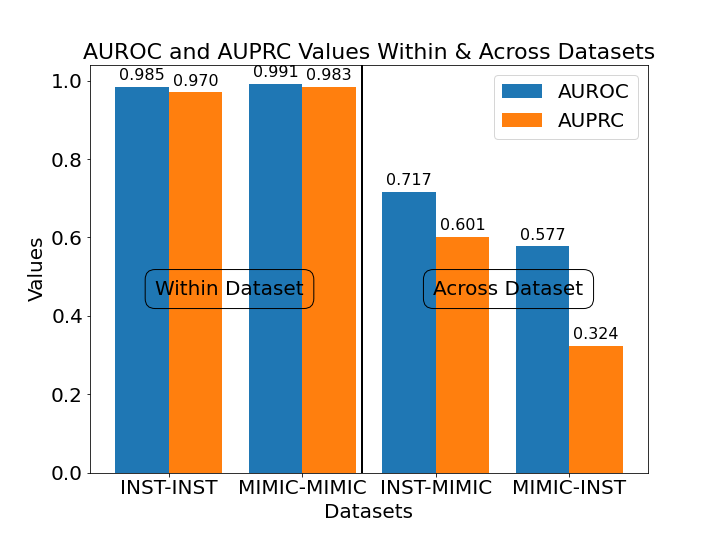
\includegraphics[width=2.5in]{plots/bar2.png}}
\caption{Comparative Analysis of AUROC and AUPRC Values for Intra- and Inter-Dataset Evaluations: This bar chart illustrates the AUROC and AUPRC values of different models, where the models themselves are represented by their training and testing datasets (e.g., MIMIC-MIMIC). \textit{INST stands for institutional dataset}.}
\label{bar13}
\end{center}
\end{figure}
We performed a qualitative error analysis on the top 10 and bottom 10 scoring exemplars in our Institutional dataset to gain insight into this performance gap. Concordant cases were defined as those which the model scored highly and were correctly identified, or scored lowly and correctly not flagged, and Discordant cases were defined as vice versa. No systematic patterns or patient attributes were immediately apparent from investigating the decision making of this model in these groups, necessitating future study. \iffalse{We found no systematic patterns or attributes of patients that explained this gap.}\fi

However, we observed a distribution shift between datasets in terms of EHR features. {We compared the unique tabular values across the two EHR databases and observed only moderate overlap between values and concepts} \iffalse{We additionally explored the heterogeneity of the data inputs within our pseudonotes method, where we identified differences of unique values (i.e. Categorical - Venn Diagram, Numerical - Boxplots) from all the features across our two tabular EHR databases. We find that these results seen in Figure } \fi (Figure \ref{venn}). For a more detailed perspective see appendices (Section \ref{gener3}). This might reflect systematic differences in patient populations or hospital protocols. \iffalse{, appear to be behind this failed generalizability}\fi 

\begin{figure}[h!]
\vskip 0.2in
\begin{center}
\label{bar}
\centerline{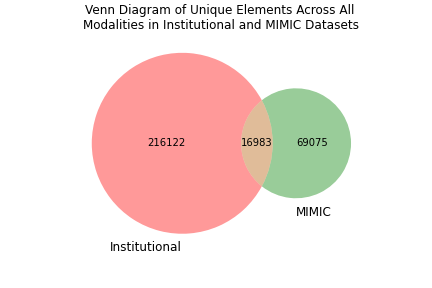
\includegraphics[width=2.5in]{plots/venn.png}}
\caption{Venn Diagram of Unique Features across all modalities respective of both EHR Systems. Note the large differences in features indicating a distribution shift.}
\label{venn}
\end{center}
\vskip -0.2in
\end{figure}

% \emph{This section is optional, and more theoretical work may not need
%   this section.  However, if you are using health data, then you need
%   to describe it carefully so that the clinicians can validate the
%   soundness of your choices.} 

% Describe the cohort.  Give us the details of any inclusion/exclusion
% criteria, what data were extracted, how features were processed,
% etc.  Recommended headings include:

% \subsection{Cohort Selection} 
% This includes choice of criteria and basic numbers, as well as any relevant
% information about the study design (such how cases and controls were
% identified, if appropriate), 

% \subsection{Data Extraction} 
% This includes what raw information you extracted or collected, including any
% assumptions and imputation that may have been used, and 

% \subsection{Feature Choices} 
% This includes how you might have converted the raw data into features that were
% used in your algorithm. 

% Cohort descriptions are just as important as methods details and code
% to replicate a study.  For more clinical application papers, each of
% the sections above might be several paragraphs because we really want
% to understand the setting.

% For the submission, please do \emph{not} include the name of the
% institutions for any private data sources.  However, in the
% camera-ready, you may include identifying information about the
% institution as well as should include any relevant IRB approval
% statements.

% \subsection{Results on Synthetic Experiments}

% \emph{Depending on the claim you make in the paper, this section may
%   not be relevant.}

% Especially if you are developing a new method, you will want to
% demonstrate its properties on synthetic or semi-synthetic experiments.
% Include experiments that will help us understand the contribution of
% the work to machine learning and healthcare. 

% \section{Results on Real Data} 
\section{Discussion \& Conclusion}

In this paper we introduce \iffalse{our model MEME ,}\fi {a Multimodal Embedding Model for EHR (MEME), a representation framework for EHR. MEME is built upon two core concepts: 1) The text serialization of tabular EHR into pseudo-notes, which provides an interface with language foundation models; and 2) the multimodal framing of EHR to reflect the heterogeneity of the underlying data.} \iffalse{an approach for transforming multimodal tabular EHR data into clinical pseudo-notes. This transformation \iffalse{significantly}\fi enhances the interpretability of our data inputs and utility of EHR data in various healthcare-related tasks. The pseudo-notes method not only simplifies data handling but also effectively bridges the gap between traditional EHR formats and advanced NLP techniques employed in modern machine learning.} \fi
{We demonstrate that this combination outperforms traditional ML techniques, EHR-specific foundation models, and prompting-based approaches across decision support tasks in the Emergency Department.} \iffalse{A key finding from our study is the superior performance of the multimodal strategy employed by MEME. It  outperforms a traditional machine learning method, and other methods found in the literature, demonstrating the benefits of encoding different components of EHR separately. This approach allows for a more comprehensive representation of a patient's medical profile, capturing a broader spectrum of medical information crucial for accurate predictions. }\fi

{In addition to the performance advantages demonstrated by our experiments, MEME has several qualitative benefits in terms of portability and extendibility. EHR-specific models, such as BEHRT \citep{li_behrt_2020}, CHIRoN \citep{hill2023chiron}, EHR-shot \citep{wornow2024ehrshot}, etc., rely on data standards and transparent harmonization procedures to ensure interoperability, and their general applicability is severely hampered by the fact that these standards are still being developed and evaluated (e.g., MEDS\_ETL vs OMOP). It is also unclear how these models should be extended to accommodate new and updated medical concepts \citep{arnrich2024medical}. By contrast, the natural language approach is extendible to any data that can be text-serialized, which is more easily adopted by institutions, and can more gracefully handle changes in coding standards, all the while leveraging general reasoning capabilities and increasing medical domain knowledge captured by LLMs. While all of our findings were demonstrated within the Emergency Department setting, we hypothesize that they should generalize into other common decision support scenarios.}

% We expect that this approach is robust and extendible
%qualitative advantages of pseudo-notes in terms of portability:
% 1. smoother data processing; 2. extendible to clinical notes and other data types. 3. extendible to other tasks beyond ED)

% \subsection{Pseudo-notes is smoother for data processing}
% In terms of data handling and preparation, we found that our pseudo-notes method, from raw input to output, was more efficient and easier to handle compared to the benchmarked methods. These methods rely on the Medical Events Data Standard (MEDS\_ETL \citep{arnrich2024medical}), which is still under development. While the comparison of our approach isn't direct, since we are comparing a text based method to a tabular one, we still find this to be worth noting. We identified various issues and dataset limitations with meds\_etl at its current state primarily due to the hardcoding of file transformations within their pipeline. This hardcoding restricts their utility for proprietary (Institution) datasets and non hard-coded datasets (MIMIC-IV ED), where such specific information may not be available. Additionally, their CLMBR-T transformer does not support non-OMOP vocabularies, making it challenging to perform a direct comparison and benchmark of methods. 


% \subsection{JSON Generated Versus Pseudo-notes Method Comparisons}

% We conducted an analysis on the data generation process, comparing text generation via large language models (LLMs) to our pseudo-notes method. We found that inputting JSON data into LLMs like GPT-4 and LLaMA-2, which are not optimized for parsing structured tables, leads to a small degree of ``hallucination." This issue is particularly pronounced in long contexts, critically impacting the integrity of our original data. These findings are underscored in \citep{hegselmann2024data}. However, it's important to note the extensive efforts recently undertaken by groups such as LLaMA Index and detailed in recent studies (\citep{song2023restgpt}, \citep{jiang2023large}, \citep{chen2024beyond}, \citep{yao2023sai}) to mitigate this issue. Nonetheless, given the importance of accuracy and sensitivity in applications like healthcare, we argue that a fill-in approach may offer a more conservative and reliable alternative.




% However, our findings also highlight a significant challenge in the field of EHR analysis: the limited generalizability of models across different hospital institutions. Despite its strengths, the representation derived from the MIMIC-IV Database proved insufficient for generalization across diverse healthcare systems. This underscores the need for more representative publicly available datasets that can generalize to other EHR systems.

% \emph{Depending on the claim you make in the paper, different
%   components may be important for this section.}

% \subsection{Evaluation Approach/Study Design} 
% Before jumping into the results: what exactly are you evaluating?
% Tell us (or remind us) about your study design and evaluation
% criteria.

% \subsection{Results on Application A} 

% Present your numbers and be sure to compare proposed methods against appropriate baselines. 
% You should provide a summary of
% the results in the text, 
% as well as in tables (such as
% Table~\ref{tab:example}) and figures (such as
% Figure~\ref{fig:example}).  
% You may use subfigures/wrapfigures 
% so that figures don't have to span the whole page or multiple figures are side by side.

% \begin{table}[t]
%   \centering 
%   \caption{Description with the main take-away point. Note that the caption should appear \emph{above} the table.}
%   \begin{tabular}{llll}
%   \toprule
%     \textbf{Method} & \textbf{Metric1} & \textbf{Metric2} & \textbf{Metric3} \\
%     \midrule
%     Baseline & 1.1 & 2.3 & 0.1 \\ 
%     NetNet & 41.3 & 31.9 & 77.4 \\ 
%     \bottomrule
%   \end{tabular}
%   \label{tab:example} 
% \end{table}

%  \begin{figure}[t]
%    \centering 
%    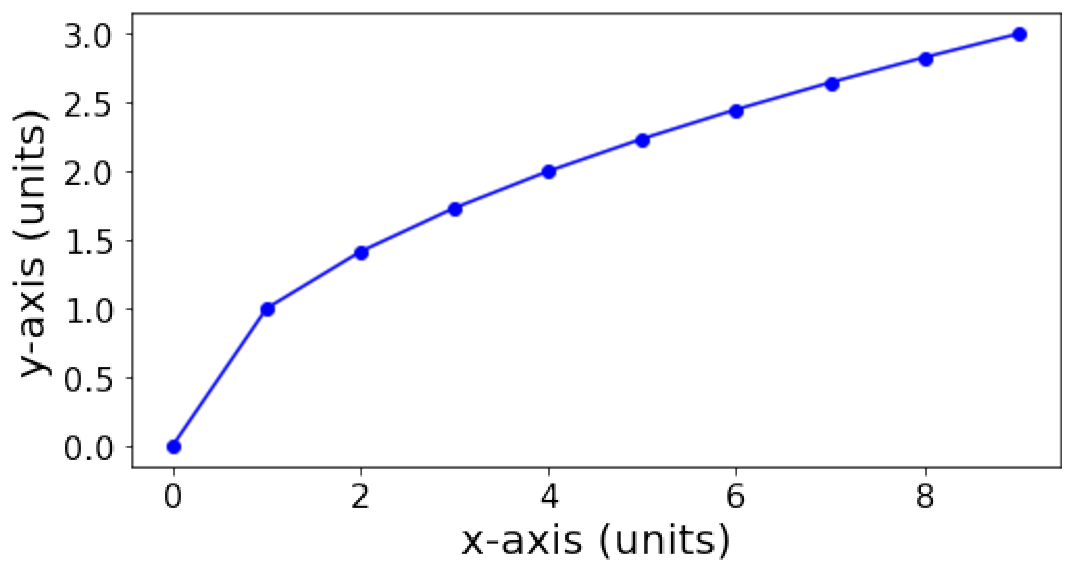
\includegraphics[width=2.5in]{plot.pdf} 
%    \caption{Description with the main take-away point. Note that figure captions should appear below the figure.}
%    \label{fig:example} 
%  \end{figure} 

% \subsection{Results on Application/Follow-up Study B} 

% \section{Required: Discussion} 

% \emph{This is probably the most important section of your paper!  This
%   is where you tell us how your work advances our understanding of
%   machine learning and healthcare.}  Discuss both technical and
% clinical implications, as appropriate\cite{xyz19}.
\paragraph{Limitations}

One crucial limitation of the model is the poorly performing external validity caused by the heterogenous nature of two EHR datasets. 
% While building a training dataset that combines MIMIC and our UCLA EHR, or performing external-site-specific fine tuning could alleviate this performance drop-off, it is important to highlight that different hospital systems may result in generalizability for this model and competitors, as identified by Wornow and colleagues \citep{wornow_shaky_2023}. 
We saw in our results that it is likely that protocols around patient care vary across site and over time such that the same patient would experience different outcomes depending on when and where they experienced care. Therefore we conclude that current models developed on the publicly available MIMIC-IV ED dataset appear to be insufficient for ensuring true generalization across diverse healthcare systems.

Another limitation of this work is our inability to release our private institutional data, due to privacy restrictions and university policy. This highlights the significance of independent benchmarks, and underscores the necessity of external validation, including benchmark datasets and tasks such as MC-BEC \citep{chen2023multimodal}.
\paragraph{Future Works}
\iffalse Some future work that our group is currently exploring includes various use cases for pseudo-notes, as this clinical text can be applied beyond mere classification tasks.\fi Our Pseudo-notes approach can be extended beyond classification tasks. These applications encompass, but are not limited to, Retrieval Augmented Generation (RAG), recommendation systems, summarization, and other clinical tasks associated with textual modalities. Additionally, another promising direction could involve pre-training a Large Language Model from scratch utilizing pseudo-notes sourced from multiple institutions. This approach aims to build a pre-trained model fundamentally based on structured Electronic Health Records, potentially enhancing its relevance and efficacy in healthcare contexts.

\subsection{Impact Statement}
% positive - it offers an interface between modern AI (LLMs) and healthcare
% negative - it does not directly address the potential biases in LLMs, and therefore could potentially introduce existing issues with LLMs into healthcare applications. More work is needed on this front before it's ready for prime time

The goal of this work is to advance the field of Machine Learning in Healthcare, and thus presents a novel potential interface between modern NLP (LLMs) and clinical data. However, this work does not directly address issues involving performance and bias of all forms within LLMs and thus potentially introduces these issues into healthcare applications. This, coupled with our limited inter-site performance, highlight an urgent need for inter-site validation and further study before these models can leave the laboratory. 

\iffalse This paper presents work whose goal is to advance the field of Machine Learning in Healthcare. While the approach seems to work well within an intra-hospital setting, we demonstrated in the paper that there is a need for more generalizable public datasets within the ML for healthcare community. In addition, MedBERT, used in our analysis, could be subject to potential bias in its pre-training scheme, influencing MEME's decision-making processes. Therefore, the MedBERT model can be replaced with more advanced backbones that are currently being developed in the LLM space extending its applicability as better representation models are created from these pre-trained models. \fi

\paragraph{Code and Data} Code, Data, and MIMIC-IV ED based model weights on HuggingFace will be made available in the camera ready version.


% Explain when your approach may not apply, or things you could not
% check.  \emph{Discussing limitations is essential.  Both ACs and
%   reviewers have been advised to be skeptical of any work that does
%   not consider limitations.}

% ACKNOWLEDGEMENTS ONLY GO IN THE CAMERA-READY, NOT THE SUBMISSION
% \acks{Many thanks to all collaborators and funders!}

%Do NOT change font size of references or modify the bibliography style
\bibliography{example_paper}
\bibliographystyle{icml2024}

\newpage
\appendix
\onecolumn
\section{Appenidx}


\subsection{Strobe Diagrams of Our Data}
\label{strober}

We include Strobe Diagrams of our two datasets to give the breakdown numbers of our data pictured if Figure \ref{strobe}.

 \begin{figure}[b!]
   \centering 
   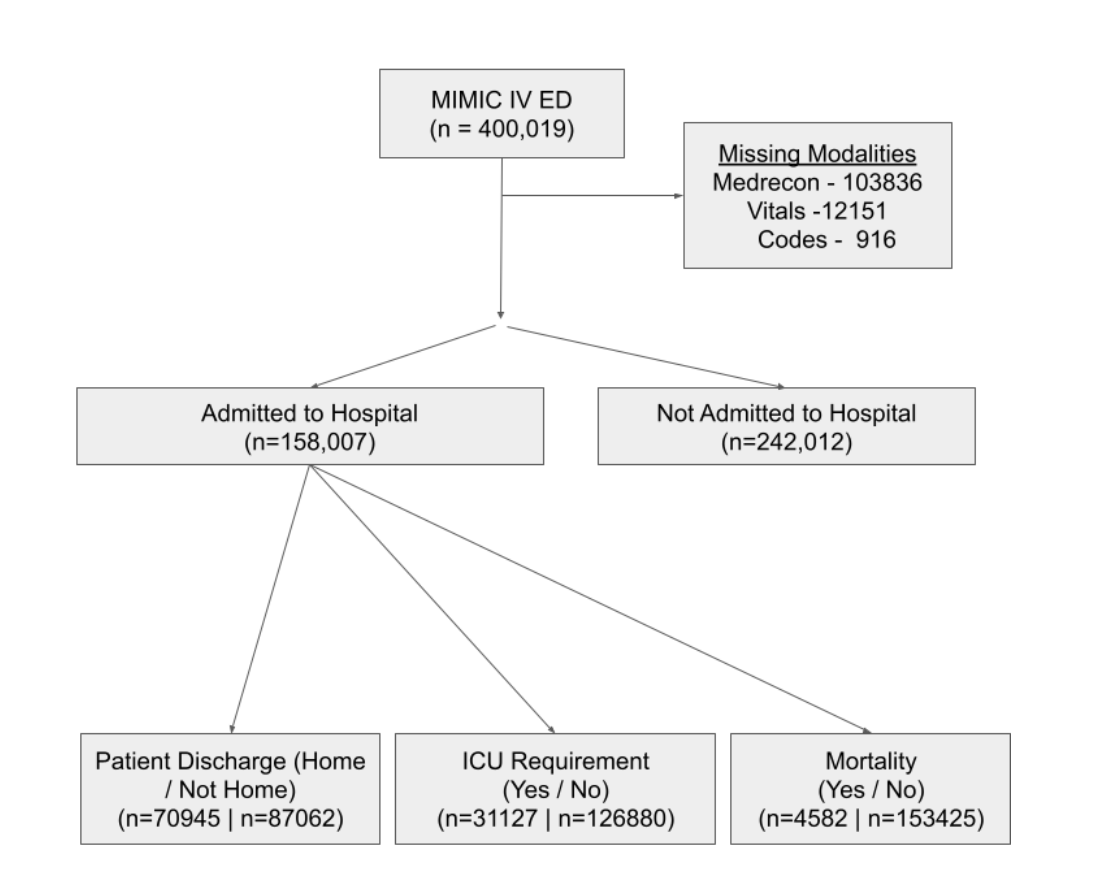
\includegraphics[width=4.5in]{plots/strobe1.png} 
   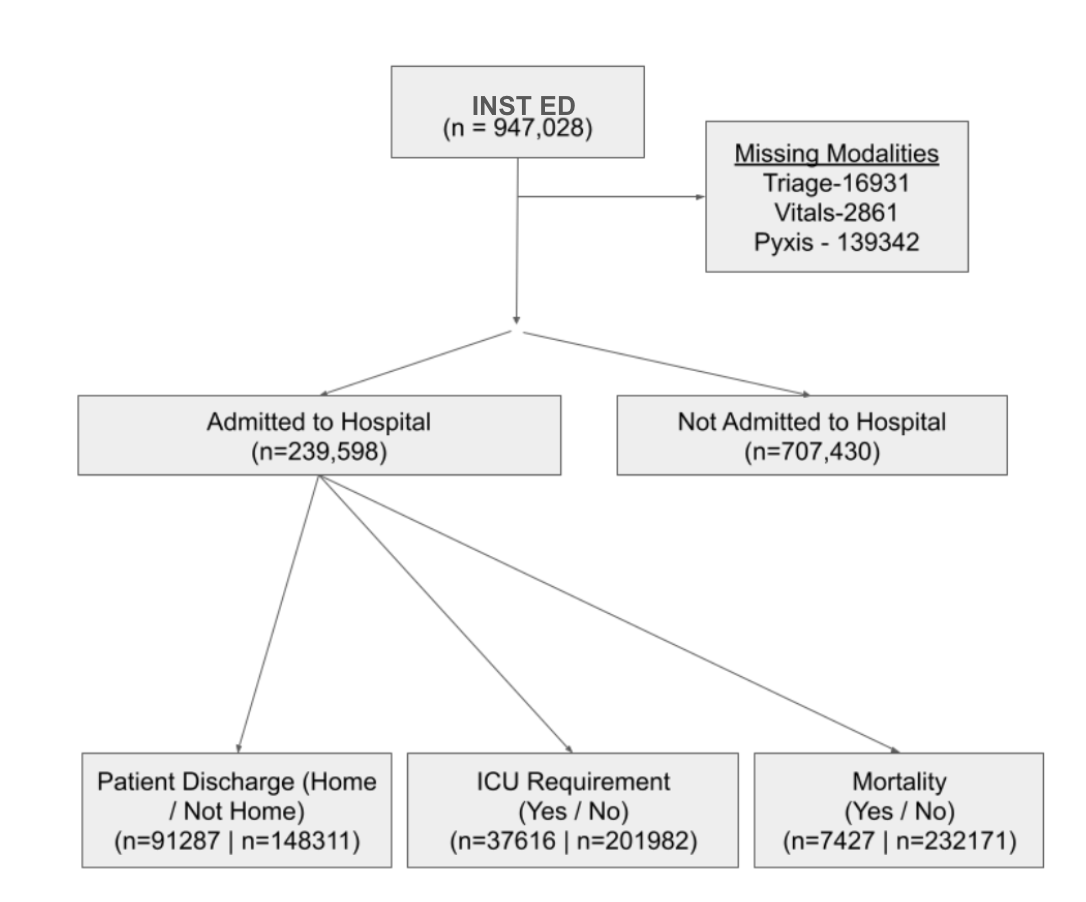
\includegraphics[width=4.5in]{plots/strobe2.png} 
   \caption{Strobe Diagrams for both MIMIC-IV ED and our Institutional ED Dataset}
   \label{strobe} 
 \end{figure} 
\newpage
\subsection{Example Pseudonotes}
\label{exnotes}

In Section \ref{notes}, we referred to the appendix to provide a verbose exploration of our pseudo-notes generation process, offering more detailed and illustrative examples. Building upon the foundation laid out earlier, we utilize color coordination to clearly delineate the  distinctions between information sourced directly from our raw EHR data and content that was dynamically generated through our script.

\begin{multicols}{2}

\textit{Arrival Information}\\
\fbox{\begin{minipage}{15em}
Patient \textcolor{red}{10000032}, a \textcolor{red}{52} year old \textcolor{red}{white female}, arrived via \textcolor{red}{ambulance} at \textcolor{red}{2180-05-06 19:17:00}. The patient's marital status is \textcolor{red}{widowed}. The patient's insurance is \textcolor{red}{other}. The patient's language is \textcolor{red}{english}.
\end{minipage}}\\

\textit{Emergency Department Disposition}\\
\fbox{\begin{minipage}{15em}
The ED disposition was \textcolor{red}{admitted} at \textcolor{red}{2180-05-06 23:30:00}. The patient died on \textcolor{red}{2180-09-09}.
\end{minipage}}\\

\textit{Triage}\\
\fbox{\begin{minipage}{15em}
At triage: temperature was \textcolor{red}{98.4}, pulse was \textcolor{red}{70}, respirations was \textcolor{red}{16}, o2 saturation was \textcolor{red}{97}, systolic blood pressure was \textcolor{red}{106}, diastolic blood pressure was \textcolor{red}{63}, pain was \textcolor{red}{0}, chief complaint was \textcolor{red}{abd pain}, \textcolor{red}{abdominal distention}. Acuity score was \textcolor{red}{3}.
\end{minipage}}\\

\textit{Medrecon}\\ 
\fbox{\begin{minipage}{15em}
The patient was previously taking the following medications: \textcolor{red}{albuterol sulfate}, \textcolor{red}{asthma/copd therapy - beta 2-adrenergic agents}, \textcolor{red}{inhaled}, \textcolor{red}{short acting}. \textcolor{red}{peg 3350-electrolytes}, \textcolor{red}{laxative - saline/osmotic mixtures}. \textcolor{red}{nicotine}, \textcolor{red}{smoking deterrents - nicotine-type}. \textcolor{red}{spironolactone [aldactone]}, \textcolor{red}{aldosterone receptor antagonists}. \textcolor{red}{emtricitabine-tenofovir [truvada]}, \textcolor{red}{antiretroviral - nucleoside and nucleotide analog rtis combinations}. \textcolor{red}{raltegravir [isentress]}, \textcolor{red}{antiretroviral - hiv-1 integrase strand transfer inhibitors}. \textcolor{red}{spironolactone [aldactone]}, \textcolor{red}{diuretic - aldosterone receptor antagonist}, \textcolor{red}{non-selective}. \textcolor{red}{furosemide, diuretic - loop}. \textcolor{red}{ipratropium bromide [atrovent hfa]}, \textcolor{red}{asthma/copd - anticholinergic agents}, \textcolor{red}{inhaled short acting}. \textcolor{red}{ergocalciferol (vitamin d2)}, \textcolor{red}{vitamins - d derivatives}.
\end{minipage}} 

\textit{Patient Vitals}\\
\fbox{\begin{minipage}{15em}
The patient had the following vitals: At \textcolor{red}{2180-05-06 23:04:00}, temperature was \textcolor{red}{97.7}, pulse was \textcolor{red}{79}, respirations was \textcolor{red}{16}, o2 saturation was \textcolor{red}{98}, systolic blood pressure was \textcolor{red}{107}, diastolic blood pressure was \textcolor{red}{60}, pain was \textcolor{red}{0}.
\end{minipage}} \\

\textit{Pyxis}\\
\fbox{\begin{minipage}{15em}
The patient received the following medications: At \textcolor{red}{2180-08-05 22:29:00}, \textcolor{red}{morphine} were administered. At \textcolor{red}{2180-08-05 22:55:00}, \textcolor{red}{donnatol (elixir), aluminum-magnesium hydrox.-simet, aluminum-magnesium hydrox.-simet, ondansetron, ondansetron} were administered. 
\end{minipage}}\\

\textit{Diagnostic Codes}\\
\fbox{\begin{minipage}{15em}
The patient received the following diagnostic codes: ICD-9 code: \textcolor{red}{[78959], other ascites}. ICD-9 code: \textcolor{red}{[07070], unspecified viral hepatitis c without hepatic coma}. ICD-9 code: \textcolor{red}{[5715], cirrhosis of liver nos}. ICD-9 code: \textcolor{red}{[v08], asymptomatic hiv infection}. 
\end{minipage}}


\end{multicols}

\subsection{Foundation Model Descriptions for Model Selection Experiment}
\label{model_des}

A Table of the foundation models that we used to select the MEME model along with their descriptions are found in Table \ref{TableModel}.

\begin{table}[H]
\centering
\caption{The foundation models evaluated for becoming the backbone for MEME.}
\begin{tabular}{p{6cm}p{8cm}}
\toprule
\textbf{Model} & \textbf{Description} \\
\midrule
\textbf{BioBERT} \citep{lee2020biobert} & A BERT variant pretrained on large biomedical corpora, enabling it to better capture domain-specific linguistic patterns and outperform general BERT on biomedical text mining tasks like named entity recognition, relation extraction, and question answering.\\
\midrule
\textbf{Bio\_ClinicalBERT} \citep{alsentzer2019publicly} & Initialized with BioBERT and further pretrained on clinical notes from the MIMIC III database (~880M words), this model is designed for tasks involving electronic health records from ICU patients.\\
\midrule
\textbf{ClinicalBERT} \citep{huang2019clinicalbert} & Pretrained on a large clinical corpus of 1.2B words spanning diverse diseases and fine-tuned on over 3 million electronic health records, this model is well-suited for clinical NLP tasks due to its understanding of medical terminology and health record data.\\
\midrule
\textbf{DistilBERT} \citep{sanh2019distilbert} & A lightweight and faster version of BERT, designed for efficient inference on resource-constrained devices while retaining most of BERT's performance on various NLP tasks.\\
\midrule
\textbf{MedBERT} \citep{9980157} & A model initialized with Bio\_ClinicalBERT and further pretrained on biomedical datasets like N2C2, BioNLP, and CRAFT, tailored for biomedical named entity recognition tasks involving diseases, drugs, genes, and other healthcare concepts.\\
\midrule
\textbf{T5} \citep{2020t5} & Pretrained on a massive text corpus using a text-to-text denoising objective, this encoder-decoder transformer model can be flexibly applied to various NLP tasks like translation, summarization, and question answering by framing them as text-to-text problems.\\
\midrule
\textbf{XLNet} \citep{yang2019xlnet} & A generalized autoregressive pretraining method that combines the advantages of autoregressive language modeling and the permutation-based approaches used in BERT. It captures bidirectional contexts by maximizing the expected likelihood over all permutations of the input sequence factorization order.\\
\bottomrule
\label{TableModel}
\end{tabular}
\end{table}

% \subsection{Model Descriptions}
% In the subsequent section, we get ino into the \iffalse intricate \fi details of the model architectures employed by other single modality approaches and \iffalse proficient \fi machine learning methods. \iffalse , offering a comprehensive exploration for pedagogical clarity. \fi We disclose more detailed hyperparameters and architectural designs that constitute these models, facilitating a transparent benchmarking process. If there are any further questions after reading this section, feel free to contact the authors for more details. \\

% \noindent\textbf{Single Modality Specific  Methods}\\
% In our analysis, we presented six distinct model variations, each tailored to one of the six modalities used for predicting the target variable. While these models share similarities with our multimodal approach, they diverge in certain aspects as deliberate feature removal sets them apart from our multimodal methodology. These single modality approaches adhere to a more conventional Language Model (LLM) fine-tuning paradigm. However they still do slightly diverge from these approaches as well. In these single modality models, we froze each LLM encoder and trained a linear classifier to be able to learn the proper underlying representations to make a proper prediction.

% Moreover, unlike our multimodal model, these single modality models forego our second step to the network, which incorporates an additional self-attention layer step, as they do not necessitate learning a unified input. This \iffalse streamlined \fi approach reflects the task-specific focus of these models, optimizing for individual modality predictions without the need for a unified multimodal analysis.

% In terms of preprocessing, we used the same preprocessing steps as our multimodal approach and extracted the modality-specific subset Dataset object from the Hugging Face library for our analysis. Subsequently, we loaded these dataset objects into conventional PyTorch dataloaders for training the classifier. Similar to our multimodal approach, we also utilized the Cross-Entropy Loss and AdamW optimizer, with a learning rate of $5e-5$, and trained until the validation error converges. Additionally, we implemented a linear learning rate scheduler to adjust the model’s learning rate during training, thus tuning this hyperparameter, which impacts our overall model performance. We tracked F1 scores to assess the performance of our model after every epoch. \\ 

% \noindent\textbf{Multimodal Single Embedding Model}\\
% In our benchmarking study, we also included a model referred to as the Multimodal Single Embedding Model (MSEM). This inclusion represents the canonical LLM approach of \iffalse aimed to preemptively address potential queries about \fi consolidating all text data into a single embedding. The MSEM closely resembles single modality models in terms of architecture; however, it diverges primarily in its preprocessing step, where all text is merged into a single column and truncated during tokenization.

% The feasibility of an MSEM is largely constrained by context-length limitations imposed by BERT and other Large Language Models (LLMs). In our study, we focused on Emergency department EHR data, which encompassed six corresponding modalities. However, in broader applications like general EHR, the data can span as many as 10-20 different modalities related to a patient's health history. These limitations are significant as they potentially restrict the depth and breadth of data that can be effectively processed and analyzed by models like the MSEM. \\

% \noindent\textbf{Random Forest Classifier}\\
% Lastly, our benchmarking also involved training and fitting a Random Forest classifier. \iffalse Renowned as an ensemble learning technique, Random Forest is part of the decision tree-based algorithm family. Its strength lies in constructing multiple decision trees whose collective outputs are aggregated to yield predictions that are both robust and accurate. \fi We selected 1000 estimators, equivalent to creating 1000 trees. \iffalse Given our ample resources, handling this substantial number of estimators was feasible, thus influencing our choice of this particular hyperparameter. \fi 
% In contrast to our approach with pseudo-notes, the data preparation for the Random Forest classifier was markedly different. While BERT and transformer-based models primarily process text data, such an approach was not viable with the Random Forest. Consequently, we utilized the EHR data in its unaltered tabular format. To maintain consistency across our analyses, we filtered this data using the same patient subsets identified in the test, validation, and training sets of our transformer-based methods. Furthermore, we implemented one-hot encoding on various modalities, including medication reconciliation, ICD codes, and Pyxis drugs, to effectively prepare the data for the Random Forest model.

\newpage
\subsection{Ablation Study Table}
\label{ablation}

We display the raw performance metrics from our ablation study of the various modalities contributing to the multiple tasks proposed in our work on the MIMIC IV ED dataset. The complete set of results is displayed in Tables \ref{r4}, \ref{r5}, \ref{r6}}. We note that no modality alone beat out the MEME model which took on a multimodal approach. 

\begin{table}[h!]
\centering
\caption{F1 Scores for MIMIC-IV ED Dataset Ablation Study Across Different Tasks.}
\label{r4}
\begin{adjustbox}{width=5in}
\begin{small}
\begin{sc}
\begin{tabular}{l|c|ccc}
\toprule
F1 Benchmark & Dispositon & & Decompensation &\\
Modality & ED Disposition & Discharge & ICU & Mortality \\
\midrule
Arrival & 0.895 $\pm$ 0.003 & 0.533 $\pm$ 0.008 & 0.041 $\pm$ 0.009 & 0.063 $\pm$ 0.005 \\
Codes & 0.613 $\pm$ 0.003 & 0.572 $\pm$ 0.008 & 0.054 $\pm$ 0.009 & 0.055 $\pm$ 0.004 \\
Medrecon & 0.625 $\pm$ 0.005 & 0.525 $\pm$ 0.009 & 0.029 $\pm$ 0.005 & 0.054 $\pm$ 0.004 \\
Pyxis & 0.564 $\pm$ 0.004 & 0.478 $\pm$ 0.009 & 0.167 $\pm$ 0.015 & 0.060 $\pm$ 0.005 \\
Triage & 0.596 $\pm$ 0.005 & 0.403 $\pm$ 0.010 & 0.367 $\pm$ 0.015 & 0.055 $\pm$ 0.004 \\
Vitals & 0.619 $\pm$ 0.005 & 0.366 $\pm$ 0.009 & 0.160 $\pm$ 0.013 & 0.067 $\pm$ 0.006 \\
MEME & \textbf{0.943 $\pm$ 0.003} & \textbf{0.698 $\pm$ 0.007} & \textbf{0.572 $\pm$ 0.014} & \textbf{0.137 $\pm$ 0.035} \\
\bottomrule
\end{tabular}
\end{sc}
\end{small}
\end{adjustbox}
\end{table}

\begin{table}[H]
\caption{AUROC Scores for MIMIC-IV ED Dataset Ablation Study Across Different Tasks.
}
\centering
\label{r5}
\begin{adjustbox}{width=5in}
\begin{small}
\begin{tabular}{l|c|ccc}
\toprule
AUROC Benchmark & Dispositon & & Decompensation &\\
Modality & ED Disposition & Discharge & ICU & Mortality \\
\midrule
Arrival & 0.940 $\pm$ 0.002 & 0.689 $\pm$ 0.007 & 0.682 $\pm$ 0.009 & 0.709 $\pm$ 0.019 \\
Codes & 0.715 $\pm$ 0.005 & 0.658 $\pm$ 0.007 & 0.714 $\pm$ 0.008 & 0.709 $\pm$ 0.020 \\
Medrecon & 0.709 $\pm$ 0.004 & 0.644 $\pm$ 0.007 & 0.622 $\pm$ 0.009 & 0.668 $\pm$ 0.021 \\
Pyxis & 0.498 $\pm$ 0.005 & 0.616 $\pm$ 0.008 & 0.704 $\pm$ 0.009 & 0.705 $\pm$ 0.024 \\
Triage & 0.677 $\pm$ 0.004 & 0.647 $\pm$ 0.007 & 0.758 $\pm$ 0.008 & 0.736 $\pm$ 0.020 \\
Vitals & 0.720 $\pm$ 0.004 & 0.598 $\pm$ 0.008 & 0.733 $\pm$ 0.008 & 0.740 $\pm$ 0.021 \\
MEME & \textbf{0.991 $\pm$ 0.001} & 0.\textbf{799 $\pm$ 0.006} & \textbf{0.870 $\pm$ 0.015} & \textbf{0.862 $\pm$ 0.006} \\
\bottomrule
\end{tabular}
\end{small}
\end{adjustbox}
\end{table}

\begin{table}[H]
\centering
\caption{AUPRC Scores for MIMIC-IV ED Dataset Ablation Study Across Different Tasks.}
\label{r6}
\begin{adjustbox}{width=5in}
\begin{small}
\begin{tabular}{l|c|ccc}
\toprule
AUPRC Benchmark & Dispositon & & Decompensation &\\
Model & ED Disposition & Discharge & ICU & Mortality \\
\midrule
Arrival & 0.861 $\pm$ 0.005 & 0.625 $\pm$ 0.010 & 0.376 $\pm$ 0.014 & 0.076 $\pm$ 0.013 \\
Codes & 0.645 $\pm$ 0.007 & 0.595 $\pm$ 0.011 & 0.410 $\pm$ 0.014 & 0.061 $\pm$ 0.008 \\
Medrecon & 0.589 $\pm$ 0.007 & 0.579 $\pm$ 0.010 & 0.286 $\pm$ 0.010 & 0.049 $\pm$ 0.006 \\
Pyxis & 0.391 $\pm$ 0.005 & 0.561 $\pm$ 0.011 & 0.484 $\pm$ 0.015 & 0.112 $\pm$ 0.022 \\
Triage & 0.552 $\pm$ 0.008 & 0.579 $\pm$ 0.011 & 0.504 $\pm$ 0.015 & 0.100 $\pm$ 0.017 \\
Vitals & 0.623 $\pm$ 0.007 & 0.544 $\pm$ 0.010 & 0.430 $\pm$ 0.014 & 0.087 $\pm$ 0.014 \\
MEME & \textbf{0.983 $\pm$ 0.002} & \textbf{0.765 $\pm$ 0.008} & \textbf{0.709 $\pm$ 0.012} & \textbf{0.243 $\pm$ 0.034} \\

\bottomrule
\end{tabular}
\end{small}
\end{adjustbox}
\end{table}
\newpage
\subsection{GPT3.5-Turbo Prompt}
\label{gptee}

\begin{lstlisting}[language=Python, caption=Basic Example of How prompted the gpt-3.5-turbo model to generate predictions.]
from openai import OpenAI
client = OpenAI()

completion = client.chat.completions.create(
  model="gpt-3.5-turbo",
  messages=[
    {"role": "system", "content": "You are a medical officer, skilled in determining whether a patient should be admitted to the Emergency Room or not."},
    {"role": "user", "content": "I have 10 patient samples here. I need you to predict whether each patient should be admitted to the emergency room or not. Give you prediction in the list format ([`1,0,0,1,1,1,0,1,0,1']) and predict 1 if they should be admitted and 0 if not:\n\n'Patient 10000032, a 52 year old white female, arrived via ambulance at 2180-05-06 19:17:00. The patient's marital status is widowed. The patient's insurance is other. The patient's language is english.The patient received the following diagnostic codes: ICD-9 code: [5728], oth sequela, chr liv dis. ICD-9 code: [78959], other ascites. ICD-9 code: [07070], unspecified viral hepatitis c without hepatic coma. ICD-9 code: [v08]...'

    ...
    [OTHER_PSEUDONOTES]
    ...
    "}
  ]
)

print(completion.choices[0].message)

>>> Here are the predictions: {"predictions": [1, 0, 1, 1, 1, 1, 1, 1, 1, 1]}
\end{lstlisting}

We conducted a benchmarking study comparing whether training a model was necessary with the emergence of generative AI like (GPT, LLaMA, etc.). Here, we present a bar graph of the performance of MEME relative to prompting based approach. We find that training a classifier remains preferable.

\begin{figure}[h!]
    \centering
    \includegraphics[width=3in]{plots/dispo.png}
    \caption{Comparison of Classification Accuracies: Training a Classifier (MEME) versus Utilizing a Generative Model (GPT-3.5-Turbo) for Prediction}
    \label{gpt-meme}
\end{figure}


\subsection{Why did Generalization Fail?}
\label{gener3}

% \begin{figure}[h!] 
%     \centering
%     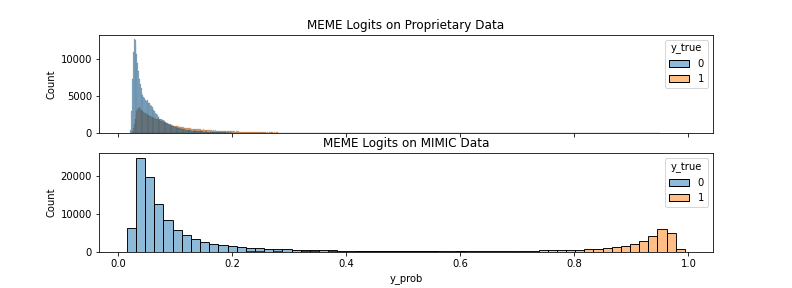
\includegraphics[width=\columnwidth]{logits.png}
%     \caption{The Logits Generated from Running MEME on MIMIC IV versus Institutional Dataset}
%     \label{fig:enter-label}
% \end{figure}

To investigate the failure of our generalization experiment from MIMIC to our institutional database, we conducted a thorough examination of the data input into our pseudo-notes method. We analyzed the data from both Electronic Health Record (EHR) sources by plotting distributions via box plots, and Venn diagrams to elucidate the disparities between the datasets.

\subsubsection*{Arrival Information}

All results related to \textit{arrival} information are presented in Figure \ref{app1}. We observe notable differences within these extensive categorical classes for arrival transport and race labels. Although these differences are not considered substantial, highlighting these disparities remains critical.

\begin{figure}[h!]
   \centering 
   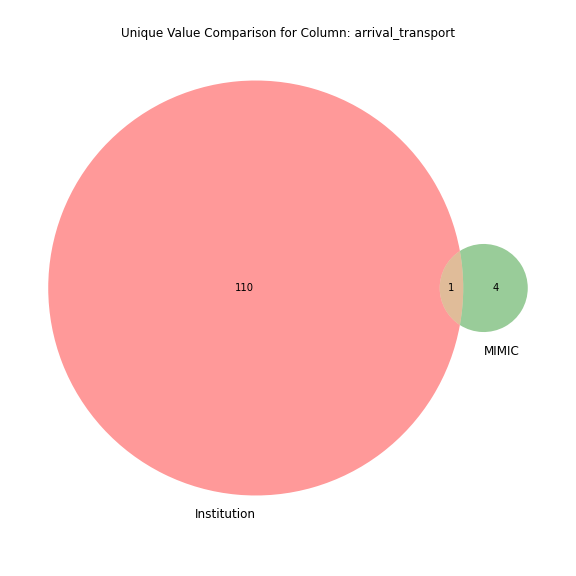
\includegraphics[width=4.5in]{plots/arrival_transport_venn.png} 
   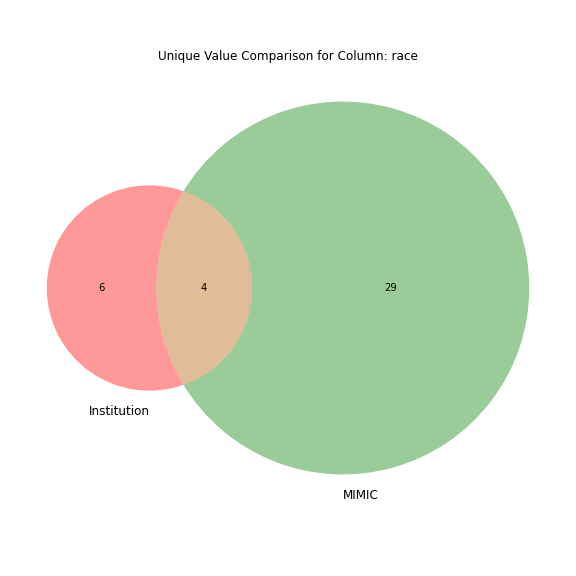
\includegraphics[width=4.5in]{plots/race_venn.png} 
   \caption{The Venn diagram illustrates the overlap between unique elements identified in our Institutional Data and MIMIC-IV ED \textbf{Arrival} Information Data.}
   \label{app1} 
 \end{figure} 

 \subsubsection*{Diagnoses}
All results pertaining to \textit{diagnoses }information are presented in Figure \ref{app2}. We observe notable differences within the ICD Diagnostic codes. These differences are critical and may contribute to failed generalization.
 
 \begin{figure}[h!]
   \centering 
   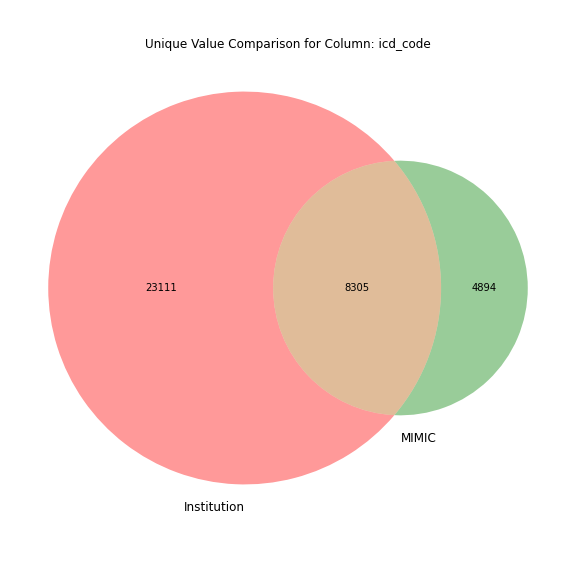
\includegraphics[width=4.5in]{plots/icd_code_venn.png} 
   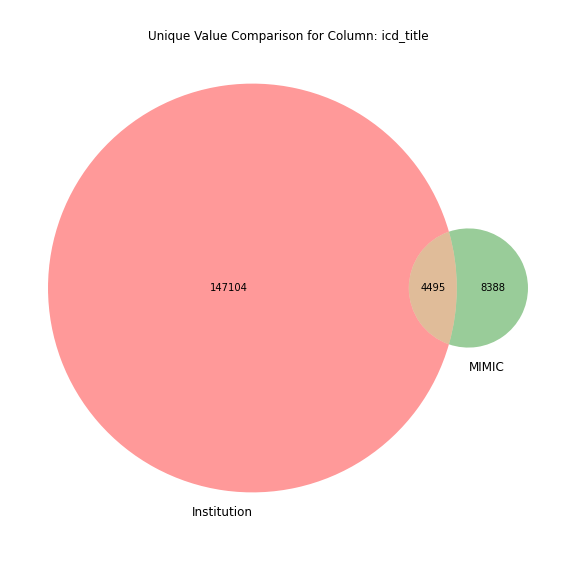
\includegraphics[width=4.5in]{plots/icd_title_venn.png} 
   \caption{The Venn diagram illustrates the overlap between unique elements identified in our Institutional Data and MIMIC-IV ED \textbf{Diagnoses} Data.}
   \label{app2} 
 \end{figure} 

 \subsubsection*{Pyxis}
 All results pertaining to \textit{pyxis} information are presented in Figure \ref{app3}. We observe notable differences within the drug names dispensed during their ED Visit. These differences are critical and may contribute to failed generalization.
 \begin{figure}[h!]
   \centering 
   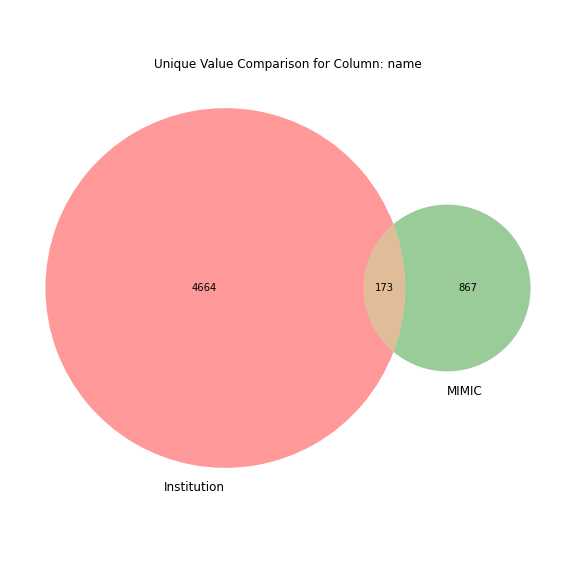
\includegraphics[width=5in]{plots/name_venn.png} 
   \caption{The Venn diagram illustrates the overlap between unique elements identified in our Institutional Data and MIMIC-IV ED \textbf{Pyxis} Data.}
   \label{app3} 
 \end{figure} 

 \subsubsection*{Triage}
All results related to \textit{pyxis} information are presented in Figures \ref{app4} and \ref{app5}. We observe notable differences in the chief complaints, which were anticipated to vary. However, we emphasize that numerical values within EHRs appeared as expected and exhibited similar distributions with marginal outliers. These differences are critical and may contribute to failed generalization.

\begin{figure}[h!]
   \centering 
   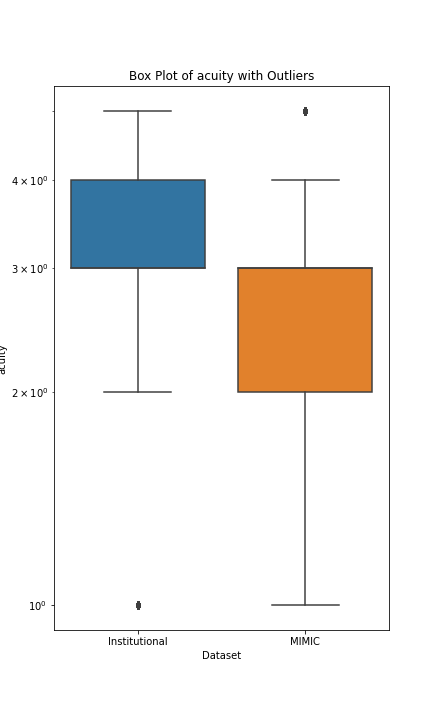
\includegraphics[width=2.5in]{plots/acuity_triage_boxplot.png} 
   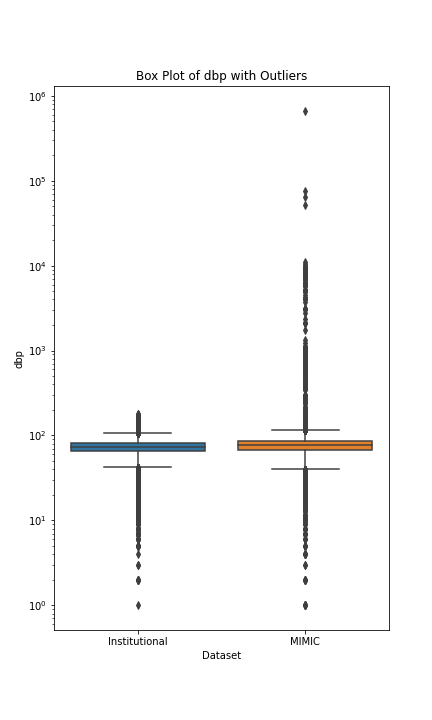
\includegraphics[width=2.5in]{plots/dbp_triage_boxplot.png} 
   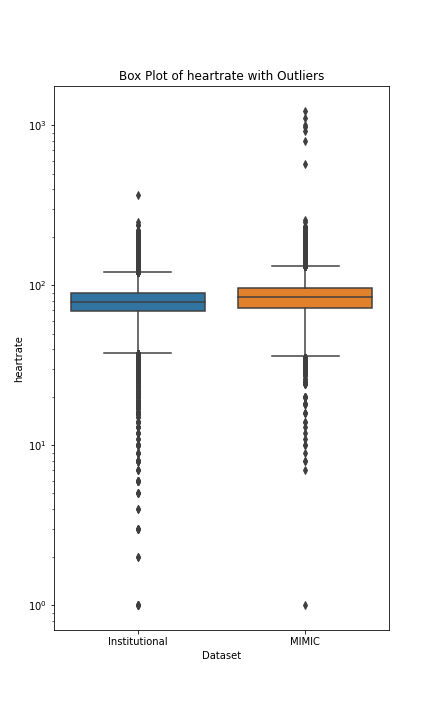
\includegraphics[width=2.5in]{plots/heartrate_triage_boxplot.png} 
   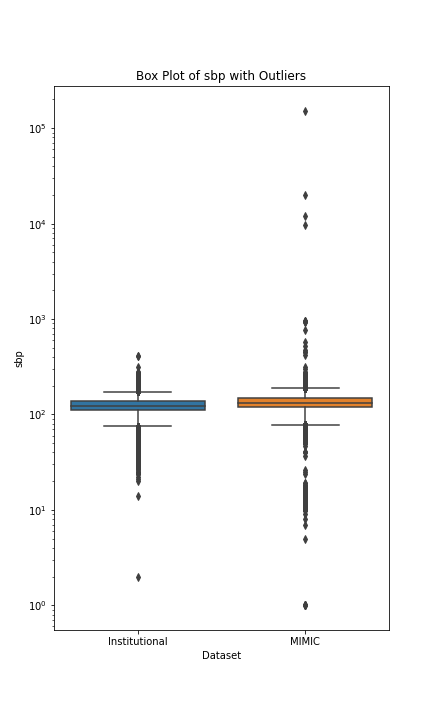
\includegraphics[width=2.5in]{plots/sbp_triage_boxplot.png} 
   \caption{The box plot depicts the distribution of values within Institutional and MIMIC-IV ED \textbf{Triage Information} Datasets, thereby facilitating a comparative analysis of data variability and central tendency across the datasets.}
   \label{app4} 
 \end{figure} 

 \begin{figure}[h!]
   \centering 
   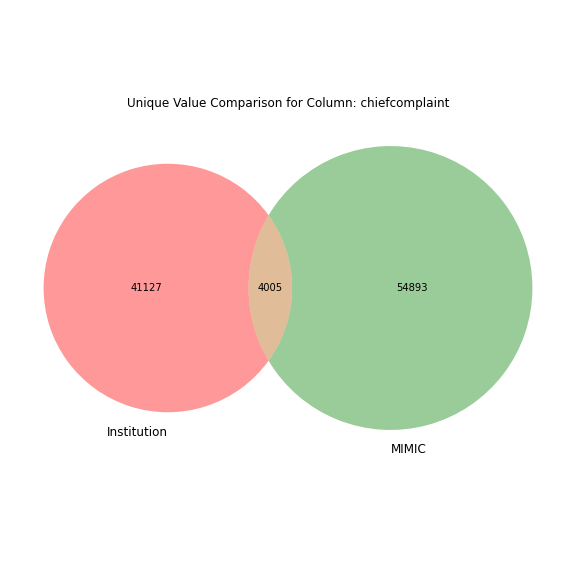
\includegraphics[width=5in]{plots/chiefcomplaint_venn.png} 
   \caption{The Venn diagram illustrates the overlap between unique elements identified in our Institutional Data and MIMIC-IV ED \textbf{Chief Complaints} Data coming from \textbf{Triage} Information.}
   \label{app5} 
 \end{figure} 

 \subsubsection*{Vitals}
All results related to \textit{vitals} information are presented in Figures \ref{app6}. We see again that numerical data appears to follow similar distributions despite a few outliers. We do not think the numerical aspects of the EHR led to failed generalization.
\begin{figure}[h!]
   \centering 
   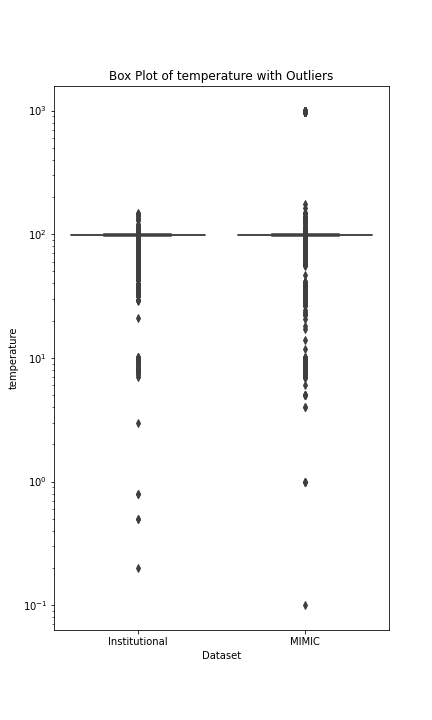
\includegraphics[width=2.5in]{plots/temperature_boxplot.png} 
   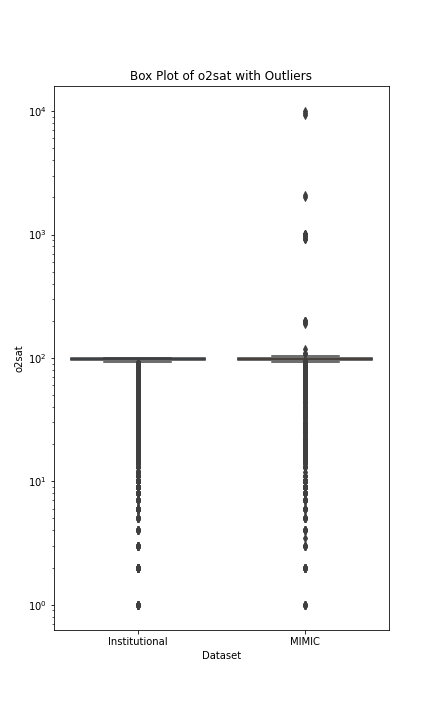
\includegraphics[width=2.5in]{plots/o2sat_boxplot.png} 
   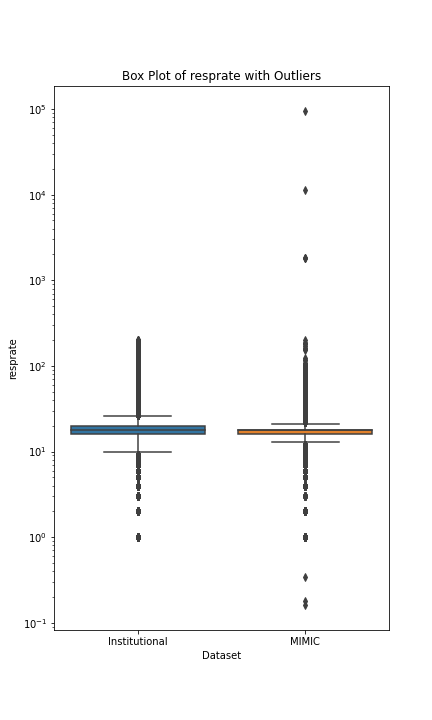
\includegraphics[width=2.5in]{plots/resprate_boxplot.png} 
   \caption{The box plot depicts the distribution of values within Institutional and MIMIC-IV ED \textbf{Vitals Information} Datasets, thereby facilitating a comparative analysis of data variability and central tendency across the datasets.}
   \label{app6} 
 \end{figure} 

\subsection*{Remarks based on Analysis}

Our analysis reveals that EHR systems exhibit significant variability especially in the case of free text and categorical data types. This diversity is evident in the unique chief complaints, diagnostic annotations, and other unique medical cases of different hospital institutions, which contribute to the challenges in achieving generalization. These insights underscore the complexities inherent in working across heterogeneous EHR environments and advise to use this method with some local fine-tuning of hospitals as highlighted in \citep{jiang2023health}.
\end{document}
% \section{Introduction}

% In recent years, increased access to Electronic Health Records (EHR) has \iffalse emerged as pivotal sources of data, burgeoning with \fi provided patients and healthcare systems with valuable insights into a patient's health history. This wealth of information makes EHR indispensable for inference tasks, particularly as the machine learning community increasingly focuses on healthcare applications. Both traditional and cutting-edge machine learning techniques have been harnessed to aid in specific diagnosis and prognosis tasks \citep{shickel_deep_2018}, with a recent keen interest in incorporating state-of-the-art language models, such as Large Language Models (LLMs) \citep{zhao_survey_2023}. These advanced models, which have been pre-trained on extensive and diverse textual corpora, bring a broad understanding across numerous domains, thereby significantly enhancing their adaptability and effectiveness for a variety of complex tasks. Particularly noteworthy is their ability to generate high-fidelity latent representations \iffalse high-dimensional representational vector embeddings \fi, which can be directly employed in many classification tasks, often demonstrating state-of-the-art performance. However, the adoption of these models, built for natural language and text, has been hampered by the fact that the canonical form of generally available EHR data is tabular, and access to textual clinical notes are generally infeasible to access due to privacy concerns. 

% Therefore, in this work, we introduce \textit{Multiple Embedding Model for EHR (MEME)}, an approach that processes \iffalse multimodal \fi tabular health records \iffalse data \fi and generates textual representations. \iffalse from it, forming the foundation for  (clinical pseudo-notes) \fi Using these clinical pseudo-notes, MEME \iffalse transcends the limitations of traditional EHR data usage by transforming structured data into a format conducive to modern NLP techniques through our ``pseudo-notes'' generation, effectively bridging \fi bridges the gap between tabular EHR data and modern NLP techniques. \iffalse textual classification. \fi We then demonstrate the effectiveness of this approach by showcasing it on various EHR prediction tasks related to the Emergency Department (ED) across multiple hospital institutions. \iffalse Despite the straightforward and simple formulation of our method, we \fi We also find that adopting a multimodal strategy, where different components of the EHR are encoded separately, yields better results compared to the single modality embedding approach, Multimodal Single Embedding Model (MSEM), and other conventional machine learning methodologies.  \iffalse and thereby inspiring the method's name. \fi

% \subsection{Contributions}

% \begin{figure*}[h!]
% \vskip 0.2in
% \begin{center}
% \label{model}
% \centerline{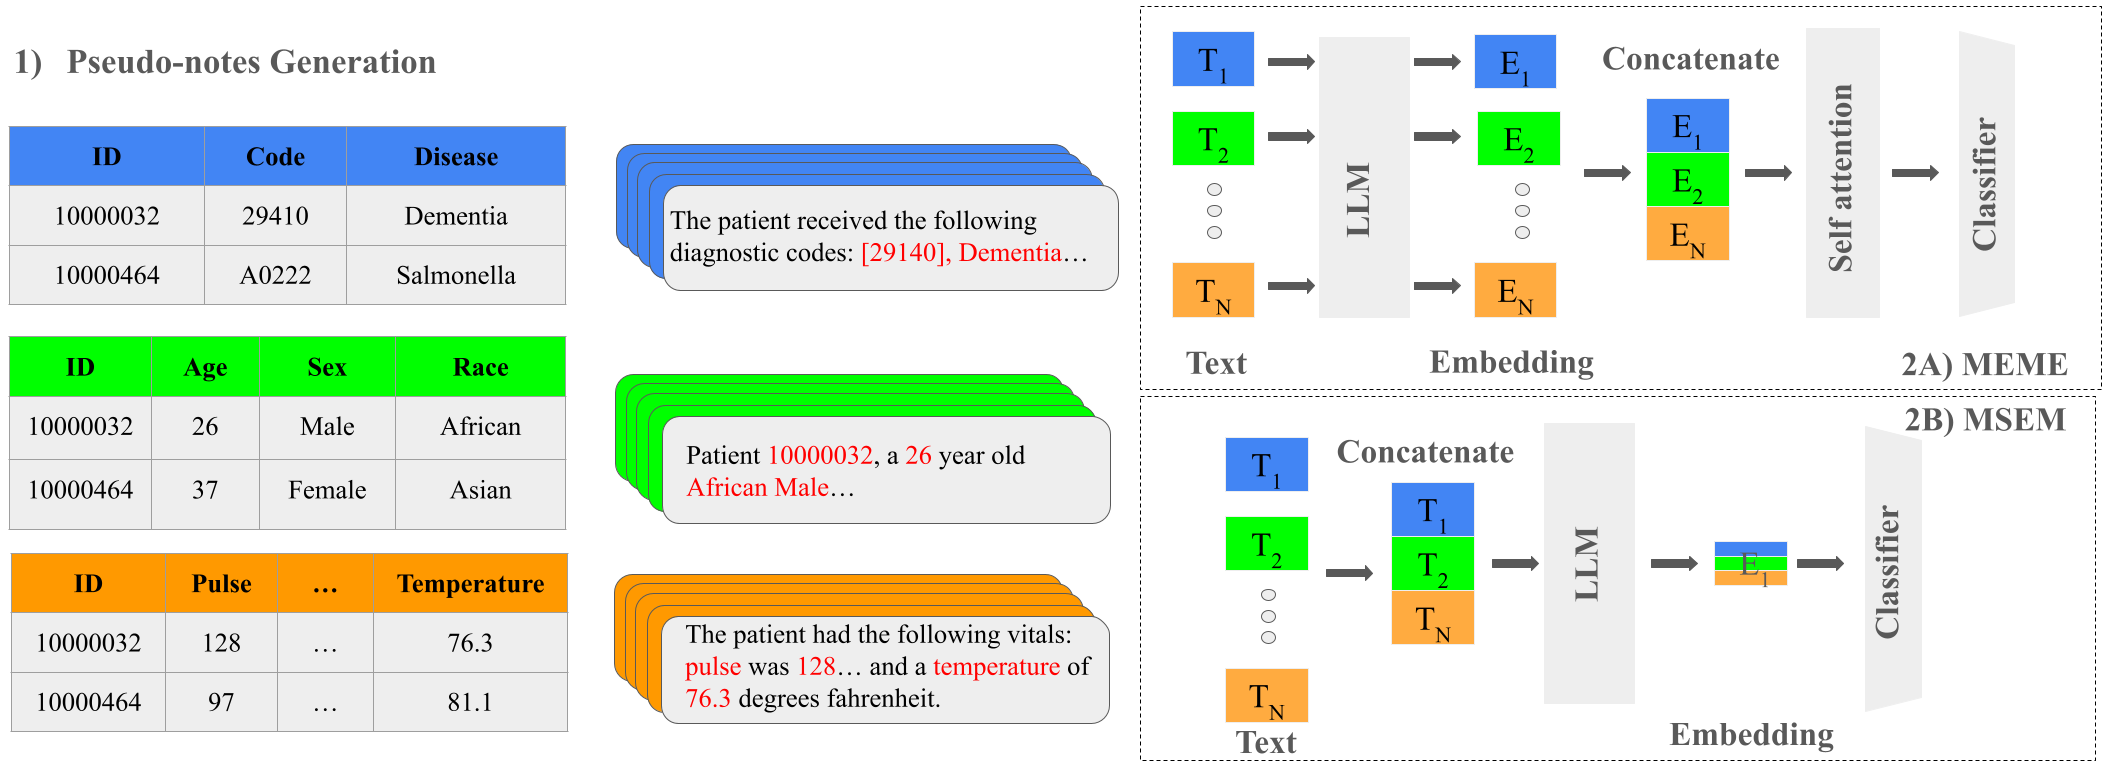
\includegraphics[width=0.99\textwidth]{figures/model.png}}
% \caption{We graphically represent the Pseudo-notes method (1) alongside the architecture of the Multiple Embedding Model for Electronic Health Records (MEME), as well as that of its counterpart, the Multimodal Single Embedding Model (MSEM). We display both models to highlight the subtle differences between the two approaches, noting that MSEM adheres to a more conventional methodology as demonstrated by other research groups. }
% \label{model-2}
% \end{center}
% \vskip -0.2in
% \end{figure*}

% The main contributions of this work are as follows:
% \begin{itemize}
%     \item We introduce our method \textit{MEME}, a novel approach that converts \iffalse multimodal \fi tabular EHR data into clinical pseudo-notes. These notes are designed to be utilized in a variety of EHR-related tasks and were developed in collaboration with a clinician informaticist, drawing inspiration from patient report generation tools. \iffalse s generated by auto-complete systems.\fi
%     \item We demonstrate that multimodal representation outperforms traditional machine learning and LLM-based models which represent EHR as a single heterogeneous data modality \iffalse We test the effectiveness of this model by applying this textual representation of EHR to various Emergency Department prediction tasks, showcasing strong performance \fi across multiple tasks.
%     \item We find that the representation derived from the MIMIC-IV Database is insufficient for generalizing across different hospital systems.
% \end{itemize}

% \section{Related Work}

% \subsection{LLM \& Tabular Data}

% An ongoing field of research involves the application of LLMs to tabular data. Previous attempts at constructing representations for tabular data have led to the emergence of a novel concept known as “stringified” or serialized tabular data. This technique involves converting tabular data into a text-based format, either as a simplified list (e.g., Age: 42, Height: 143cm, ...) or as serialized sentences. This transformation enables a more natural integration of diverse data types into language models, facilitating their analysis using advanced machine learning techniques.

% This growing interest has enabled the application of state-of-the-art language models to tabular data, often surpassing traditional machine learning models in scenarios with minimal or no training data. Such capability was demonstrated through a text-to-text prompt-based method using serialized tabular data, leveraging the general knowledge embedded within the parameters of LLMs across various zero-shot and few-shot learning tasks \cite{hegselmann2023tabllm}.  Moreover, another study explored the integration of paired datasets (e.g., images) for game data, incorporating both tabular textual and visual fields cohesively for predictive tasks. This was achieved using BERT models to handle the textual component of the datasets \cite{lu2023MuG}, showcasing their versatility in processing complex data structures and blending different types of information seamlessly. Such integrative approaches suggest new possibilities in applying LLMs beyond traditional text-based applications.

% \subsection{LLMs, Transformers \& EHR}
% Transformer based models and LLMs have also been increasingly applied to EHR data \citep{kalyan_ammu_2022}. These applications tend to fit in one of two paradigms as identified by \citep{wornow_shaky_2023}: One approach that operates upon structured information captured within the EHR and another that operates upon clinical text with recent methods involving multimodal approaches. 

% The models developed to represent structured EHR are generally based on the BERT architecture \citep{kalyan_ammu_2022}. Broadly speaking, these approaches represent the electronic health record as a sequence of events. For example, BEHRT and its derivatives MedBert, CEHR-Bert, construct sequences of diagnostic codes and visit metainformation to be compatible with the BERT framework \citep{li_behrt_2020, li_hi-behrt_2021, rasmy_med-bert_2021, pang_cehr-bert_nodate}. These models are better adapted to currently available healthcare data due to deidentification and standardization efforts (e.g., OHDSI/OMOP \citep{noauthor_omop_nodate}). Notably, nearly all approaches treat EHR data as a single heterogeneous data source, despite the fact that EHR covers data across multiple biological scales and clinical domains (e.g., billing-related diagnostic codes, molecular blood tests, vital-sign measurements). \iffalse embedding. By treating EHR as a single embedding, they are able to represent the patient's health trajectory comprehensively. However, \fi Indeed, more recently, EXBEHRT found that separately representing the components of EHR offers several benefits, including improved performance, shortened sequence length, and fewer required parameters \citep{rupp_exbehrt_2023}. 
% %This shift towards multi-modality also addresses the current models' inability to work with missing data and provides a more nuanced understanding of a patient’s health profile.

% Another approach directly operates upon clinical notes, which are in the form of natural text. The primary advantage of these approaches is the ability to incorporate pretrained models, such as GPT, BioBert, PubMedBert, etc. \citep{roy-pan-2021-incorporating, chief-bert}. However, these data are challenging to acquire, with nearly all applications restricted to a single database (MIMIC-III, \citep{johnson_mimic-iii_2016}). Recently, efforts have been made to begin multimodal analysis, where groups analyze different data from the EHR (imaging, waveforms, etc.) for predictive tasks. MC-BEC uses all available data within their in-house dataset and performs a multilabel classification on various EHR tasks \citep{chen2023multimodal}. Other attempts have unified imaging data with text \citep{khader2023medical}, and imaging data with structured EHR for various analyses \citep{zhou2023transformer}.

% Therefore, in this work, with the continued development of multimodal transformer and LLM methods, we develop our own approach that can capture a joint representation of multimodal structured EHR data. We do so by constructing ``pseudo-notes" out of raw EHR tabular data contained within the MIMIC-IV and institutional datasets. We then feed this data into a feed forward network with self attention to train a classifier model to predict various binary classification tasks related to the emergency department. This approach allows us to compare single-modality, MSEM and multi-modality approaches and assess performance on this transformer method.

% \section{Benchmarks}
% \label{data}
% \subsection{Benchmark tasks}

% This paper focuses on binary prediction tasks around Emergency Department disposition and decompensation defined in \cite{chen2023multimodal}. \iffalse EHR ED Prediction, utilizing EHR ED data to anticipate class labels for various downstream binary classification tasks. \fi We test our multimodal method's ability to be used in both single classification and multilabel classification tasks benchmarked against other single modality and traditional machine learning models. This assessment aims to demonstrate the performance advantages of adopting a multimodal strategy.

% \begin{enumerate}
%         \item \textbf{ED Disposition (Binary Classification):} Our first objective is to predict ED Disposition, determining where patients were sent after their Emergency Room visit, based on EHR measurements recorded during their stay in the ED. We frame this as a binary classification problem, distinguishing whether the patient was discharged home or admitted to the hospital.
        
%         \item \textbf{ED Decompensation} \iffalse Tasks \fi (Multilabel Binary Classification): Our subsequent objective is to analyze the subset of patients admitted to the hospital and predict various other measures related to the ED. In this set of tasks, we adopt a multilabel binary classification approach, where the model predicts three separate ED tasks simultaneously. The first task involves predicting the patient's next discharge location, distinguishing between home and other facilities (not home). The second task is predicting the requirement for Intensive Care Unit (ICU) admission.
%         And the last task
%         is predicting patient mortality, specifically whether the patient dies during their 
%         hospital stay.  
% \end{enumerate}

% \begin{table}[h!]
% \caption{Prevalence Statistics for Different Benchmark Tasks in the MIMIC-IV and Institutional Datasets}
% \label{prevalence-table}
% \vskip 0.15in
% \begin{center}
% \begin{small}
% \begin{sc}
% \begin{tabular}{lcc}
% \toprule
% Task & MIMIC-IV & Institutional \\
% \midrule
% ED Disposition & 0.395 & 0.253 \\
% \bottomrule
% Discharge Location & 0.449 & 0.381 \\
% ICU & 0.197 & 0.157 \\
% Mortality & 0.029 & 0.031 \\
% \bottomrule
% \end{tabular}
% \end{sc}
% \end{small}
% \end{center}
% \vskip -0.1in
% \end{table}

%  In Table \ref{prevalence-table}, we detail the classification objectives and provide a summary of dataset statistics related to the prevalence of each label in these tasks.

% \subsection{Data Source}
% % EHR data are heterogeneous, spanning multiple data types and multiple biological domains and scales
% % we address the multiple data types by converting to text. we address multiple biological domains and scales as multimodal.

% Our study sources data from the Medical Information Mart for Intensive Care (MIMIC)-IV v2.2 database \citep{johnson_mimic-iv_nodate} and our institutional EHR database. We detail the components of these databases to further explore the data inputs for our model. The use of these diverse databases allows for \iffalse a comprehensive \fi examination of EHR data across different settings and patient populations, enhancing the generalizability of our findings.

% \begin{itemize}
%     \item \textbf{MIMIC-IV:} For these downstream tasks, the EHR concepts (modalities) utilized include: \textit{arrival information}, capturing patient demographics and means of arrival; \textit{triage}, documenting patient vitals and complaints at the time of arrival; \textit{medication reconciliation (medrecon)}, detailing prior and current medications taken by the patient; \textit{diagnostic codes} (ICD-9/10 codes) assigned for diagnosis; as well as measurements collected throughout the ED stay, including \textit{patient vitals} and medications received from \textit{pyxis}. All data points across modalities can be combined using a unique Visit or Hospital admission ID (Hadm\_id) and can also be connected to all prediction labels. 
    
%     \item \textbf{Institutional Database:} 
%     In our institutional data, we have access to all data modalities from the MIMIC-IV database, with the exception of medication reconciliation (medrecon). However, there may be slight variations in the data across modalities due to the lack of certain features in different EHR systems. Our approach is to model our pseudo-notes so that they closely resemble each other. Similar to the MIMIC-IV database, all modalities in our institutional data can be linked using a hospital admission ID and are also associated with all prediction labels.

% \end{itemize}

% In the MIMIC-IV database, we analyzed $400,019$ patients, each associated with six modalities, contributing to a dataset size of approximately $2.4$ million text paragraphs. For predicting ED Disposition, we use the available data for training, validation, and testing with a set seed for reproducibility purposes. For the three decompensation prediction tasks, \iffalse next three binary multiclass classification tasks, \fi we utilize the subset of patients who were admitted to the hospital from the ED, \iffalse Disposition task, \fi resulting in a sample size of $158,010$ patients.

% Additionally, in the Institutional database, we have a much larger sample size of $947,028$ patients with 5 available modalities (excluding \textit{medrecon}, \iffalse and 1 filler modality (missing medrecon), \fi resulting in approximately $4.75$ million text paragraphs derived from the EHR. We use all available data for the ED disposition task, and the $240,161$ admitted patients were used for decompensation prediction. \iffalse s and reduce the number again for the multilabel classification, resulting in $240,161$ patients. \fi 
% % In the appendix, we include a STROBE Diagram to provide a more organized data breakdown, offering a clear visual representation of the patient flow and data utilization in our study.

% % In addition to this dataset description, to ascertain the effectiveness of the multimodal approach, we assess the similarities between the six modalities by calculating the average pairwise mutual information scores. This metric reveals that no modality exceeds a 10\% mutual information score, indicating that there is hardly any overlap between these vector representations across all modalities. This implys the potential of leveraging multiple independent information sources for enhanced predictive capabilities.

% \section{Methods}

% % The core components of MEME are the development of pseudo-notes and multimodal handling of EHR data. 
% % We validate it against SOTA benchmarks within and across institutions.

% MEME introduces two technical features: the conversion of EHR data into text and the multimodal treatment of EHR modalities. We describe the framework below.

% \iffalse
% In this work, we introduce a novel framework for converting EHR data into text and demonstrating it on a variety of EHR prediction tasks. 
% Furthermore, we illustrate the generalizability of our approach by conducting our analysis within and across two hospital systems—the publicly available MIMIC-IV ED Database and our private institutional healthcare database. This analysis reinforces the robustness of our method, as we observe strong performance when this method is applied on both institutions.

% For pedagogical purposes, we cover several key implementation features that differentiate our approach from previously published works.
% \fi

% %
% \subsection{EHR Pseudo-notes}
% \label{pseudo}

% \iffalse One novelty within this paper is the development of generating \fi MEME employs ``pseudo-notes" \iffalse, which is the process of converting \fi to convert EHR raw tabular data into clinically meaningful text. These are generated by inserting tabular information into template sentences which resemble shorthand phrases regularly used in practice (\textit{cf}., \cite{hegselmann2023tabllm}. This transformation turns our multimodal EHR tabular data into separate structured language text paragraphs. A primary reason for undertaking this transformation is the presence of dimensionality constraints when operating on canonical tabular data, making one-hot encoding infeasible when dealing with a large $N$ number of categorical classes, as seen in disease diagnostics or medication codes. This method not only simplifies data handling but also enhances interpretability within data inputs, which is crucial in medical data analysis. Additionally, a more practical reason for converting our data into text is to easily align our different modalities into a textual representation and leverage the \iffalse impressive \fi capabilities of Large Language Models that currently dominate the machine learning domain. By doing so, we bridge the gap between traditional EHR data formats and the advanced NLP techniques used in modern machine learning.

% \begin{table}[h!]
% \caption{Modality Specific Pseudo-notes generated from different EHR concepts. The \textcolor{red}{red} texts indicate the native EHR data, and the black text indicates what we generate from our pseudo-notes approach.}
% \label{tab:tab}
% \vskip 0.2in
% \begin{center}
% \begin{small}
% \begin{sc}
% \begin{tabular}{lp{5cm}}
% \toprule
% Modality & Sentence \\
% \midrule
% arrival    & Patient \textcolor{red}{10000032}, a \textcolor{red}{52} year old \textcolor{red}{white female}...\\
% triage & At triage: \textcolor{red}{temperature} was \textcolor{red}{98.4}, \textcolor{red}{pulse} was \textcolor{red}{70.4}...\\
% medrecon     & The patient was previously taking the following medication: \textcolor{red}{ibuprofen}, \textcolor{red}{nsaid analgesics (cox non-specific)} - \textcolor{red}{propionic acid derivatives}...\\
% vitals    & The patient had the following vitals: \textcolor{red}{pulse} was \textcolor{red}{128}...\\
% codes     & The patient received the following diagnostic codes: \textcolor{red}{[0389]}, \textcolor{red}{septicemia nos}...\\
% pyxis      & The patient received the following medications: At \textcolor{red}{2125-03-19 13:05:00}, \textcolor{red}{lorazepam}, \textcolor{red}{lorazepam} were \textcolor{red}{administered}...\\
% \bottomrule
% \end{tabular}
% \end{sc}
% \end{small}
% \end{center}
% \vskip 0.2in
% \end{table}


% \iffalse Thus, we present the generation of \fi Example pseudo-notes are available in Table \ref{tab:tab}. \iffalse, demonstrating the creation of these text paragraphs that add semantic value to our tabular data. \fi These pseudo-notes provide a more intuitive understanding of complex medical data, benefiting both machine learning algorithms and human data analysts. We have included complete verbose examples of our pseudo-notes generation in our appendix. \iffalse, offering readers comprehensive insights into our methodology.  The design of this pseudo-notes method came in collaboration with a clinical informatician at our institution working with these EHR systems and was inspired by physician auto-complete generated notes that are widely used in healthcare.  This collaborative approach ensures that our pseudo-notes are not only technically sound but also clinically relevant and meaningful, making them a valuable tool for both research and practical applications in healthcare. \fi

% \iffalse Additionally, within our pipeline, we include ``ablations". These are implemented by inserting filler sentences when data is missing. \fi Our pipeline handles missing data modalities with filler sentences, e.g., ``Medications for this patient are not available''. This \iffalse ablation-like \fi strategy allows our method to adapt to the absence of certain modalities, a frequent issue in many EHR systems in the context of both evaluation and augmentation for training. \iffalse , thereby assessing the robustness of our approach. \fi

% \subsection{Data Preprocessing}

% EHR data comprises some of the most complex raw forms of data, posing challenges for comprehensive analysis. EHR data are heterogeneous, spanning multiple data types and multiple biological domains and scales. In its native format, EHR data can encompass categorical, textual, numerical, and their combinations, all organized within a database of tabular EHR concepts. The conventional application of machine learning methods, such as one-hot encoding, often leads to memory-related issues and dimensionality complexities, especially when dealing with specific data concepts like diagnostic codes, which necessitate encoding each unique disease. This challenge further complicates the data ingestion process, resulting in the generation of numerous sparse columns. To address these issues and data types, we treat each EHR concept as text, aiming to reduce dimensionality and leverage the advanced methodologies provided by recent LLM research.

% Our data curation process begins by constructing the pseudo-notes from our raw EHR data. Initially, we disregard missing entries in our tabular format as we complete the conversion from tabular to text. Subsequently, we address the missing data by incorporating filler sentences such as \texttt{`The patient did not receive any medications'} in cases where the medrecon modality data is missing. We applied this method to all six modalities before feeding them into our tokenizer, loaded from any LLM model. In our approach, we utilize the WordPiece subword segmentation tokenizer from a \textit{MedBERT} model, a methodology introduced to handle out-of-vocabulary (OOV) words and segment words into smaller units, often referred to as subword tokens or subword pieces. The pre-trained BERT model can be sourced from any general LLM model trained on broad tasks. However, for our purposes of accurately capturing the nuances of medical terminology, which often includes complex and technical terms, we utilized MedBERT \citep{9980157}.

% Additionally, in the tokenization process, we set our sequence length to 512 tokens (roughly 250 words) and add parameters to truncate inputs longer than 512 tokens and add padding tokens to paragraphs under 512 tokens to maintain consistent embedding sizes. While naively concatenating text and submitting it to the network would result in a single 512-length sequence embedding, using a multimodal approach allows us to end up with $M$ \iffalse 5 or 6 \fi 512-length sequence embeddings, where $M$ is the number of modalities. These can be fused to provide a richer representation as previously demonstrated by EXBEHRT \citep{rupp_exbehrt_2023}. This approach allows for a more comprehensive representation of the patient's profile, capturing a broader spectrum of medical information. We finally split our dataset into training, validation, and testing sets with a fixed seed to ensure the replicability of the results found in this study, thus concluding the data preprocessing phase. 

% % let's add (explicitly) that the resulting set is $M$ sequences.

% % Tokenization typically involves converting text into subwords or tokens, but issues can arise when certain terminologies aren't recognized by the tokenizer, leading to the use of an unknown token (\texttt{[UNK]'}). One key concern was the BERT model's potential difficulty in tokenizing specialized medical terminologies in EHR data. However, to our surprise, an analysis of our data, comprising no instances of the \texttt{[UNK]'} token, demonstrating MedBERT's effective handling of medical jargon.

% % Our second concern during the development process was the tokenizer's treatment of numerical values. The subword tokenizer often breaks down numbers into individual components, leading to large numbers or floats being split into multiple tokens, which then consume the token limit of 512. This segmentation risked distorting the meaning of numerical data and impacting model performance. To address this, we sought guidance from the creators of the \textit{xVal} framework, experts in numerical encoding for Language Models. Their advice was crucial in refining our pseudo-notes method, enhancing the accuracy of numerical data encoding in our model.

% \subsection{Network Architecture}

% In this section, we outline our model architecture, which is integral to our end-to-end pipeline. These networks are designed to process our preprocessed and tokenized textual inputs and output logits for each class. The class with the highest probability is then selected as the predicted class. 
% % The Network architecture can be visualized in Figure \ref{model-2}. 

% \iffalse
% For transparency in our methodology, we detail the model parameters used in our training process. We process our samples in batches of 64 to enhance performance efficiency and reduce noise. To prevent overfitting, we set a dropout rate of $0.3$. For the ED disposition task, we employ Cross-Entropy Loss, and for multilabel binary classification, we use Binary Cross-Entropy with Logits Loss. These are complemented by the AdamW optimizer, set at a learning rate of $5e-5$. Training proceeds until a minimum is reached in the validation loss across epochs. A linear learning rate scheduler is also implemented to fine-tune this essential hyperparameter, optimizing the overall performance of our model. We track F1 scores and loss after each epoch to assess the model's effectiveness.

% Our computational framework is developed in Python's PyTorch, using LLM models available on the \textit{HuggingFace} Platform. For development purposes, we use the g4dn.4xlarge EC2 instance from \textit{AWS Cloud Services}, which includes 16 vCPUs, 64.0 GiB of memory, and up to 25 Gbps of bandwidth. The model's training and testing are conducted on a single A100 Nvidia GPU, highlighting our efficient approach to training and inference. This hardware configuration is chosen to adequately handle the substantial computational demands of our model.
% \fi

% \subsubsection{Step 1: Generating Embeddings}

% The first step of our model is to generate embeddings for each EHR concept. In our training loop, tokenized data is initially fed into our \textit{MedBERT} encoders. These encoders are responsible for producing embeddings that encapsulate various aspects of a patient's medical history in rich, high-dimensional vector representations. Unlike some previous works where the BERT model weights are updated via fine-tuning, we opt to freeze these encoders. This approach allows us to focus on updating parameters in the subsequent step, which is specifically dedicated to the prediction task, thereby streamlining the model's efficiency. After generating the embeddings for all concepts, we concatenate them into a unified input. This consolidated input is then utilized by the subsequent step in the network for further processing. The process can be mathematically modeled as follows:

% % Step 1: Generating Embeddings
% \begin{equation}
%     \vec{v}_i = \text{MedBERT}(c_i) \quad \forall c_i \in D_{\text{tokenized}}
% \end{equation}
% \begin{equation}
%     \vec{V}_{\text{concat}} = \text{Concatenate}(\vec{v}_1, \vec{v}_2, \ldots, \vec{v}_n)
% \end{equation}

% In the first phase of the model, we process and structure modality-specific pseudo-notes into a tokenized form, denoted as $D_{\text{tokenized}}$. This process delineates a series of unique medical concepts or characteristics derived from a patient's records. Each concept, indicated as $c_i$, undergoes a transformation via the MedBERT encoder, resulting in a high-dimensional vector, labeled $\vec{v}_i$. These vectors offer nuanced, context-rich portrayals of each EHR concept, effectively capturing complex clinical information in a format that's readily interpretable by machine learning algorithms. Following this transformation, we unify all the embedding vectors ($\vec{v}_i$) to construct a comprehensive, cohesive vector, referred to as $\vec{V}_{\text{concat}}$. 

% \subsubsection{Step 2: Self-attention Classifier}

% Step Two of the network introduces an innovative approach by training a self-attention layer, specifically designed to analyze our newly formed, singular concatenated representation vector as a unified entity. This second network arises from our intention to interpret the aligned modalities collectively, rather than as separate entities. Employing the self-attention layer allows the network to comprehensively operate on the entire concatenated vector. It assesses the relationships between its elements, thereby capturing patterns across different EHR concept vectors.

% With this method now motivated, we train a basic self-attention layer from scratch in the feed forward network, focusing on updating the gradients of this specific component. Following this, the processed output is directed to a fully connected layer, followed by a ReLU activation function, before finally being fed into our final classifying layer for prediction. This two-step approach, with a distinct focus on unified analysis and attention-based processing, sets our method apart from traditional models and is central to the enhanced predictive capabilities of our framework. The second step of our network can be modeled below:

% \begin{equation}
%     \vec{V}_{\text{attention}} = SelfAttention(\vec{V}_{\text{concat}})
% \end{equation}
% \begin{equation}
%     \vec{V}_{fc} = ReLU(FC(\vec{V}_{\text{attention}}))
% \end{equation}

% 1. \textbf{Model Output for ED Disposition:}
% \begin{equation}
%     \vec{z} = Classifier(\vec{V}_{fc})
% \end{equation}
% \begin{equation}
%      \hat{y} = Softmax(\vec{z})
% \end{equation}

% Minimizing on the the Cross Entropy Loss

% \begin{equation}
%      L = - \frac{1}{N} \sum_{i=1}^{N} \left( y_i \log(\hat{y}_i) + (1 - y_i) \log(1 - \hat{y}_i) \right)
% \end{equation}

% 2. \textbf{Model Output for ED Decompensation:}

%      \begin{equation}
%      \vec{z} = Classifier(\vec{V}_{fc})
%      \end{equation}
%      \begin{equation}
%      \hat{y} = Sigmoid(\vec{z})
%      \end{equation}
     
% Minimizing on the the Binary Cross Entropy \iffalse with Logits \fi Loss

% {\small
% \[
% L = -\frac{1}{N} \sum_{i=1}^{N} \sum_{l=1}^{L} \left( y_{i,l} \log(\sigma(\vec{z}_{i,l})) + (1 - y_{i,l}) \log(1 - \sigma(\vec{z}_{i,l})) \right)
% \]
% }

% The model leverages a self-attention mechanism where the input vector $\vec{V}_{\text{concat}}$ is transformed into an attention vector $\vec{V}_{\text{attention}}$, capturing internal relationships within the data. This attention vector then passes through a fully connected (FC) layer followed by a Rectified Linear Unit (ReLU) activation to form the vector $\vec{V}_{fc}$, serving as a refined feature representation.

% For ED Disposition, the refined features $\vec{V}_{fc}$ are fed into a classifier, producing logits $\vec{z}$, which are then passed through a softmax function to obtain predicted probabilities $\hat{y}$. The model's performance is optimized by minimizing the Cross Entropy Loss $L$, ensuring that the predicted probabilities $\hat{y}$ closely align with the true labels $y_i$. For ED Decompensation, a similar pathway is followed where $\vec{V}_{fc}$ is used to generate logits $\vec{z}$. However, given the multi-label nature of the task, each logit $\vec{z}_{i,l}$ is processed independently through a sigmoid function $\sigma$, and the model is trained by minimizing a tailored Cross Entropy Loss that sums the binary cross-entropy losses across all labels for each observation, effectively capturing the multi-label aspects of the data.

% % moved to here.

% \begin{table*}[h!]
% \caption{The benchmarking metrics displayed for predicting ED disposition. 95\% percent confidence intervals were calculated and displayed, along with Area under the receiver operator curve (AUROC), Area under the precision-recall curve (AUPRC) and F1 scores for our binary classification task. }
% \vskip 0.15in
% \begin{center}
% \label{evaluation}
% \begin{small}
% \begin{sc}
% \begin{tabular}{p{1.8cm}p{2.4cm}|ccc}
% \toprule
% & & & MIMIC-IV & \\  
% Task & Method & F1 & AUROC & AUPRC \\
% \hline
% \multirow{9}{*}{Disposition} & arrival    & 0.895 $\pm$ 0.003    & 0.940 $\pm$ 0.002    & 0.861 $\pm$ 0.005 \\
% & codes      & 0.613 $\pm$ 0.003    & 0.715 $\pm$ 0.005    & 0.645 $\pm$ 0.007 \\
% & medrecon   & 0.625 $\pm$ 0.005    & 0.709 $\pm$ 0.004    & 0.589 $\pm$ 0.007 \\
% & pyxis      & 0.564 $\pm$ 0.004    & 0.498 $\pm$ 0.005    & 0.391 $\pm$ 0.005 \\
% & triage     & 0.596 $\pm$ 0.005    & 0.677 $\pm$ 0.004    & 0.552 $\pm$ 0.008 \\
% & vitals     & 0.619 $\pm$ 0.005    & 0.720 $\pm$ 0.004    & 0.623 $\pm$ 0.007 \\
% & MEME & \textbf{0.943 $\pm$ 0.003 }   & \textbf{0.991 $\pm$ 0.001}    & \textbf{0.983 $\pm$ 0.002} \\
% & MSEM       & 0.893 $\pm$ 0.003    & 0.948 $\pm$ 0.002    & 0.890 $\pm$ 0.005 \\
% & Random Forest & 0.826 $\pm$ 0.013 & 0.902 $\pm $ 0.010 & 0.902 $\pm $ 0.012   \\
% \hline

% \multirow{9}{*}{Discharge} & arrival & 0.533 $\pm$ 0.008 & 0.689 $\pm$ 0.007 & 0.625 $\pm$ 0.010 \\
% & codes & 0.572 $\pm$ 0.008 & 0.658 $\pm$ 0.007 & 0.595 $\pm$ 0.011 \\
% & medrecon & 0.525 $\pm$ 0.009 & 0.644 $\pm$ 0.007 & 0.579 $\pm$ 0.010 \\
% & pyxis & 0.478 $\pm$ 0.009 & 0.616 $\pm$ 0.008 & 0.561 $\pm$ 0.011 \\
% & triage & 0.403 $\pm$ 0.010 & 0.647 $\pm$ 0.007 & 0.579 $\pm$ 0.011 \\
% & vitals & 0.366 $\pm$ 0.009 & 0.598 $\pm$ 0.008 & 0.544 $\pm$ 0.010 \\
% & MEME & \textbf{0.698 $\pm$ 0.007} & 0.799 $\pm$ 0.006 & \textbf{0.765 $\pm$ 0.008} \\
% & MSEM & 0.622 $\pm$ 0.007 & 0.552 $\pm$ 0.008 & 0.493 $\pm$ 0.010 \\
% & RandomForest &  0.625 $\pm$ 0.026 & \textbf{0.862 $\pm$ 0.014 } & 0.645 $\pm$ 0.036 \\
% \hline

% \multirow{9}{*}{Mortality} & arrival & 0.063 $\pm$ 0.005 & 0.709 $\pm$ 0.019 & 0.076 $\pm$ 0.013 \\
% & codes & 0.055 $\pm$ 0.004 & 0.709 $\pm$ 0.020 & 0.061 $\pm$ 0.008 \\
% & medrecon & 0.054 $\pm$ 0.004 & 0.668 $\pm$ 0.021 & 0.049 $\pm$ 0.006 \\
% & pyxis & 0.060 $\pm$ 0.005 & 0.705 $\pm$ 0.024 & 0.112 $\pm$ 0.022 \\
% & triage & 0.055 $\pm$ 0.004 & 0.736 $\pm$ 0.020 & 0.100 $\pm$ 0.017 \\
% & vitals & 0.067 $\pm$ 0.006 & 0.740 $\pm$ 0.021 & 0.087 $\pm$ 0.014 \\
% & MEME & 0.137 $\pm$ 0.035 & \textbf{0.870 $\pm$ 0.015} & \textbf{0.243 $\pm$ 0.034} \\
% & MSEM & 0.072 $\pm$ 0.014 & 0.546 $\pm$ 0.023 & 0.037 $\pm$ 0.006 \\
% & RandomForest & \textbf{0.175 $\pm$ 0.094} & 0.847 $\pm$ 0.055 & 0.102 $\pm$ 0.044 \\
% \hline
% \multirow{9}{*}{ICU} & arrival & 0.041 $\pm$ 0.009 & 0.682 $\pm$ 0.009 & 0.376 $\pm$ 0.014 \\
% & codes & 0.054 $\pm$ 0.009 & 0.714 $\pm$ 0.008 & 0.410 $\pm$ 0.014 \\
% & medrecon & 0.029 $\pm$ 0.005 & 0.622 $\pm$ 0.009 & 0.286 $\pm$ 0.010 \\
% & pyxis & 0.167 $\pm$ 0.015 & 0.704 $\pm$ 0.009 & 0.484 $\pm$ 0.015 \\
% & triage & 0.367 $\pm$ 0.015 & 0.758 $\pm$ 0.008 & 0.504 $\pm$ 0.015 \\
% & vitals & 0.160 $\pm$ 0.013 & 0.733 $\pm$ 0.008 & 0.430 $\pm$ 0.014 \\
% & MEME & \textbf{0.572 $\pm$ 0.014} & 0.862 $\pm$ 0.006 & \textbf{0.709 $\pm$ 0.012} \\
% & MSEM & 0.334 $\pm$ 0.008 & 0.522 $\pm$ 0.009 & 0.216 $\pm$ 0.009 \\
% & RandomForest & 0.544 $\pm$ 0.048 & \textbf{0.903 $\pm$ 0.016} & 0.571 \pm 0.047  \\


% \bottomrule
% \end{tabular}
% \end{sc}
% \end{small}
% \end{center}
% \vskip -0.1in
% \end{table*}

% \subsubsection{Model optimization}

% \iffalse For transparency in our methodology, we detail the model parameters used in our training process. We process our samples in batches of 64 to enhance performance efficiency and reduce noise. To prevent overfitting, we set a dropout rate of $0.3$. \fi Models were trained with a batch size of 64, dropout rate of $0.3$, AdamW optimizer with a learning rate of $5e-5$ on a linear learning rate scheduler. For the ED disposition task, we employed Cross-Entropy Loss, and for multilabel decompensation \iffalse binary \fi classification, we use Binary Cross-Entropy  (BCE) \iffalse with Logits \fi Loss. \iffalse These are complemented by the AdamW optimizer, set at a learning rate of $5e-5$. \fi Training proceeds until a minimum is reached in the validation loss across 2 epochs (early stopping). \iffalse A linear learning rate scheduler is also implemented to fine-tune this essential hyperparameter, optimizing the overall performance of our model. \fi We track F1 scores and loss after each epoch to assess the model's effectiveness.

% Our computational framework is developed in Python's PyTorch, using LLM models available on the \textit{HuggingFace} Platform. For development purposes, we use the g4dn.4xlarge EC2 instance from \textit{AWS Cloud Services}. \iffalse , which includes 16 vCPUs, 64.0 GiB of memory, and up to 25 Gbps of bandwidth. \fi The model's training and testing are conducted on a single A100 Nvidia GPU. \iffalse, highlighting our efficient approach to training and inference. This hardware configuration is chosen to adequately handle the substantial computational demands of our model. \fi

% \section{Results}

% We benchmarked \iffalse To assess \fi the performance of Multiple Embedding Model for EHR (MEME) against the following methods. \iffalse, we conducted a comprehensive benchmarking study against several methods (additional details on each can be found in the Appendix). \fi 
% \begin{enumerate}
%     \item A \textit{Random Forest Classifier} was chosen as a model which operates on canonically tabular data to evaluate our text-conversion approach
%     \item \textit{Single-modality models }using the MEME approach were trained to characterize the impact of each EHR modality on predictive performance
%     \item ``Multimodal single embedding model'' (MSEM), which concatenates all EHR modalities rather than separately embedding them, to investigate the added value of multimodal representation.
% \end{enumerate}

% %These include the \textit{Random Forest Classifier}, an ensemble learning method that constructs multiple decision trees during training and outputs the class that is the mode of the classes of the individual trees. This model is unique in our benchmark as it operates on the canonical tabular data, thereby demonstrating its performance across different modalities (text vs. tabular). Additionally, we evaluated \textit{Single-modality transformers}, where a single EHR concept is embedded to predict the desired class. Furthermore, we included a specialized multimodal single embedding model (MSEM), which takes the text conversion of all the modalities and concatenates it into a single embedding (rather than multiple like our approach). A more detailed overview of these models, along with their descriptions and hyperparameters, is available in our appendix.

% These comparisons were run within and across datasets. In addition, we evaluated MEME using different LLM embeddings to assess its dependence on MedBert. The metrics used for evaluation include the Area Under the Receiver Operating Characteristic Curve (AUROC), the Area Under Precision-Recall Curve (AUPRC), and F1 scores. To ensure robustness, 95\% confidence intervals were generated for each metric by resampling the test set 1,000 times. Our results—comprising AUROC scores, AUPRC scores, and F1 scores—are presented in Table \ref{evaluation}.

% % JC suggestions: All of these can reference the same results table, and just call out different parts of it
% \subsection{MEME outperforms MSEM \& Random Forest}
% From Table \ref{evaluation}, it is clear that MEME outperforms all other models, including MSEM and random forest classifiers. A primary reason for the difference between MEME and MSEM could be attributed to MedBERT's token sequence length, which truncates all input after reaching its 512 sequence limit. As a result, in the MSEM method, the ordering of modalities becomes crucial, as modalities appearing later are at risk of being truncated. To avoid bias in our study, we ordered the modalities alphabetically. Additionally, we observed that MEME surpasses the performance of the tabular Random Forest model. While Random Forest has a competitive advantage in its AUROC, these imbalanced tasks make the benchmarking more nuanced as it performs poorly when looking at AUPRC. This suggests that converting from tabular to textual format with MEME may create a higher quality representation of medical concepts, leading to better task prediction performance and higher precision \& recall.

% % Discussing MIMIC results only

% % \subsection{Multimodal EHR $>$ Tabular (Random Forest)}
% % Discussing MIMIC results only

% \subsection{Replication using other LLMs}

% \begin{figure}[h!]
% \vskip 0.2in
% \begin{center}
% \label{bar-2}
% \centerline{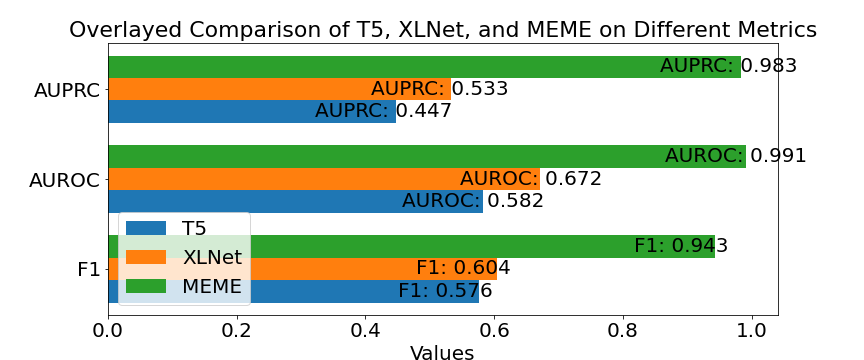
\includegraphics[width=\columnwidth]{figures/bar2.png}}
% \caption{Comparative Analysis of different encoder-only LLMs benchmarked against one another. Medbert (MEME) is optimized for medical tasks so the performance gap is evident.}
% \label{bar-22}
% \end{center}
% \vskip -0.2in
% \end{figure}

% Since we employed a frozen MedBert encoder in this work, we also \iffalse One intriguing aspect of our research involved evaluating \fi evaluated different Large Language Models (LLMs) to observe their performance variations in our analysis. \iffalse Since our model representations are generated by frozen LLM encoders, we \fi We investigated the effect of other encoder-only backbones (t5 and XLNet) on overall predictive performance. \iffalse operates by freezing the LLM encoders, the embeddings are determined solely by the millions to billions of parameters established during their pretraining in these extensive models. Initially, our project utilized the standard version of DistilBERT as the LLM, yielding satisfactory results. However, due to the critical importance of accuracy and precision in healthcare, we transitioned to a specialized BERT model trained on medical text, which appeared more suitable for our needs. \fi
% As shown in Figure \ref{bar-22}, MEME using a MedBert encoder displayed noticeably higher performance.

% \iffalse Therefore, we experimented with two other encoder-only based LLMs: XLNet and T5 (we extracted the encoder only of this encoder-decoder model), finding them more suited for text-classification tasks. We initially considered using more LLMs, such as decoder-only models like LLaMA-2-7b and phi2, for text classification tasks. However, recognizing that these are typically optimized for text generation, we determined that such a comparison might not provide a fair ``apples to apples'' assessment. We therefore provide the results in Figure \ref{bar-22} of the benchmark with the performance of other encoder-based models: \fi

% \iffalse This consideration underscores the dynamic nature of LLM research and the importance of continuously evaluating the suitability of different models for specific tasks, particularly in sensitive fields like healthcare. \fi

% \subsection{Generalization across datasets}

% % Show discrepancy with UCLA results - even when training on UCLA and testing on MIMIC, there is a substantial performance drop. [Maybe for discussion: even though mixed sample training would alleviate this, this highlights that there is still a gap in the generalizability of these models.]

% A recent critique of healthcare AI applications identified the lack of external validation and therefore potential overfitting to existing publicly available data. Indeed, we observed that while our approach and our reference models displayed strong within-dataset performance using a train-test split, performance was reduced when externally validated across institution (Figure \ref{bar13}.)

% \iffalse 
% One validation study we conducted on our Multimodal method involved attempting to validate our results at another hospital institution. While we observed exceptional performance when the method was validated within its own environment, testing it at a different institution provides a measure of our method's generalizability. To this end, we ran inference on our institutional dataset with our model trained on MIMIC and obtained rather interesting results.
% \fi

% \iffalse
% In summary, our method did not achieve similar performance levels when validated on this external institutional EHR. After thorough testing, we concluded that this discrepancy is likely not due to overfitting or model-related issues, but more likely due to the nature of the data itself. EHR data is not only widely heterogeneous but also varies significantly according to geographic regions. For instance, MIMIC is sourced from the Greater Boston area, which has a predominantly well-educated and Caucasian population, which may not be generalizable to the rest of the world. This hypothesis was further tested by training a model on our private institutional dataset. We found that while performance remained high when training and testing within the same EHR system, there was a noticeable performance drop in both validation experiments when the datasets were interchanged and validated on one another, as illustrated in Figure \ref{bar13}. This observation underscores the importance of considering geographic and institutional variations in EHR data while developing and validating healthcare models. It suggests that models highly effective in one setting may not necessarily perform equally well in another, due to the unique characteristics of healthcare data in different locales.
% \fi

% \iffalse
% Furthermore, while building a training dataset that combines MIMIC and our institutional EHR could alleviate this performance drop-off, it is important to highlight that there still exists a gap in generalizability for this model. \textbf{The publicly available MIMIC-IV ED dataset, in its current form, appears to be insufficient for ensuring generalization across diverse healthcare systems. }
% \fi % moving to discussion

% % \subsection{Concordant and Discordant Pairs Analysis}

% We performed a qualitative error analysis on the top 10 and bottom 10 scoring exemplars in our institutional dataset to gain insight into this performance gap. \textit{Concordant} cases were defined as those which the model scored highly and were correctly identified, or scored lowly and correctly not 
% \begin{figure}[h!]
% \vskip 0.2in
% \begin{center}
% \label{bar}
% \centerline{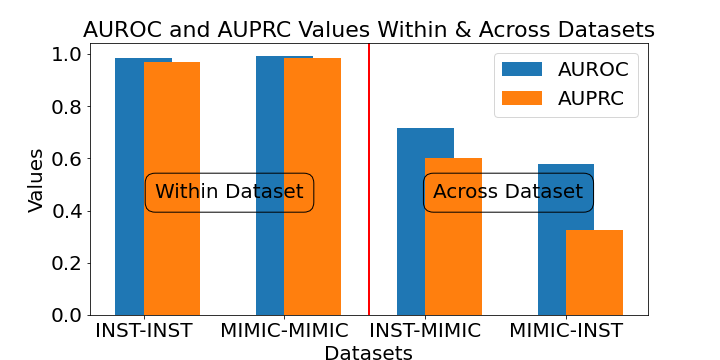
\includegraphics[width=\columnwidth]{figures/bar.png}}
% \caption{Comparative Analysis of AUROC and AUPRC Values for Intra- and Inter-Dataset Evaluations: This bar chart illustrates the AUROC and AUPRC values of different models, where the models themselves are represented by their training and testing datasets (e.g., MIMIC-MIMIC).}
% \label{bar13}
% \end{center}
% \vskip -0.2in
% \end{figure}
% flagged, and \textit{Discordant} cases were defined as vice versa. We found no systematic patterns or attributes of patients that explained this gap. However, the heterogeneity across EHR systems could be a reason behind this inconclusive finding and is worth further investigation.

% \iffalse 
% \subsubsection{Within Dataset}

% \textbf{Concordant Pairs:}Analysis revealed 134 cases where all models uniformly predicted patient disposition, typically in older patients with serious, unspecified conditions (e.g., ICD-10 code: [R410], disorientation, unspecified; ICD-10 code: [R4182], altered mental status, unspecified), lacking medication history (e.g., the pyxis modality was NaN), and typical chief complaints that would lead to hospital admission. Another 260 cases unanimously indicated no hospital admission, generally involving walk-ins with less severe issues (e.g. vertigo).

% \textbf{Discordant Pairs: }Identifying 203 discordant pairs was more complex. These cases showed a mismatch between single modality predictions and MEME's output (e.g., single modalities all predicted 0, while MEME predicted 1, and vice versa), with no apparent data-driven rationale. Notably, single modalities were confident in their predictions where MEME was not, and vice versa.

% \subsubsection{Across Dataset}

% \textbf{Concordant Pairs:} We next explored across the dataset, running the same analysis as before. When examining the results from the MIMIC-trained model validated on the insititutional data, we identified 784 out of 900k samples where all models categorized ``not admit to the hospital," and 0 instances where all models predicted an admission to the hospital. For this small cohort of 784, many of these patients again had manageable conditions and nothing out of the ordinary (e.g., chest pain).

% \textbf{Discordant Pairs:} We identified 4536 patients whose single modality models and multimodal models differed in their predictions. Interestingly, it always seemed one-sided in the discordant pairs, where all the single modality models predicted 0, and MEME predicted 1. There were instances where MEME predicted correctly, but also instances where it was incorrect. A closer look at the probabilities again showed that MEME was fairly confident in its predictions, leaving an unclear explanation to its decision making. However we should note these results may be affected by the heterogeneity of different EHR systems.

% In both within and across dataset analyses, concordant cases highlighted predictable patterns, while discordant ones revealed intriguing inconsistencies, particularly involving the MEME model's unique predictions. Further investigation might be needed to decode the underlying factors, especially for discordant pairs.

% \fi

% \section{Discussion}

% \subsection{Limitations}

% One crucial limitation of the model, is the lack of external validity. While building a training dataset that combines MIMIC and our institutional EHR, or performing external-site-specific fine tuning could alleviate this performance drop-off, it is important to highlight that there still exists a gap in generalizability for this model and competitors, as identified by Wornow and colleagues \cite{wornow_shaky_2023}. In addition to patient population differences, it is possible and likely that protocols around patient care vary across site and over time such that the same patient would experience different outcomes depending on when and where they experienced care. \textbf{Therefore we conclude that current models developed on the publicly available MIMIC-IV ED dataset appear to be insufficient for ensuring true generalization across diverse healthcare systems.}

% \iffalse interpretability in its decision-making processes. This issue is evident, as demonstrated by our generalization experiment, where the model's performance dropped when using a different dataset. \fi

% \iffalse 
% Furthermore, we observed variability in decision-making even within the same sample, as shown by the analysis of concordant and discordant pairs. Another pervasive challenge in this field is the ambiguity surrounding the type of knowledge embedded in pre-trained models. Although the MedBERT model card provides a summary of its pre-training process, the finer details of this process remain unknown. This pre-existing knowledge undeniably influences the model's behavior, further complicating the issue of interpretability. 
% \fi

% Another limitation of this work is our inability to release our private institutional data, due to privacy restrictions and institutional policy. This highlights the significance of independent benchmarks, and underscores the necessity of external validation, for example benchmark datasets and tasks such as MC-BEC \cite{chen2023multimodal}.

% \subsection{Future Works}

% \iffalse Some future work that our group is currently exploring includes various use cases for pseudo-notes, as this clinical text can be applied beyond mere classification tasks.\fi This approach can be extended beyond classification tasks. These applications encompass, but are not limited to, Retrieval Augmented Generation (RAG), recommendation systems, and other clinical tasks associated with textual modalities. Additionally, another promising direction could involve pre-training a Large Language Model from scratch, utilizing pseudo-notes sourced from multiple institutions. This approach aims to build a pre-trained model fundamentally based on structured Electronic Health Records, potentially enhancing its relevance and efficacy in healthcare contexts.

% \subsection{Conclusion}
% In this paper we introduced our model MEME, an approach for transforming multimodal tabular EHR data into clinical pseudo-notes. This transformation significantly enhances the interpretability of our data inputs and utility of EHR data in various healthcare-related tasks. The pseudo-notes method not only simplifies data handling but also effectively bridges the gap between traditional EHR formats and advanced NLP techniques employed in modern machine learning.

% A key finding from our study is the superior performance of the multimodal strategy employed by MEME. It outperforms a traditional ensembling machine learning method, single-modality and single-embedding methods, demonstrating the benefits of encoding different components of EHR separately. This approach allows for a more comprehensive representation of a patient's medical profile, capturing a broader spectrum of medical information crucial for accurate predictions. It's also worth noting that this approach can be extended to other clinical tasks that can be defined within the EHR. \iffalse , and can further be extended on all types of tasks. \fi

% However, our findings also highlight a significant challenge in the field of EHR analysis: the limited generalizability of models across different hospital institutions. Despite its strengths, the representation derived from the MIMIC-IV Database proved insufficient for generalization across diverse healthcare systems. This underscores the need for more representative publicly available datasets that can generalize to other EHR systems.

% % \subsection{Code \& Data}

% % Code will be made available on Github and MIMIC-IV ED data is available online.

% \subsection{Impact Statement}
% % positive - it offers an interface between modern AI (LLMs) and healthcare
% % negative - it does not directly address the potential biases in LLMs, and therefore could potentially introduce existing issues with LLMs into healthcare applications. More work is needed on this front before it's ready for prime time

% The goal of this work is to advance the field of Machine Learning in Healthcare, and thus presents a novel potential interface between modern NLP (LLMs) and clinical data. However, this work does not directly address issues involving performance and bias of all forms within LLMs and thus potentially introduces these issues into healthcare applications. This, coupled with our limited inter-site performance, highlight an urgent need for inter-site validation and further study before these models can leave the laboratory. 

% \iffalse This paper presents work whose goal is to advance the field of Machine Learning in Healthcare. While the approach seems to work well within an intra-hospital setting, we demonstrated in the paper that there is a need for more generalizable public datasets within the ML for healthcare community. In addition, MedBERT, used in our analysis, could be subject to potential bias in its pre-training scheme, influencing MEME's decision-making processes. Therefore, the MedBERT model can be replaced with more advanced backbones that are currently being developed in the LLM space extending its applicability as better representation models are created from these pre-trained models. \fi



% % \subsection{Code and Data}

% % Code will be public on github. MIMIC-IV ED can be found https://physionet.org/content/mimic-iv-ed/2.2/

% % \section{Electronic Submission}
% % \label{submission}

% % Submission to ICML 2024 will be entirely electronic, via a web site
% % (not email). Information about the submission process and \LaTeX\ templates
% % are available on the conference web site at:
% % \begin{center}
% % \textbf{\texttt{http://icml.cc/}}
% % \end{center}

% % The guidelines below will be enforced for initial submissions and
% % camera-ready copies. Here is a brief summary:
% % \begin{itemize}
% % \item Submissions must be in PDF\@. 
% % \item \textbf{New to this year}: If your paper has appendices, submit the appendix together with the main body and the references \textbf{as a single file}. Reviewers will not look for appendices as a separate PDF file. So if you submit such an extra file, reviewers will very likely miss it.
% % \item Page limit: The main body of the paper has to be fitted to 8 pages, excluding references and appendices; the space for the latter two is not limited. For the final version of the paper, authors can add one extra page to the main body.
% % \item \textbf{Do not include author information or acknowledgements} in your
% %     initial submission.
% % \item Your paper should be in \textbf{10 point Times font}.
% % \item Make sure your PDF file only uses Type-1 fonts.
% % \item Place figure captions \emph{under} the figure (and omit titles from inside
% %     the graphic file itself). Place table captions \emph{over} the table.
% % \item References must include page numbers whenever possible and be as complete
% %     as possible. Place multiple citations in chronological order.
% % \item Do not alter the style template; in particular, do not compress the paper
% %     format by reducing the vertical spaces.
% % \item Keep your abstract brief and self-contained, one paragraph and roughly
% %     4--6 sentences. Gross violations will require correction at the
% %     camera-ready phase. The title should have content words capitalized.
% % \end{itemize}

% % \subsection{Submitting Papers}

% % \textbf{Paper Deadline:} The deadline for paper submission that is
% % advertised on the conference website is strict. If your full,
% % anonymized, submission does not reach us on time, it will not be
% % considered for publication. 

% % \textbf{Anonymous Submission:} ICML uses double-blind review: no identifying
% % author information may appear on the title page or in the paper
% % itself. \cref{author info} gives further details.

% % \textbf{Simultaneous Submission:} ICML will not accept any paper which,
% % at the time of submission, is under review for another conference or
% % has already been published. This policy also applies to papers that
% % overlap substantially in technical content with conference papers
% % under review or previously published. ICML submissions must not be
% % submitted to other conferences and journals during ICML's review
% % period.
% % %Authors may submit to ICML substantially different versions of journal papers
% % %that are currently under review by the journal, but not yet accepted
% % %at the time of submission.
% % Informal publications, such as technical
% % reports or papers in workshop proceedings which do not appear in
% % print, do not fall under these restrictions.

% % \medskip

% % Authors must provide their manuscripts in \textbf{PDF} format.
% % Furthermore, please make sure that files contain only embedded Type-1 fonts
% % (e.g.,~using the program \texttt{pdffonts} in linux or using
% % File/DocumentProperties/Fonts in Acrobat). Other fonts (like Type-3)
% % might come from graphics files imported into the document.

% % Authors using \textbf{Word} must convert their document to PDF\@. Most
% % of the latest versions of Word have the facility to do this
% % automatically. Submissions will not be accepted in Word format or any
% % format other than PDF\@. Really. We're not joking. Don't send Word.

% % Those who use \textbf{\LaTeX} should avoid including Type-3 fonts.
% % Those using \texttt{latex} and \texttt{dvips} may need the following
% % two commands:

% % {\footnotesize
% % \begin{verbatim}
% % dvips -Ppdf -tletter -G0 -o paper.ps paper.dvi
% % ps2pdf paper.ps
% % \end{verbatim}}
% % It is a zero following the ``-G'', which tells dvips to use
% % the config.pdf file. Newer \TeX\ distributions don't always need this
% % option.

% % Using \texttt{pdflatex} rather than \texttt{latex}, often gives better
% % results. This program avoids the Type-3 font problem, and supports more
% % advanced features in the \texttt{microtype} package.

% % \textbf{Graphics files} should be a reasonable size, and included from
% % an appropriate format. Use vector formats (.eps/.pdf) for plots,
% % lossless bitmap formats (.png) for raster graphics with sharp lines, and
% % jpeg for photo-like images.

% % The style file uses the \texttt{hyperref} package to make clickable
% % links in documents. If this causes problems for you, add
% % \texttt{nohyperref} as one of the options to the \texttt{icml2024}
% % usepackage statement.


% % \subsection{Submitting Final Camera-Ready Copy}

% % The final versions of papers accepted for publication should follow the
% % same format and naming convention as initial submissions, except that
% % author information (names and affiliations) should be given. See
% % \cref{final author} for formatting instructions.

% % The footnote, ``Preliminary work. Under review by the International
% % Conference on Machine Learning (ICML). Do not distribute.'' must be
% % modified to ``\textit{Proceedings of the
% % $\mathit{41}^{st}$ International Conference on Machine Learning},
% % Vienna, Austria, PMLR 235, 2024.
% % Copyright 2024 by the author(s).''

% % For those using the \textbf{\LaTeX} style file, this change (and others) is
% % handled automatically by simply changing
% % $\mathtt{\backslash usepackage\{icml2024\}}$ to
% % $$\mathtt{\backslash usepackage[accepted]\{icml2024\}}$$
% % Authors using \textbf{Word} must edit the
% % footnote on the first page of the document themselves.

% % Camera-ready copies should have the title of the paper as running head
% % on each page except the first one. The running title consists of a
% % single line centered above a horizontal rule which is $1$~point thick.
% % The running head should be centered, bold and in $9$~point type. The
% % rule should be $10$~points above the main text. For those using the
% % \textbf{\LaTeX} style file, the original title is automatically set as running
% % head using the \texttt{fancyhdr} package which is included in the ICML
% % 2024 style file package. In case that the original title exceeds the
% % size restrictions, a shorter form can be supplied by using

% % \verb|\icmltitlerunning{...}|

% % just before $\mathtt{\backslash begin\{document\}}$.
% % Authors using \textbf{Word} must edit the header of the document themselves.

% % \section{Format of the Paper}

% % All submissions must follow the specified format.

% % \subsection{Dimensions}




% % The text of the paper should be formatted in two columns, with an
% % overall width of 6.75~inches, height of 9.0~inches, and 0.25~inches
% % between the columns. The left margin should be 0.75~inches and the top
% % margin 1.0~inch (2.54~cm). The right and bottom margins will depend on
% % whether you print on US letter or A4 paper, but all final versions
% % must be produced for US letter size.
% % Do not write anything on the margins.

% % The paper body should be set in 10~point type with a vertical spacing
% % of 11~points. Please use Times typeface throughout the text.

% % \subsection{Title}

% % The paper title should be set in 14~point bold type and centered
% % between two horizontal rules that are 1~point thick, with 1.0~inch
% % between the top rule and the top edge of the page. Capitalize the
% % first letter of content words and put the rest of the title in lower
% % case.

% % \subsection{Author Information for Submission}
% % \label{author info}

% % ICML uses double-blind review, so author information must not appear. If
% % you are using \LaTeX\/ and the \texttt{icml2024.sty} file, use
% % \verb+\icmlauthor{...}+ to specify authors and \verb+\icmlaffiliation{...}+ to specify affiliations. (Read the TeX code used to produce this document for an example usage.) The author information
% % will not be printed unless \texttt{accepted} is passed as an argument to the
% % style file.
% % Submissions that include the author information will not
% % be reviewed.

% % \subsubsection{Self-Citations}

% % If you are citing published papers for which you are an author, refer
% % to yourself in the third person. In particular, do not use phrases
% % that reveal your identity (e.g., ``in previous work \cite{langley00}, we
% % have shown \ldots'').

% % Do not anonymize citations in the reference section. The only exception are manuscripts that are
% % not yet published (e.g., under submission). If you choose to refer to
% % such unpublished manuscripts \cite{anonymous}, anonymized copies have
% % to be submitted
% % as Supplementary Material via OpenReview\@. However, keep in mind that an ICML
% % paper should be self contained and should contain sufficient detail
% % for the reviewers to evaluate the work. In particular, reviewers are
% % not required to look at the Supplementary Material when writing their
% % review (they are not required to look at more than the first $8$ pages of the submitted document).

% % \subsubsection{Camera-Ready Author Information}
% % \label{final author}

% % If a paper is accepted, a final camera-ready copy must be prepared.
% % %
% % For camera-ready papers, author information should start 0.3~inches below the
% % bottom rule surrounding the title. The authors' names should appear in 10~point
% % bold type, in a row, separated by white space, and centered. Author names should
% % not be broken across lines. Unbolded superscripted numbers, starting 1, should
% % be used to refer to affiliations.

% % Affiliations should be numbered in the order of appearance. A single footnote
% % block of text should be used to list all the affiliations. (Academic
% % affiliations should list Department, University, City, State/Region, Country.
% % Similarly for industrial affiliations.)

% % Each distinct affiliations should be listed once. If an author has multiple
% % affiliations, multiple superscripts should be placed after the name, separated
% % by thin spaces. If the authors would like to highlight equal contribution by
% % multiple first authors, those authors should have an asterisk placed after their
% % name in superscript, and the term ``\textsuperscript{*}Equal contribution"
% % should be placed in the footnote block ahead of the list of affiliations. A
% % list of corresponding authors and their emails (in the format Full Name
% % \textless{}email@domain.com\textgreater{}) can follow the list of affiliations.
% % Ideally only one or two names should be listed.

% % A sample file with author names is included in the ICML2024 style file
% % package. Turn on the \texttt{[accepted]} option to the stylefile to
% % see the names rendered. All of the guidelines above are implemented
% % by the \LaTeX\ style file.

% % \subsection{Abstract}

% % The paper abstract should begin in the left column, 0.4~inches below the final
% % address. The heading `Abstract' should be centered, bold, and in 11~point type.
% % The abstract body should use 10~point type, with a vertical spacing of
% % 11~points, and should be indented 0.25~inches more than normal on left-hand and
% % right-hand margins. Insert 0.4~inches of blank space after the body. Keep your
% % abstract brief and self-contained, limiting it to one paragraph and roughly 4--6
% % sentences. Gross violations will require correction at the camera-ready phase.

% % \subsection{Partitioning the Text}

% % You should organize your paper into sections and paragraphs to help
% % readers place a structure on the material and understand its
% % contributions.

% % \subsubsection{Sections and Subsections}

% % Section headings should be numbered, flush left, and set in 11~pt bold
% % type with the content words capitalized. Leave 0.25~inches of space
% % before the heading and 0.15~inches after the heading.

% % Similarly, subsection headings should be numbered, flush left, and set
% % in 10~pt bold type with the content words capitalized. Leave
% % 0.2~inches of space before the heading and 0.13~inches afterward.

% % Finally, subsubsection headings should be numbered, flush left, and
% % set in 10~pt small caps with the content words capitalized. Leave
% % 0.18~inches of space before the heading and 0.1~inches after the
% % heading.

% % Please use no more than three levels of headings.

% % \subsubsection{Paragraphs and Footnotes}

% % Within each section or subsection, you should further partition the
% % paper into paragraphs. Do not indent the first line of a given
% % paragraph, but insert a blank line between succeeding ones.

% % You can use footnotes\footnote{Footnotes
% % should be complete sentences.} to provide readers with additional
% % information about a topic without interrupting the flow of the paper.
% % Indicate footnotes with a number in the text where the point is most
% % relevant. Place the footnote in 9~point type at the bottom of the
% % column in which it appears. Precede the first footnote in a column
% % with a horizontal rule of 0.8~inches.\footnote{Multiple footnotes can
% % appear in each column, in the same order as they appear in the text,
% % but spread them across columns and pages if possible.}

% % \begin{figure}[ht]
% % \vskip 0.2in
% % \begin{center}
% % \centerline{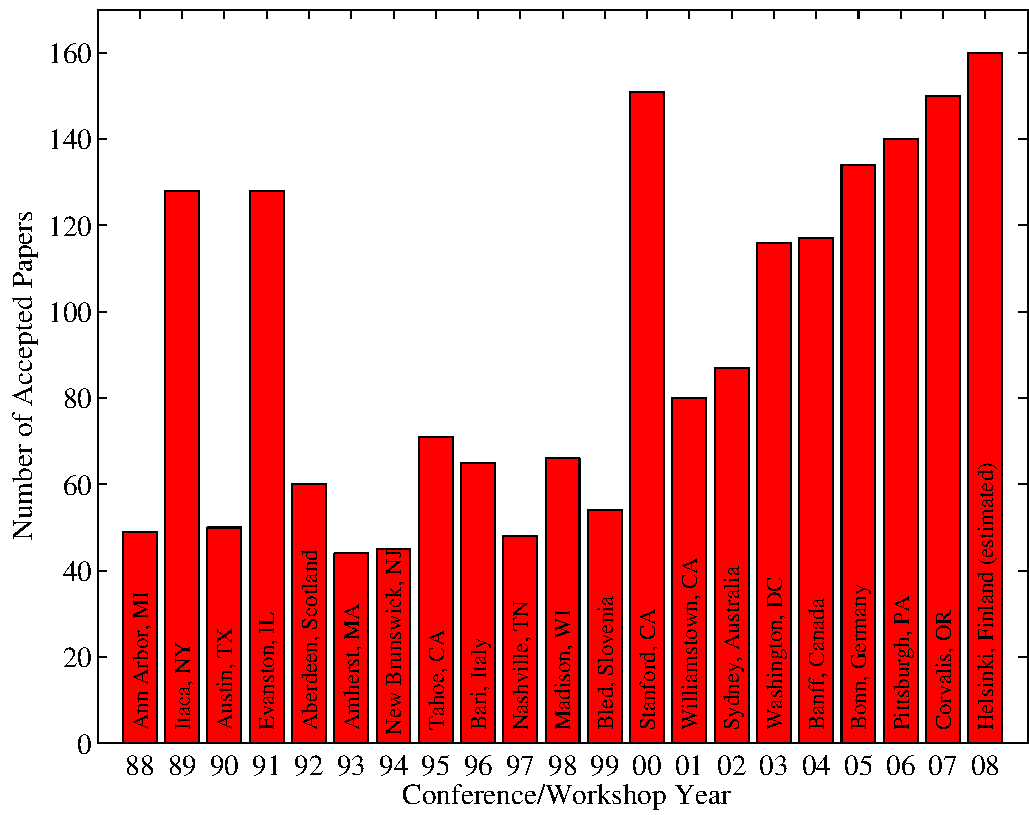
\includegraphics[width=\columnwidth]{icml_numpapers}}
% % \caption{Historical locations and number of accepted papers for International
% % Machine Learning Conferences (ICML 1993 -- ICML 2008) and International
% % Workshops on Machine Learning (ML 1988 -- ML 1992). At the time this figure was
% % produced, the number of accepted papers for ICML 2008 was unknown and instead
% % estimated.}
% % \label{icml-historical}
% % \end{center}
% % \vskip -0.2in
% % \end{figure}

% % \subsection{Figures}

% % You may want to include figures in the paper to illustrate
% % your approach and results. Such artwork should be centered,
% % legible, and separated from the text. Lines should be dark and at
% % least 0.5~points thick for purposes of reproduction, and text should
% % not appear on a gray background.

% % Label all distinct components of each figure. If the figure takes the
% % form of a graph, then give a name for each axis and include a legend
% % that briefly describes each curve. Do not include a title inside the
% % figure; instead, the caption should serve this function.

% % Number figures sequentially, placing the figure number and caption
% % \emph{after} the graphics, with at least 0.1~inches of space before
% % the caption and 0.1~inches after it, as in
% % \cref{icml-historical}. The figure caption should be set in
% % 9~point type and centered unless it runs two or more lines, in which
% % case it should be flush left. You may float figures to the top or
% % bottom of a column, and you may set wide figures across both columns
% % (use the environment \texttt{figure*} in \LaTeX). Always place
% % two-column figures at the top or bottom of the page.

% % \subsection{Algorithms}

% % If you are using \LaTeX, please use the ``algorithm'' and ``algorithmic''
% % environments to format pseudocode. These require
% % the corresponding stylefiles, algorithm.sty and
% % algorithmic.sty, which are supplied with this package.
% % \cref{alg:example} shows an example.

% % \begin{algorithm}[tb]
% %    \caption{Bubble Sort}
% %    \label{alg:example}
% % \begin{algorithmic}
% %    \STATE {\bfseries Input:} data $x_i$, size $m$
% %    \REPEAT
% %    \STATE Initialize $noChange = true$.
% %    \FOR{$i=1$ {\bfseries to} $m-1$}
% %    \IF{$x_i > x_{i+1}$}
% %    \STATE Swap $x_i$ and $x_{i+1}$
% %    \STATE $noChange = false$
% %    \ENDIF
% %    \ENDFOR
% %    \UNTIL{$noChange$ is $true$}
% % \end{algorithmic}
% % \end{algorithm}

% % \subsection{Tables}

% % You may also want to include tables that summarize material. Like
% % figures, these should be centered, legible, and numbered consecutively.
% % However, place the title \emph{above} the table with at least
% % 0.1~inches of space before the title and the same after it, as in
% % \cref{sample-table}. The table title should be set in 9~point
% % type and centered unless it runs two or more lines, in which case it
% % should be flush left.

% % % Note use of \abovespace and \belowspace to get reasonable spacing
% % % above and below tabular lines.

% % \begin{table}[t]
% % \caption{Classification accuracies for naive Bayes and flexible
% % Bayes on various data sets.}
% % \label{sample-table}
% % \vskip 0.15in
% % \begin{center}
% % \begin{small}
% % \begin{sc}
% % \begin{tabular}{lcccr}
% % \toprule
% % Data set & Naive & Flexible & Better? \\
% % \midrule
% % Breast    & 95.9$\pm$ 0.2& 96.7$\pm$ 0.2& $\surd$ \\
% % Cleveland & 83.3$\pm$ 0.6& 80.0$\pm$ 0.6& $\times$\\
% % Glass2    & 61.9$\pm$ 1.4& 83.8$\pm$ 0.7& $\surd$ \\
% % Credit    & 74.8$\pm$ 0.5& 78.3$\pm$ 0.6&         \\
% % Horse     & 73.3$\pm$ 0.9& 69.7$\pm$ 1.0& $\times$\\
% % Meta      & 67.1$\pm$ 0.6& 76.5$\pm$ 0.5& $\surd$ \\
% % Pima      & 75.1$\pm$ 0.6& 73.9$\pm$ 0.5&         \\
% % Vehicle   & 44.9$\pm$ 0.6& 61.5$\pm$ 0.4& $\surd$ \\
% % \bottomrule
% % \end{tabular}
% % \end{sc}
% % \end{small}
% % \end{center}
% % \vskip -0.1in
% % \end{table}

% % Tables contain textual material, whereas figures contain graphical material.
% % Specify the contents of each row and column in the table's topmost
% % row. Again, you may float tables to a column's top or bottom, and set
% % wide tables across both columns. Place two-column tables at the
% % top or bottom of the page.

% % \subsection{Theorems and such}
% % The preferred way is to number definitions, propositions, lemmas, etc. consecutively, within sections, as shown below.
% % \begin{definition}
% % \label{def:inj}
% % A function $f:X \to Y$ is injective if for any $x,y\in X$ different, $f(x)\ne f(y)$.
% % \end{definition}
% % Using \cref{def:inj} we immediate get the following result:
% % \begin{proposition}
% % If $f$ is injective mapping a set $X$ to another set $Y$, 
% % the cardinality of $Y$ is at least as large as that of $X$
% % \end{proposition}
% % \begin{proof} 
% % Left as an exercise to the reader. 
% % \end{proof}
% % \cref{lem:usefullemma} stated next will prove to be useful.
% % \begin{lemma}
% % \label{lem:usefullemma}
% % For any $f:X \to Y$ and $g:Y\to Z$ injective functions, $f \circ g$ is injective.
% % \end{lemma}
% % \begin{theorem}
% % \label{thm:bigtheorem}
% % If $f:X\to Y$ is bijective, the cardinality of $X$ and $Y$ are the same.
% % \end{theorem}
% % An easy corollary of \cref{thm:bigtheorem} is the following:
% % \begin{corollary}
% % If $f:X\to Y$ is bijective, 
% % the cardinality of $X$ is at least as large as that of $Y$.
% % \end{corollary}
% % \begin{assumption}
% % The set $X$ is finite.
% % \label{ass:xfinite}
% % \end{assumption}
% % \begin{remark}
% % According to some, it is only the finite case (cf. \cref{ass:xfinite}) that is interesting.
% % \end{remark}
% % %restatable

% % \subsection{Citations and References}

% % Please use APA reference format regardless of your formatter
% % or word processor. If you rely on the \LaTeX\/ bibliographic
% % facility, use \texttt{natbib.sty} and \texttt{icml2024.bst}
% % included in the style-file package to obtain this format.

% % Citations within the text should include the authors' last names and
% % year. If the authors' names are included in the sentence, place only
% % the year in parentheses, for example when referencing Arthur Samuel's
% % pioneering work \yrcite{Samuel59}. Otherwise place the entire
% % reference in parentheses with the authors and year separated by a
% % comma \cite{Samuel59}. List multiple references separated by
% % semicolons \cite{kearns89,Samuel59,mitchell80}. Use the `et~al.'
% % construct only for citations with three or more authors or after
% % listing all authors to a publication in an earlier reference \cite{MachineLearningI}.

% % Authors should cite their own work in the third person
% % in the initial version of their paper submitted for blind review.
% % Please refer to \cref{author info} for detailed instructions on how to
% % cite your own papers.

% % Use an unnumbered first-level section heading for the references, and use a
% % hanging indent style, with the first line of the reference flush against the
% % left margin and subsequent lines indented by 10 points. The references at the
% % end of this document give examples for journal articles \cite{Samuel59},
% % conference publications \cite{langley00}, book chapters \cite{Newell81}, books
% % \cite{DudaHart2nd}, edited volumes \cite{MachineLearningI}, technical reports
% % \cite{mitchell80}, and dissertations \cite{kearns89}.

% % Alphabetize references by the surnames of the first authors, with
% % single author entries preceding multiple author entries. Order
% % references for the same authors by year of publication, with the
% % earliest first. Make sure that each reference includes all relevant
% % information (e.g., page numbers).

% % Please put some effort into making references complete, presentable, and
% % consistent, e.g. use the actual current name of authors.
% % If using bibtex, please protect capital letters of names and
% % abbreviations in titles, for example, use \{B\}ayesian or \{L\}ipschitz
% % in your .bib file.

% % \section*{Accessibility}
% % Authors are kindly asked to make their submissions as accessible as possible for everyone including people with disabilities and sensory or neurological differences.
% % Tips of how to achieve this and what to pay attention to will be provided on the conference website \url{http://icml.cc/}.

% % \section*{Software and Data}

% % If a paper is accepted, we strongly encourage the publication of software and data with the
% % camera-ready version of the paper whenever appropriate. This can be
% % done by including a URL in the camera-ready copy. However, \textbf{do not}
% % include URLs that reveal your institution or identity in your
% % submission for review. Instead, provide an anonymous URL or upload
% % the material as ``Supplementary Material'' into the OpenReview reviewing
% % system. Note that reviewers are not required to look at this material
% % when writing their review.

% % % Acknowledgements should only appear in the accepted version.
% % \section*{Acknowledgements}

% % \textbf{Do not} include acknowledgements in the initial version of
% % the paper submitted for blind review.

% % If a paper is accepted, the final camera-ready version can (and
% % probably should) include acknowledgements. In this case, please
% % place such acknowledgements in an unnumbered section at the
% % end of the paper. Typically, this will include thanks to reviewers
% % who gave useful comments, to colleagues who contributed to the ideas,
% % and to funding agencies and corporate sponsors that provided financial
% % support.


% % % In the unusual situation where you want a paper to appear in the
% % % references without citing it in the main text, use \nocite
% % \nocite{langley00}
% \bibliography{example_paper}
% \bibliographystyle{icml2024}


% %%%%%%%%%%%%%%%%%%%%%%%%%%%%%%%%%%%%%%%%%%%%%%%%%%%%%%%%%%%%%%%%%%%%%%%%%%%%%%%
% %%%%%%%%%%%%%%%%%%%%%%%%%%%%%%%%%%%%%%%%%%%%%%%%%%%%%%%%%%%%%%%%%%%%%%%%%%%%%%%
% % APPENDIX
% %%%%%%%%%%%%%%%%%%%%%%%%%%%%%%%%%%%%%%%%%%%%%%%%%%%%%%%%%%%%%%%%%%%%%%%%%%%%%%%
% %%%%%%%%%%%%%%%%%%%%%%%%%%%%%%%%%%%%%%%%%%%%%%%%%%%%%%%%%%%%%%%%%%%%%%%%%%%%%%%
% \newpage
% \appendix
% \onecolumn
% \section{Appendix}
% \label{Appendix}
% \subsection{Example Pseudonotes}

% In Section \ref{pseudo}, we referred to the appendix to provide a verbose exploration of our pseudo-notes generation process, offering more detailed and illustrative examples. Building upon the foundation laid out earlier, we utilize color coordination to clearly delineate the  distinctions between information sourced directly from our raw EHR data and content that was dynamically generated through our script.

% \begin{multicols}{2}

% \textit{Arrival Information}\\
% \fbox{\begin{minipage}{15em}
% Patient \textcolor{red}{10000032}, a \textcolor{red}{52} year old \textcolor{red}{white female}, arrived via \textcolor{red}{ambulance} at \textcolor{red}{2180-05-06 19:17:00}. The patient's marital status is \textcolor{red}{widowed}. The patient's insurance is \textcolor{red}{other}. The patient's language is \textcolor{red}{english}.
% \end{minipage}}\\

% \textit{Emergency Department Disposition}\\
% \fbox{\begin{minipage}{15em}
% The ED disposition was \textcolor{red}{admitted} at \textcolor{red}{2180-05-06 23:30:00}. The patient died on \textcolor{red}{2180-09-09}.
% \end{minipage}}\\

% \textit{Triage}\\
% \fbox{\begin{minipage}{15em}
% At triage: temperature was \textcolor{red}{98.4}, pulse was \textcolor{red}{70}, respirations was \textcolor{red}{16}, o2 saturation was \textcolor{red}{97}, systolic blood pressure was \textcolor{red}{106}, diastolic blood pressure was \textcolor{red}{63}, pain was \textcolor{red}{0}, chief complaint was \textcolor{red}{abd pain}, \textcolor{red}{abdominal distention}. Acuity score was \textcolor{red}{3}.
% \end{minipage}}\\

% \textit{Medrecon}\\ 
% \fbox{\begin{minipage}{15em}
% The patient was previously taking the following medications: \textcolor{red}{albuterol sulfate}, \textcolor{red}{asthma/copd therapy - beta 2-adrenergic agents}, \textcolor{red}{inhaled}, \textcolor{red}{short acting}. \textcolor{red}{peg 3350-electrolytes}, \textcolor{red}{laxative - saline/osmotic mixtures}. \textcolor{red}{nicotine}, \textcolor{red}{smoking deterrents - nicotine-type}. \textcolor{red}{spironolactone [aldactone]}, \textcolor{red}{aldosterone receptor antagonists}. \textcolor{red}{emtricitabine-tenofovir [truvada]}, \textcolor{red}{antiretroviral - nucleoside and nucleotide analog rtis combinations}. \textcolor{red}{raltegravir [isentress]}, \textcolor{red}{antiretroviral - hiv-1 integrase strand transfer inhibitors}. \textcolor{red}{spironolactone [aldactone]}, \textcolor{red}{diuretic - aldosterone receptor antagonist}, \textcolor{red}{non-selective}. \textcolor{red}{furosemide, diuretic - loop}. \textcolor{red}{ipratropium bromide [atrovent hfa]}, \textcolor{red}{asthma/copd - anticholinergic agents}, \textcolor{red}{inhaled short acting}. \textcolor{red}{ergocalciferol (vitamin d2)}, \textcolor{red}{vitamins - d derivatives}.
% \end{minipage}} 

% \textit{Patient Vitals}\\
% \fbox{\begin{minipage}{15em}
% The patient had the following vitals: At \textcolor{red}{2180-05-06 23:04:00}, temperature was \textcolor{red}{97.7}, pulse was \textcolor{red}{79}, respirations was \textcolor{red}{16}, o2 saturation was \textcolor{red}{98}, systolic blood pressure was \textcolor{red}{107}, diastolic blood pressure was \textcolor{red}{60}, pain was \textcolor{red}{0}.
% \end{minipage}} \\

% \textit{Pyxis}\\
% \fbox{\begin{minipage}{15em}
% The patient received the following medications: At \textcolor{red}{2180-08-05 22:29:00}, \textcolor{red}{morphine} were administered. At \textcolor{red}{2180-08-05 22:55:00}, \textcolor{red}{donnatol (elixir), aluminum-magnesium hydrox.-simet, aluminum-magnesium hydrox.-simet, ondansetron, ondansetron} were administered. 
% \end{minipage}}\\

% \textit{Diagnostic Codes}\\
% \fbox{\begin{minipage}{15em}
% The patient received the following diagnostic codes: ICD-9 code: \textcolor{red}{[78959], other ascites}. ICD-9 code: \textcolor{red}{[07070], unspecified viral hepatitis c without hepatic coma}. ICD-9 code: \textcolor{red}{[5715], cirrhosis of liver nos}. ICD-9 code: \textcolor{red}{[v08], asymptomatic hiv infection}. 
% \end{minipage}}


% \end{multicols}

% \subsection{Model Descriptions}
% In the subsequent section, we delve into the \iffalse intricate \fi details of the model architectures employed by other single modality approaches and \iffalse proficient \fi machine learning methods. \iffalse , offering a comprehensive exploration for pedagogical clarity. \fi We disclose more detailed hyperparameters and architectural designs that constitute these models, facilitating a transparent benchmarking process. If there are any further questions after reading this section, feel free to contact the authors for more details.

% \textbf{Single Modality Specific  Methods}\\
% In our analysis, we presented six distinct model variations, each tailored to one of the six modalities used for predicting the target variable. While these models share similarities with our multimodal approach, they diverge in certain aspects as deliberate feature removal sets them apart from our multimodal methodology. These single modality approaches adhere to a more conventional Language Model (LLM) fine-tuning paradigm. However they still do slightly diverge from these approaches as well. In these single modality models, we froze each LLM encoder and trained a linear classifier to be able to learn the proper underlying representations to make a proper prediction.

% Moreover, unlike our multimodal model, these single modality models forego our second step to the network, which incorporates an additional self-attention layer step, as they do not necessitate learning a unified input. This \iffalse streamlined \fi approach reflects the task-specific focus of these models, optimizing for individual modality predictions without the need for a unified multimodal analysis.

% In terms of preprocessing, we used the same preprocessing steps as our multimodal approach and extracted the modality-specific subset Dataset object from the Hugging Face library for our analysis. Subsequently, we loaded these dataset objects into conventional PyTorch dataloaders for training the classifier. Similar to our multimodal approach, we also utilized the Cross-Entropy Loss and AdamW optimizer, with a learning rate of $5e-5$, and trained until the validation error converges. Additionally, we implemented a linear learning rate scheduler to adjust the model’s learning rate during training, thus tuning this hyperparameter, which impacts our overall model performance. We tracked F1 scores to assess the performance of our model after every epoch.

% \textbf{Multimodal Single Embedding Model}\\
% In our benchmarking study, we also included a model referred to as the Multimodal Single Embedding Model (MSEM). This inclusion represents the canonical LLM approach of \iffalse aimed to preemptively address potential queries about \fi consolidating all text data into a single embedding. The MSEM closely resembles single modality models in terms of architecture; however, it diverges primarily in its preprocessing step, where all text is merged into a single column and truncated during tokenization.

% The feasibility of an MSEM is largely constrained by context-length limitations imposed by BERT and other Large Language Models (LLMs). In our study, we focused on Emergency department EHR data, which encompassed six corresponding modalities. However, in broader applications like general EHR, the data can span as many as 10-20 different modalities related to a patient's health history. These limitations are significant as they potentially restrict the depth and breadth of data that can be effectively processed and analyzed by models like the MSEM.

% \textbf{Random Forest Classifier}\\
% Lastly, our benchmarking also involved training and fitting a Random Forest classifier. \iffalse Renowned as an ensemble learning technique, Random Forest is part of the decision tree-based algorithm family. Its strength lies in constructing multiple decision trees whose collective outputs are aggregated to yield predictions that are both robust and accurate. \fi We selected 1000 estimators, equivalent to creating 1000 trees. \iffalse Given our ample resources, handling this substantial number of estimators was feasible, thus influencing our choice of this particular hyperparameter. \fi 
% In contrast to our approach with pseudo-notes, the data preparation for the Random Forest classifier was markedly different. While BERT and transformer-based models primarily process text data, such an approach was not viable with the Random Forest. Consequently, we utilized the EHR data in its unaltered tabular format. To maintain consistency across our analyses, we filtered this data using the same patient subsets identified in the test, validation, and training sets of our transformer-based methods. Furthermore, we implemented one-hot encoding on various modalities, including medication reconciliation, ICD codes, and Pyxis drugs, to effectively prepare the data for the Random Forest model.

% %%%%%%%%%%%%%%%%%%%%%%%%%%%%%%%%%%%%%%%%%%%%%%%%%%%%%%%%%%%%%%%%%%%%%%%%%%%%%%%
% %%%%%%%%%%%%%%%%%%%%%%%%%%%%%%%%%%%%%%%%%%%%%%%%%%%%%%%%%%%%%%%%%%%%%%%%%%%%%%%
% \newpage
% % \subsection{Institutional Results \& Across datasets results}

% % \begin{table*}[h!]
% % \caption{The benchmarking metrics displayed for predicting ED disposition on our Institutional Dataset. Like the MIMIC results in our main paper, 95\% percent confidence intervals were calculated and displayed, along with Area under the receiver operator curve (AUROC), Area under the precision-recall curve (AUPRC) and F1 scores (with optimal thresholding) for our binary classification task.}
% % \vskip 0.15in
% % \begin{center}
% % \label{evaluation}
% % \begin{small}
% % \begin{sc}
% % \begin{tabular}{p{1.8cm}p{2.4cm}|ccc}
% % \toprule
% % & & & Institutional & \\  
% % Task & Method & F1 & AUROC & AUPRC \\
% % \hline

% % \multirow{6}{*}{Disposition}     & arrival   & 0.404 $\pm$ 0.003       & 0.514 $\pm$ 0.004         & 0.282 $\pm$ 0.004         \\
% %  & codes     & 0.671 $\pm$ 0.004       & 0.869 $\pm$ 0.002         & 0.667 $\pm$ 0.006         \\
% %  & pyxis     & 0.635 $\pm$ 0.004       & 0.844 $\pm$ 0.003         & 0.600 $\pm$ 0.006         \\
% %  & triage    & 0.445 $\pm$ 0.003       & 0.637 $\pm$ 0.003         & 0.328 $\pm$ 0.004         \\
% %  & vitals    & 0.620 $\pm$ 0.004       & 0.815 $\pm$ 0.003         & 0.534 $\pm$ 0.006         \\
% %  & MEME      & \textbf{0.915 $\pm$ 0.002} & \textbf{0.985 $\pm$ 0.001} & \textbf{0.970 $\pm$ 0.002} \\ \hline

% % \hline

% % \multirow{6}{*}{Discharge} & arrival & 0.553 $\pm$ 0.005       & 0.527 $\pm$ 0.007         & 0.401 $\pm$ 0.008         \\
% % & codes   & 0.554 $\pm$ 0.005       & 0.544 $\pm$ 0.006         & 0.412 $\pm$ 0.008         \\
% % & pyxis   & 0.555 $\pm$ 0.006       & 0.540 $\pm$ 0.006         & 0.408 $\pm$ 0.008         \\
% % & triage  & 0.553 $\pm$ 0.005       & 0.520 $\pm$ 0.006         & 0.396 $\pm$ 0.008         \\
% % & vitals  & 0.553 $\pm$ 0.006       & 0.529 $\pm$ 0.007         & 0.397 $\pm$ 0.008         \\
% % & MEME    & \textbf{0.568 $\pm$ 0.006} & \textbf{0.660 $\pm$ 0.006} & \textbf{0.553 $\pm$ 0.009} \\ \hline

% % \hline

% % \multirow{6}{*}{Mortality} & arrival & 0.061 $\pm$ 0.003       & 0.511 $\pm$ 0.018         & 0.032 $\pm$ 0.004         \\
% % & codes   & 0.079 $\pm$ 0.009       & 0.584 $\pm$ 0.017         & 0.041 $\pm$ 0.004         \\
% % & pyxis   & 0.060 $\pm$ 0.003       & 0.498 $\pm$ 0.018         & 0.032 $\pm$ 0.004         \\
% % & triage  & 0.060 $\pm$ 0.004       & 0.484 $\pm$ 0.017         & 0.029 $\pm$ 0.003         \\
% % & vitals  & \textbf{0.140 $\pm$ 0.027 }      & 0.570 $\pm$ 0.018         & \textbf{0.091 $\pm$ 0.018}         \\
% % & MEME    & 0.125 $\pm$ 0.013       & \textbf{0.646 $\pm$ 0.019}         & 0.067 $\pm$ 0.008         \\ \hline

% % \hline
% % \multirow{6}{*}{ICU} & arrival & 0.275 $\pm$ 0.006       & 0.518 $\pm$ 0.008         & 0.167 $\pm$ 0.006         \\
% %  & codes   & 0.298 $\pm$ 0.007       & 0.596 $\pm$ 0.008         & 0.208 $\pm$ 0.008         \\
% %  & pyxis   & 0.276 $\pm$ 0.006       & 0.529 $\pm$ 0.008         & 0.173 $\pm$ 0.006         \\
% %  & triage  & 0.276 $\pm$ 0.007       & 0.547 $\pm$ 0.008         & 0.180 $\pm$ 0.006         \\
% %  & vitals  & 0.275 $\pm$ 0.006       & 0.509 $\pm$ 0.008         & 0.161 $\pm$ 0.006         \\
% %  & MEME    & \textbf{0.346 $\pm$ 0.010}       & \textbf{0.658 $\pm$ 0.008}         & \textbf{0.269 $\pm$ 0.010 }        \\ 



% % \bottomrule
% % \end{tabular}
% % \end{sc}
% % \end{small}
% % \end{center}
% % \vskip -0.1in
% % \end{table*}

% % \begin{table*}[h!]
% % \caption{Results from our model trained on the MIMIC dataset and validated using our institutional database.}
% % \vskip 0.15in
% % \begin{center}
% % \label{evaluation}
% % \begin{small}
% % \begin{sc}
% % \begin{tabular}{p{1.8cm}p{2.4cm}|ccc}
% % \toprule
% % & & & MIMIC-Institutional & \\  
% % Task & Method & F1 & AUROC & AUPRC \\
% % \hline

% % \multirow{6}{*}{Disposition}     & arrival   & 0.404 $\pm$ 0.003       & 0.514 $\pm$ 0.004         & 0.282 $\pm$ 0.004         \\
% %  & codes     & 0.671 $\pm$ 0.004       & 0.869 $\pm$ 0.002         & 0.667 $\pm$ 0.006         \\
% %  & pyxis     & 0.635 $\pm$ 0.004       & 0.844 $\pm$ 0.003         & 0.600 $\pm$ 0.006         \\
% %  & triage    & 0.445 $\pm$ 0.003       & 0.637 $\pm$ 0.003         & 0.328 $\pm$ 0.004         \\
% %  & vitals    & 0.620 $\pm$ 0.004       & 0.815 $\pm$ 0.003         & 0.534 $\pm$ 0.006         \\
% %  & MEME      & \textbf{0.915 $\pm$ 0.002} & \textbf{0.985 $\pm$ 0.001} & \textbf{0.970 $\pm$ 0.002} \\ \hline

% % \hline

% % \multirow{6}{*}{Discharge} & arrival & 0.553 $\pm$ 0.005       & 0.527 $\pm$ 0.007         & 0.401 $\pm$ 0.008         \\
% % & codes   & 0.554 $\pm$ 0.005       & 0.544 $\pm$ 0.006         & 0.412 $\pm$ 0.008         \\
% % & pyxis   & 0.555 $\pm$ 0.006       & 0.540 $\pm$ 0.006         & 0.408 $\pm$ 0.008         \\
% % & triage  & 0.553 $\pm$ 0.005       & 0.520 $\pm$ 0.006         & 0.396 $\pm$ 0.008         \\
% % & vitals  & 0.553 $\pm$ 0.006       & 0.529 $\pm$ 0.007         & 0.397 $\pm$ 0.008         \\
% % & MEME    & \textbf{0.568 $\pm$ 0.006} & \textbf{0.660 $\pm$ 0.006} & \textbf{0.553 $\pm$ 0.009} \\ \hline

% % \hline

% % \multirow{6}{*}{Mortality} & arrival & 0.061 $\pm$ 0.003       & 0.511 $\pm$ 0.018         & 0.032 $\pm$ 0.004         \\
% % & codes   & 0.079 $\pm$ 0.009       & 0.584 $\pm$ 0.017         & 0.041 $\pm$ 0.004         \\
% % & pyxis   & 0.060 $\pm$ 0.003       & 0.498 $\pm$ 0.018         & 0.032 $\pm$ 0.004         \\
% % & triage  & 0.060 $\pm$ 0.004       & 0.484 $\pm$ 0.017         & 0.029 $\pm$ 0.003         \\
% % & vitals  & \textbf{0.140 $\pm$ 0.027 }      & 0.570 $\pm$ 0.018         & \textbf{0.091 $\pm$ 0.018}         \\
% % & MEME    & 0.125 $\pm$ 0.013       & \textbf{0.646 $\pm$ 0.019}         & 0.067 $\pm$ 0.008         \\ \hline

% % \hline
% % \multirow{6}{*}{ICU} & arrival & 0.275 $\pm$ 0.006       & 0.518 $\pm$ 0.008         & 0.167 $\pm$ 0.006         \\
% %  & codes   & 0.298 $\pm$ 0.007       & 0.596 $\pm$ 0.008         & 0.208 $\pm$ 0.008         \\
% %  & pyxis   & 0.276 $\pm$ 0.006       & 0.529 $\pm$ 0.008         & 0.173 $\pm$ 0.006         \\
% %  & triage  & 0.276 $\pm$ 0.007       & 0.547 $\pm$ 0.008         & 0.180 $\pm$ 0.006         \\
% %  & vitals  & 0.275 $\pm$ 0.006       & 0.509 $\pm$ 0.008         & 0.161 $\pm$ 0.006         \\
% %  & MEME    & \textbf{0.346 $\pm$ 0.010}       & \textbf{0.658 $\pm$ 0.008}         & \textbf{0.269 $\pm$ 0.010 }        \\ 



% % \bottomrule
% % \end{tabular}
% % \end{sc}
% % \end{small}
% % \end{center}
% % \vskip -0.1in
% % \end{table*}

% % \begin{table*}[h!]
% % \caption{Results from our model trained on our Institutional dataset and validated using the MIMIC database.}
% % \vskip 0.15in
% % \begin{center}
% % \label{evaluation}
% % \begin{small}
% % \begin{sc}
% % \begin{tabular}{p{1.8cm}p{2.4cm}|ccc}
% % \toprule
% % & & & Institutional-MIMIC & \\  
% % Task & Method & F1 & AUROC & AUPRC \\
% % \hline

% % \multirow{6}{*}{Disposition}     & arrival   & 0.404 $\pm$ 0.003       & 0.514 $\pm$ 0.004         & 0.282 $\pm$ 0.004         \\
% %  & codes     & 0.671 $\pm$ 0.004       & 0.869 $\pm$ 0.002         & 0.667 $\pm$ 0.006         \\
% %  & pyxis     & 0.635 $\pm$ 0.004       & 0.844 $\pm$ 0.003         & 0.600 $\pm$ 0.006         \\
% %  & triage    & 0.445 $\pm$ 0.003       & 0.637 $\pm$ 0.003         & 0.328 $\pm$ 0.004         \\
% %  & vitals    & 0.620 $\pm$ 0.004       & 0.815 $\pm$ 0.003         & 0.534 $\pm$ 0.006         \\
% %  & MEME      & \textbf{0.915 $\pm$ 0.002} & \textbf{0.985 $\pm$ 0.001} & \textbf{0.970 $\pm$ 0.002} \\ \hline

% % \hline

% % \multirow{6}{*}{Discharge} & arrival & 0.553 $\pm$ 0.005       & 0.527 $\pm$ 0.007         & 0.401 $\pm$ 0.008         \\
% % & codes   & 0.554 $\pm$ 0.005       & 0.544 $\pm$ 0.006         & 0.412 $\pm$ 0.008         \\
% % & pyxis   & 0.555 $\pm$ 0.006       & 0.540 $\pm$ 0.006         & 0.408 $\pm$ 0.008         \\
% % & triage  & 0.553 $\pm$ 0.005       & 0.520 $\pm$ 0.006         & 0.396 $\pm$ 0.008         \\
% % & vitals  & 0.553 $\pm$ 0.006       & 0.529 $\pm$ 0.007         & 0.397 $\pm$ 0.008         \\
% % & MEME    & \textbf{0.568 $\pm$ 0.006} & \textbf{0.660 $\pm$ 0.006} & \textbf{0.553 $\pm$ 0.009} \\ \hline

% % \hline

% % \multirow{6}{*}{Mortality} & arrival & 0.061 $\pm$ 0.003       & 0.511 $\pm$ 0.018         & 0.032 $\pm$ 0.004         \\
% % & codes   & 0.079 $\pm$ 0.009       & 0.584 $\pm$ 0.017         & 0.041 $\pm$ 0.004         \\
% % & pyxis   & 0.060 $\pm$ 0.003       & 0.498 $\pm$ 0.018         & 0.032 $\pm$ 0.004         \\
% % & triage  & 0.060 $\pm$ 0.004       & 0.484 $\pm$ 0.017         & 0.029 $\pm$ 0.003         \\
% % & vitals  & \textbf{0.140 $\pm$ 0.027 }      & 0.570 $\pm$ 0.018         & \textbf{0.091 $\pm$ 0.018}         \\
% % & MEME    & 0.125 $\pm$ 0.013       & \textbf{0.646 $\pm$ 0.019}         & 0.067 $\pm$ 0.008         \\ \hline

% % \hline
% % \multirow{6}{*}{ICU} & arrival & 0.275 $\pm$ 0.006       & 0.518 $\pm$ 0.008         & 0.167 $\pm$ 0.006         \\
% %  & codes   & 0.298 $\pm$ 0.007       & 0.596 $\pm$ 0.008         & 0.208 $\pm$ 0.008         \\
% %  & pyxis   & 0.276 $\pm$ 0.006       & 0.529 $\pm$ 0.008         & 0.173 $\pm$ 0.006         \\
% %  & triage  & 0.276 $\pm$ 0.007       & 0.547 $\pm$ 0.008         & 0.180 $\pm$ 0.006         \\
% %  & vitals  & 0.275 $\pm$ 0.006       & 0.509 $\pm$ 0.008         & 0.161 $\pm$ 0.006         \\
% %  & MEME    & \textbf{0.346 $\pm$ 0.010}       & \textbf{0.658 $\pm$ 0.008}         & \textbf{0.269 $\pm$ 0.010 }        \\ 



% % \bottomrule
% % \end{tabular}
% % \end{sc}
% % \end{small}
% % \end{center}
% % \vskip -0.1in
% % \end{table*}


% \end{document}


% % This document was modified from the file originally made available by
% % Pat Langley and Andrea Danyluk for ICML-2K. This version was created
% % by Iain Murray in 2018, and modified by Alexandre Bouchard in
% % 2019 and 2021 and by Csaba Szepesvari, Gang Niu and Sivan Sabato in 2022.
% % Modified again in 2023 and 2024 by Sivan Sabato and Jonathan Scarlett.
% % Previous contributors include Dan Roy, Lise Getoor and Tobias
% % Scheffer, which was slightly modified from the 2010 version by
% % Thorsten Joachims & Johannes Fuernkranz, slightly modified from the
% % 2009 version by Kiri Wagstaff and Sam Roweis's 2008 version, which is
% % slightly modified from Prasad Tadepalli's 2007 version which is a
% % lightly changed version of the previous year's version by Andrew
% % Moore, which was in turn edited from those of Kristian Kersting and
% % Codrina Lauth. Alex Smola contributed to the algorithmic style files.
